%%%%%%%%%%%%%%%%%%%%%%%%%%%%%%%%%%%%%%%%%%%%%%%%%%%%%%%%%%%%%%%%%%%%%%%%%%%%
% FILE    : main.tex
% AUTHOR  : (C) Copyright 2013 by Peter C. Chapin
% SUBJECT : Dissertation
%
% Based on the dissertation template here:
%      http://www.uvm.edu/~gss/?Page=templates.html
%
% TODO:
%
% Send comments or bug reports to:
%
%    Peter C. Chapin <pchapin@cems.uvm.edu>
%    Department of Computer Science
%    University of Vermont
%    Burlington, VT
%%%%%%%%%%%%%%%%%%%%%%%%%%%%%%%%%%%%%%%%%%%%%%%%%%%%%%%%%%%%%%%%%%%%%%%%%%%%

% This is the main file to be complied by LaTex This is the dissertation which should meet the
% formatting requirements for the Graduate College at the University of Vermont
%
% By Yan Zhang, for 2008 Summer
%
% It includes elements developed
% by Yan Zhang at UVM (dedication page, show coadvisors' names), and
% by Like Gao at UVM, and
% by David Van Horn at UVM (most of cover pages}, and
% by John Carpenter at UIUC (most of skeleton stuff), and
% by John Shumway <john_shumway@nrel.gov> (most of the LaTeX stuff), and
% by John Pitney <john@pitney.org> (most of the PDF creation stuff).

% We use the standard 'report' document class from LaTeX 2e
\documentclass[11pt]{report}

% uvmdis.sty makes some adjustments to the report class to meet formatting requirements
\usepackage{uvmdis}

% chicago is the required citation style by UVM.
\usepackage{chicago}

% Various other supporting packages.

% The following list of packages used by my dissertation.

\usepackage[dvipdfm]{graphicx}
\usepackage{amsbsy}
\usepackage{amsfonts}
\usepackage{amsmath}
\usepackage{amssymb}
\usepackage{amstext}
\usepackage{boxedminipage}
\usepackage[dvipdfm]{color}
\usepackage{fancyvrb}
\usepackage[english]{fp-autoref}
\usepackage{fp-frame}
\usepackage{hyperref}   % May need to remove this before creating the final document.
\usepackage{ifthen}
\usepackage{listings}
\usepackage{mathpartir}
\usepackage{times}
\usepackage{url}

% =====================
% Package configuration
% =====================

% Define Scalaness language support.
% The keywords listed here include all reserved words from Scala along with nesT/Scalaness
% extensions.
\lstdefinelanguage{scalaness}{keywords=
  {abstract, case, catch, class, def, do, else, extends, false, final, finally, for, forSome, if
   implicit, import, lazy, match, new, null, object, override, package, private, protected,
   return, sealed, super, this, throw, trait, try, true, type, val, var, while, with, yield,
   export},
  otherkeywords={_, :, =, =>, <-, <:, <\%, >:, \#, @},
  sensitive=true,
  morecomment=[l]{//},
  morecomment=[s]{/*}{*/}
  morestring=[b]"}

% Define nesC language support.
% The keywords listed here include all the "normal" (non-underscore leading) keywords from C2011
% together with additional keywords from nesC.
\lstdefinelanguage{nesC}{keywords=
  {auto, break, case, char, const, continue, default, do, double, else, enum, extern, float,
   for, goto, if, inline, int, long, register, restrict, return, short, signed, sizeof, struct,
   switch, typedef, union, unsigned, void, volatile, while, as, atomic, async, call, command,
   component, components, configuration, event, generic, implementation, includes, interface,
   module, new, norace, nx_struct, nx_union, post, provides, signal, task, uses},
  otherkeywords={->},  % Not sure if I really want this.
  sensitive=true,
  morecomment=[l]{//},
  morecomment=[s]{/*}{*/}
  morestring=[b]"}

% Default settings for code listings.

\lstset{language=scalaness,
  basicstyle={\small},  % If you turn off \ttfamily you get bold keywords.
  stringstyle=\ttfamily,
  commentstyle=\ttfamily,
  xleftmargin=0.25in,
  showstringspaces=false}

\lstset{language=nesC,
  basicstyle={\small},  % If you turn off \ttfamily you get bold keywords.
  stringstyle=\ttfamily,
  commentstyle=\ttfamily,
  xleftmargin=0.25in,
  showstringspaces=false}


% Various custom macros.
%%%%%%%%%%%%%%%%%%%%%%%%%%%%%%%%%%%%%%%%%%%%%%%%%%%%%%%%%%%%%%%%%%%%%%%%%%%%
% FILE    : macros.tex
% AUTHOR  : (C) Copyright 2013 by Peter C. Chapin
% SUBJECT : Various macro definitions that can be used in my dissertation.
%%%%%%%%%%%%%%%%%%%%%%%%%%%%%%%%%%%%%%%%%%%%%%%%%%%%%%%%%%%%%%%%%%%%%%%%%%%%

\newtheorem{condition}{Condition}[section]
\newtheorem{conject}{Conjecture}[section]
\newtheorem{corollary}{Corollary}[section]
\newtheorem{definition}{Definition}[section]
\newtheorem{example}{Example}[section]
%\newtheorem{exmp}{Example}[section]
\newtheorem{lemma}{Lemma}[section]
\newtheorem{proposition}{Proposition}[section]
\newtheorem{theorem}{Theorem}[section]

\def\arr#1{\textup{\textbf{[}}\mskip -.5mu\textup{\textbf{|}}\, #1 \,\textup{\textbf{|}}\mskip -.5 mu\textup{\textbf{]}}}
\def\blockno{m}
\def\blok#1{\textbf{(}#1\textbf{)}}
\def\castto#1#2{(#1)\,#2}
\def\defassign{::=}
\def\dom{{\rm Dom}}
\def\envletter{E}
\def\figsize{\small}                      % Use in figures to set the size of the figure.
\def\fundef#1{\mathit{#1}}
\def\lc{\textup{\textbf{\{}}}             % Set brackets used in code.
\def\mapidx#1{{(\mskip -2.5mu #1\mskip -2.5mu)}}
\def\maploosemerge{\curlyveedownarrow}
\def\margs#1{\mathrm{<}#1\mathrm{>}}
\def\neight{n^{8}}
\def\nsixtn{n^{16}}
\def\ran{{\rm Ran}}
\def\rc{\textup{\textbf{\}}}}
\def\s{\varsigma}
\def\t{\tau }
\def\undefv{\ttbf{uninit}}
\def\VAR{\textit{x} }

\newcommand{\abs}[1]{|#1|}
\newcommand{\activation}[2]{#1\,\mathit{as}\,#2}
\newcommand{\addt}{\mathit{add}}
\newcommand{\bit}{\ttbf{bit}}
\newcommand{\blockmem}{M}
\newcommand{\bm}{\blockmem}
\newcommand{\bn}{\blockno}
\newcommand{\bootload}{\fundef{bootload}}
\newcommand{\bootseq}[1]{\mathbf{boot}(#1)}
\newcommand{\cast}[2]{\tt{(#1)#2}}
\newcommand{\cedge}[1]{\stackrel{#1}{\longleftarrow}}
\newcommand{\code}[1]{\texttt{#1}}
\newcommand{\codt}[1]{\llbracket #1 \rrbracket}
\newcommand{\compatible}[2]{\mathit{compatible}(#1,#2)}
\newcommand{\compute}{\leadsto}
\newcommand{\context}[2]{#1\lc#2\rc}
\newcommand{\cred}[3]{\mathit{#1} \cedge{#3} \mathit{#2}}
\newcommand{\creds}{\mathcal{C}}
\newcommand{\CT}{{CT}}
\newcommand{\cval}[2]{\lfloor #1,#2 \rfloor}
\newcommand{\datalogc}{$\text{Datalog}_\mathcal{C}$}
\newcommand{\datalog}{\text{Datalog}}
\newcommand{\decl}{d}
\newcommand{\decls}{\vect{\decl};}
\newcommand{\defeq}{\triangleq}
\newcommand{\defvec}[2]{\vect{#1} = \vect{#2}}
\newcommand{\delcred}[3]{#1 \stackrel{#3}{\longrightarrow} #2}
\newcommand{\docast}[3]{\fundef{docast}(#1,#2,#3)}
\newcommand{\exportsty}{\varepsilon}
\newcommand{\exports}{\xi}
\newcommand{\fdname}{\textsf{l}}
\newcommand{\fields}[1]{\mathit{fields}(\tt{#1})}
\newcommand{\fieldvec}[2]{\ttvec{#1}\ \ttvec{#2}}
\newcommand{\filename}[1]{\texttt{#1}}    % File names.
\newcommand{\flash}{F}
\newcommand{\fml}{\ensuremath{\langle \text{ML} \rangle}}
\newcommand{\fname}{\textsf{f}}
\newcommand{\fsub}{\ensuremath{F_\le}}
\newcommand{\gbounds}[2]{\ttvec{#1} <: {\ttvec{#2}}}
\newcommand{\gclass}[4]{\tt{class\ #1\langle #2\rangle\ extends\ #3\ \{#4 \}}}
\newcommand{\gdesc}[1]{\text{\textit{#1}}}
\newcommand{\gnew}[3]{\tt{new\ #1\langle#2\rangle(#3)}}
\newcommand{\identifier}{\mathit{id}}
\newcommand{\id}{\identifier}
\newcommand{\idx}[1]{[#1]}
\newcommand{\imports}{\iota}
\newcommand{\init}[3]{\tt{#1(#2)\{ #3 \}}}
\newcommand{\inlinecode}[1]{\texttt{#1}}  % Inline code (use lstinline instead?)
\newcommand{\inteight}{\ttbf{uint64}}
\newcommand{\intfour}{\ttbf{uint32}}
\newcommand{\inthalf}{\ttbf{uint4}}
\newcommand{\intone}{\ttbf{uint8}}
\newcommand{\intt}{\ttbf{uint}}
\newcommand{\inttwo}{\ttbf{uint16}}
\newcommand{\jdef}[4]{\tt{def\ #1 : #2 = #3\ in\ #4}}
\newcommand{\jimage}[1]{\tt{image}\ #1}
\newcommand{\jinst}[2]{\tt{#1\ensuremath \langle #2 \ensuremath \rangle}}
\newcommand{\jmodt}[2]{#1 \circ #2}
\newcommand{\jmodtcat}{\mu\!\tau}
\newcommand{\jmodval}{\mu}
\newcommand{\jref}[2]{\tt{(}#1,\tt{#2)}}
\newcommand{\jstore}{ST}
\newcommand{\jtlet}[4]{\tt{typedef\ #1 <: #2 = #3\ in\ #4}}
\newcommand{\jwire}[2]{#1 \ltimes #2}
\newcommand{\kwelse}{\ttbf{else}}
\newcommand{\kwif}{\ttbf{if}}
\newcommand{\kwpost}{\ttbf{post}}
\newcommand{\kwreturn}{\ttbf{return}}
\newcommand{\kwstar}{\texttt{*}}
\newcommand{\kwthen}{\ttbf{then}}
\newcommand{\kwtlet}{\ttbf{typedef}}
\newcommand{\kwtypet}{\ttbf{type}}
\newcommand{\kwwhile}{\ttbf{while}}
\newcommand{\lvalue}{\ell e}
\newcommand{\mathgraph}[1]{\mathcal{G}_{#1}}
\newcommand{\meth}[4]{\tt{#1\ #2(#3)\{ #4 \}}}
\newcommand{\mutate}[2]{\tt{#1 = #2}}
\newcommand{\mv}{{\nu}}
\newcommand{\nesT}{\text{nesT}}
\newcommand{\newterm}[1]{\emph{#1}}                    % Newly introduced terms.
\newcommand{\nextt}{\mathit{next}}
\newcommand{\op}{\ \textit{op}\ }
\newcommand{\prolog}{\text{Prolog}}
\newcommand{\promote}{\ll}
\newcommand{\restrict}[2]{#1\!\mid\!_{#2}}
\newcommand{\return}[1]{\tt{return\ #1}}
\newcommand{\RT}{\text{RT}}
\newcommand{\runseq}[1]{\mathbf{run}(#1)}
\newcommand{\select}[2]{\tt{#1.#2}}
\newcommand{\semantics}[1]{\llbracket #1 \rrbracket}
\newcommand{\send}[3]{\tt{#1.#2(#3)}}
\newcommand{\ser}[1]{\overset{\text{lift}}{\hookrightarrow}}
\newcommand{\serialize}{\mathrm{serialize}}
\newcommand{\Sprocket}{Sprocket$_{RT}$}
\newcommand{\subjudge}[3]{#1 \vdash #2 \subtype #3}
\newcommand{\subtvec}[2]{\vect{#1} \subtype \vect{#2}}
\newcommand{\subtype}{\preccurlyeq}
\newcommand{\super}{\tt{super}}
\newcommand{\tasks}{P}
\newcommand{\tbindvec}[2]{\vect{#1} : \vect{#2}}
\newcommand{\tcompute}[1]{\stackrel{#1}\leadsto}
\newcommand{\tdecls}[2]{\ttvec{#1}\ \ttvec{#2}}
\newcommand{\tdefvec}[3]{\vect{#1} : \vect{#2} = \vect{#3}}
\newcommand{\tenv}{G}
\newcommand{\this}{\tt{this}}
\newcommand{\tpdecl}{\textit{T}}
\newcommand{\ttbf}[1]{\mbox{\bf \texttt{#1}}}          % New version to match lstlisting.
\newcommand{\ttt}[1]{{\tt #1}}
\newcommand{\ttvec}[1]{{\tt{\bar{#1}}}}
\newcommand{\TVAR}{\textit{t}}
\newcommand{\vect}[1]{\overline{#1}}
\newcommand{\vpdecl}{\textit{V}}
\newcommand{\xlet}[3]{#1\ #2\ =\ #3}

\renewcommand{\tt}[1]{\ensuremath{\mathtt{#1}}}


% The \note macro is useful for creating easy to see notes.
\long\def\note#1{\marginpar{NT}{\small \ \ $\langle\langle\langle$\
{#1}\
    $\rangle\rangle\rangle$\ \ }} 


% I really should put this in a package file! Note how I set up some parameters before opening
% the listing. This used to be necessary when I was using verbatim environments. Is it still
% necessary with the listings package? Are those other settings just being overridden?
%
\newsavebox{\savebigbox}
\newenvironment{mybigbox}{\begin{lrbox}{\savebigbox}
  \begin{minipage}{0.95\columnwidth}%
    \small\setlength{\baselineskip}{0.9\baselineskip}}
{\end{minipage}\end{lrbox}\fbox{\usebox{\savebigbox}}}
% The definition of 'bigbox' above appears to conflict with something in the stmaryrd package.
% I thus changed it to 'mybigbox.' Uses of \begin{bigbox} in the text should probably be changed
% to \begin{mybigbox} to reflect this. Note that I also changed 'wbigbox' to 'mywbigbox' for
% consistency.


% This version should be used for full width boxes.
\newsavebox{\savewbigbox}
\newenvironment{mywbigbox}{\begin{lrbox}{\savewbigbox}
  \begin{minipage}{0.9\textwidth}%
    \small\setlength{\baselineskip}{0.9\baselineskip}}
{\end{minipage}\end{lrbox}\fbox{\usebox{\savewbigbox}}}


% This macro is for text figures (program listings). Use as follows:
% \begin{figure}[htbp]
% \begin{textbox}{3in}  % The width of the text.
% \begin{Verbatim}
% ...
% \end{Verbatim}
% \end{textbox}
% \caption{...}
% \label{...}
% \end{figure}
%
\newsavebox{\savetextbigbox}
\newenvironment{textbox}[1]{
  \begin{lrbox}{\savetextbigbox}
  \begin{minipage}{#1}
  \vspace{0.6em}
}
{
  \vspace{0.3em}
  \end{minipage}
  \end{lrbox}\framebox[\textwidth]{\hfill\usebox{\savetextbigbox}\hfill}
}
% Surround the \usebox{} call with \fbox{} to make the centering boxes visible.


% Various (out-of-line) figure definitions.

% Figures Related to Trust Management
%%%%%%%%%%%%%%%%%%%%%%%%%%%%%%%%%%%%%

\newcommand{\tmstructfig}
{
\begin{fpfig}[t]{Structure of an Authorization Decision}{figure-tmstruct}
\vspace{2mm}
\begin{tabular}{cc}
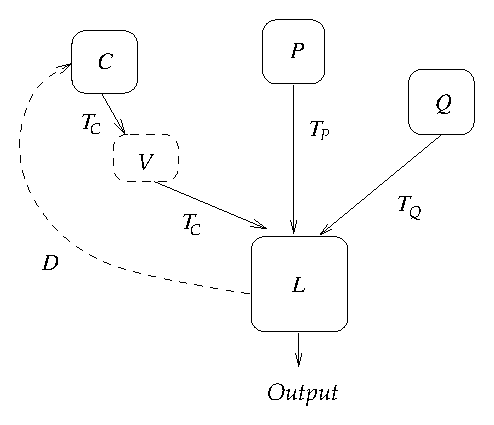
\includegraphics{Figures/tmstruct.eps}
& 
\hspace{-10mm}
$
\begin{array}[b]{rcl}
P &:& \text{Policy}\\
C &:& \text{Certificates}\\
Q &:& \text{Authorization Query}\\
V &:& \text{Certificate Validation}\\
L &:& \text{Authorization Mechanism}\\
T_P &:& \text{Policy Compilation}\\
T_C &:& \text{Credential Encoding}\\
T_Q &:& \text{Query Compilation}\\
D &:& \text{Distributed Certificate Discovery}\\
\end{array}
$
\end{tabular}
\vspace{2mm}
\end{fpfig}
}

% Figures Related to SpartanRPC and Sprocket
%%%%%%%%%%%%%%%%%%%%%%%%%%%%%%%%%%%%%%%%%%%%

\newcommand{\snowcloudfig}
{
\begin{fpfig}[t]
{A Snowcloud Sensor Node (L,C) and Harvester Device (R).}
{figure-snowcloud}
\vspace{3mm}
\begin{center}
\begin{tabular}{ccc}
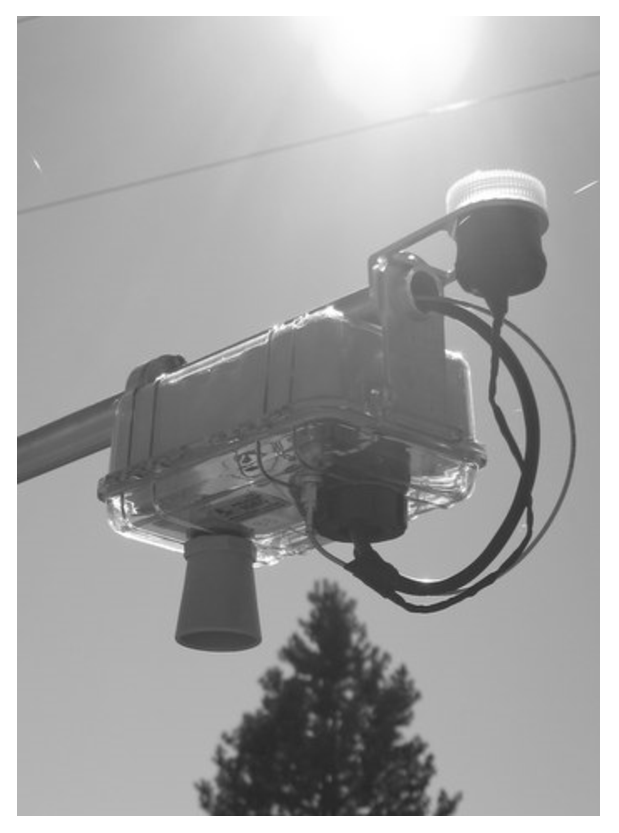
\includegraphics[scale=.35]{Figures/brainbox.eps}
& 
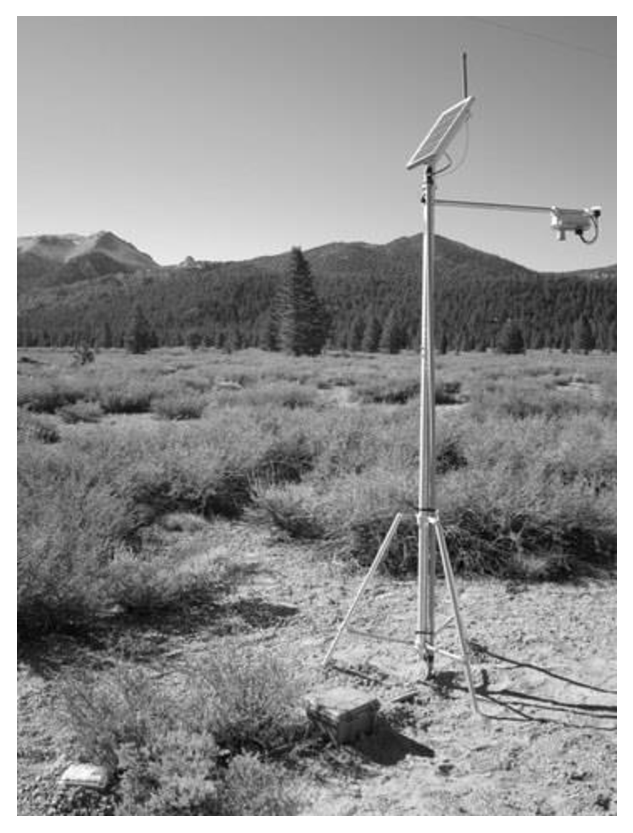
\includegraphics[scale=.35]{Figures/tower.eps} 
&
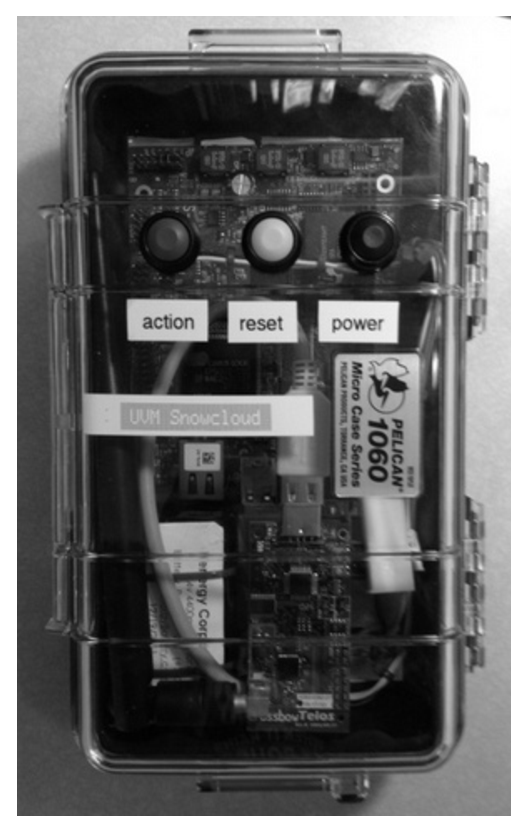
\includegraphics[scale=.35]{Figures/harvester.eps} 
\end{tabular}
\end{center}
\end{fpfig}
}

% Figures Related to nesT and Scalaness
%%%%%%%%%%%%%%%%%%%%%%%%%%%%%%%%%%%%%%%

\newcommand{\syntaxfig}
{
\begin{fpfig*}[!p]{Program Syntax of nesT}{figure-syntax}
\figsize
$$
\begin{array}{lc@{\ }l@{\hspace{-5mm}}r}
\s, \t & \defassign &
   \TVAR\ \mid \top \mid \intone\ \mid \inttwo \mid \intt \mid \undefv \mid & \textit{types} \\
       &            &
   \lc\tbindvec{\fdname}{\t}\rc \mid \t \idx{} \mid \t \kwstar \\

e      & \defassign &
    v \mid \lvalue \mid e \op e \mid \castto{\t}{e} \mid \fname\blok{} \mid \lvalue = e \mid \mid \& \lvalue \mid e \rhd e \mid & \textit{expressions} \\
       &            &
    \kwif\ (e)\  e\ \kwelse\ e \mid \kwwhile\ (e)\  e \mid e; e \mid \kwpost\ \fname\blok{\,} &\\

\lvalue & \defassign &
    x \mid e\idx{e} \mid e.\fdname \mid \kwstar e & \textit{l-values} \\

v       & \defassign &
    \neight \mid \nsixtn \mid \undefv & \textit{base values} \\
% \mv &\defassign& v \mid  
%  \arr{\vect \bn} \mid \lc \vect{\fdname = \bn} \rc & 
%\textit{values in memory}\\ 

\mathit{op} & \defassign &
    + \mid \kwstar \mid \texttt{\&\&} \mid \texttt{==} \mid \,\ldots & \textit{operations} \\

\id         & \defassign &
    \fname \mid x & \textit{identifiers} \\

c           & \defassign & \fname(\vpdecl\,) : \t = \{ e \}& \textit{command definition}\\

s           & \defassign & \fname(\vpdecl\,) : \t & \textit{command signature}\\

d           & \defassign &
    \xlet{\t}{x}{e} \mid \xlet{\t}{x}{\arr{\vect{e}}} \mid \xlet{\t}{x}{\lc \defvec{\fdname}{e} \rc} \mid c & \textit{declarations} \\

\tpdecl     & \defassign & \subtvec{\TVAR}{\t} & \textit{type parameters} \\

\vpdecl     & \defassign & \tbindvec{\VAR}{\t} & \textit{value parameters} \\

\imports    & \defassign & \vect{s} & \textit{imports} \\

\exports    & \defassign & \vect{c} & \textit{exports} \\

\exportsty  & \defassign & \vect{s} & \textit{export signatures} \\

\mu         & \defassign &
    \margs{\tpdecl; \vpdecl}\lc  \imports; \decls \exports \rc  & \textit{module definitions}\\

\jmodtcat   & \defassign &
    \margs{\tpdecl; \vpdecl}\lc \imports; \exportsty \rc & \textit{module signatures}

\end{array} 
$$
\end{fpfig*}
}


\newcommand{\semanticssyntaxfig}
{ 
\begin{fpfig*}[t]{Syntactic Definitions for Dynamic Configurations}{figure-semanticssyntax}
\figsize
$$
\begin{array}{rcl@{\!\!}r}
\pi        & \defassign & \bn \mid \circ & \textit{l/r tags} \\
\kappa     & \defassign & \cval{\pi}{\mv} & \textit{dynamic objects}\\ 
\lvalue    & \defassign & \cdots \mid \cval{\bn}{\mv} \\
e          & \defassign & \cdots \mid \kappa \\
\mv        & \defassign & v \mid \bn \mid \arr{\vect{\kappa}} \mid \lc \defvec{\fdname}{\kappa} \rc &  \textit{dynamic values}\\ 
\flash     & \defassign & \tdefvec{\fname}{\t}{\blok{e}} & \textit{codebase} \\
\blockmem  & \defassign & \tdefvec{\blockno}{\t}{\mv} & \textit{memory} \\
%\rv & \defassign & \lb \mem,v\rb & \textit{runtime values} \\ 
%e & \defassign & \cdots \mid \rv & \textit{runtime expressions} \\ 
\envletter & \defassign & \context{}{} \mid \envletter; e \mid \kappa \idx{E} \mid E\idx{e} \mid E.\fdname  \mid   \kappa = \envletter \mid \envletter = e \mid a \castto{\t}{\envletter} \mid & \textit{evaluation\ contexts}\\
           &            & \kwstar \envletter \mid \&\envletter \mid \envletter \ \emph{op} \ e\ \mid \kappa\ \emph{op}\ \envletter \mid \kwif\ (\envletter)\ e\ \kwelse\ e\ \mid \kwwhile\ (E)\  e  \\ 
%{D} & \defassign & 
%    \xlet{\t}{x}{E} \mid 
%    \xlet{\t}{x}{\arr{\vect{\kappa}; E; \vect{e}}} \mid  & \textit{decl evaluation contexts}\%\  
% && \xlet{\t}{x}{\lc \defvec{f}{\kappa}; f = E; \defvec{f}{e}} \rc  \\ 
\ell       & \defassign & \bootseq{\vect{d}} \mid \runseq{e} & \textit{run levels} \\
%\\
%& & 
% \tlet{t}{\t}{E}; \vect{\decl} \mid \xlet{\t}{x}{E}; \vect{\decl}
%\\
%\lenvletter & \defassign & m\idx{E} \mid E.\fdname 
% \mid \kwstar E & \textit{evaluation lcontexts}
\end{array}
$$
\end{fpfig*}
}


\newcommand{\coresemanticsfig}
{\begin{fpfig*}[t]{Dynamic Semantics of Selected Expressions}{figure-coresemantics}
\figsize
\begin{mathpar}
\inferrule[ArrIdx]
{}
{ \blockmem, \cval{\bn}{\arr{\vect{\kappa}}}\idx{\cval{\pi}{n}} \compute \blockmem, \kappa_n}

%\inferrule[Select]
%{}
%{ \blockmem, \cval{\bn}{\lc \vect{\fdname} = \vect{\kappa} \rc}.\fdname_n \compute \blockmem,% 
% \kappa_n}
%
\inferrule[Star]
{}
{\blockmem, \kwstar\cval{\pi}{\bn} \compute \blockmem, \cval{\bn}{\blockmem(\bn)}}

\inferrule[AddrOf]
{}
{\blockmem, \&\cval{\bn}{\mv} \compute \blockmem, \cval{\circ}{\bn}}

\inferrule[Cast]
{}
{ 
\blockmem, \castto{\t}{\kappa} \compute 
   \docast{\t}{\kappa}{\blockmem}
}

\inferrule[Assign]
{}
{\blockmem, \cval{\bn}{\mv_1} = \cval{\pi}{\mv_2} \compute \blockmem[\bn \mapsto \mv_2], 
 \cval{\pi}{\mv_2}}

%\inferrule[BinaryOp]
%{\fundef{opsem}(\mathit{op}, \mv_1, \mv_2) = \mv}
%{\blockmem, \cval{\pi_1}{\mv_1}\ \mathit{op}\ \cval{\pi_2}{\mv_2} \compute 
%  \blockmem, \cval{\circ}{\mv}}
%
\inferrule[Call]
{\flash(\fname) = \blok{e}}
{\blockmem, \fname() \compute \blockmem, e}

%\inferrule[Alloc]
%{}
%{\blockmem, \kwmalloc (\tau) \compute \funalloc(\tau,\blockmem)}
%
%\inferrule[Type]
%{}
%{\blockmem, \tau \compute \blockmem \uplus \lc \bn : \typet{\tau} = \tau\rc, \bn}
%
\inferrule[Int]
{}
{\blockmem, n \compute \blockmem, \cval{\circ}{n}}

%\inferrule[Null]
%{}
%{\blockmem, \undefv \compute \blockmem, \cval{\circ}{\undefv}}
%
%\inferrule[IfTrue]
%{n \ne 0}
%{\blockmem, \kwif\ (\cval{\pi}{n})\  e_1\ \kwelse\ e_2  \compute \blockmem, e_1 }
%
%\inferrule[IfFalse]
%{}
%{\blockmem, \kwif\ (\cval{\pi}{0})\  e_1\ \kwelse\ e_2  \compute \blockmem, e_2 }
%
%\inferrule[Sequence]
%{}
%{ \blockmem, \bn; e  \compute  \blockmem, e }
%
\inferrule[While]
{}
{ \blockmem, \kwwhile\ (e_1)\  e_2 \compute  \blockmem, \kwif(e_1)\ e_2; \kwwhile\ (e_1)\  e_2\ \kwelse\ \undefv}

\inferrule[Context]
{\blockmem,    e \compute  \blockmem, e'}
{\blockmem,    \context{E}{e} \compute  \blockmem,  \context{E}{e'}
}
\end{mathpar}
\end{fpfig*}
}

\newcommand{\lvaluesemanticsfig}
{
\begin{figure}[t]
\figurebox{

\begin{mathpar}
\inferrule[AssignCong]
{\blockmem, \lvalue \lcompute \blockmem', \lvalue'}
{\blockmem, \lvalue = e \compute \blockmem', \lvalue' = e}

\inferrule[ArrIdx]
{
\blockmem(\bn') = n \\ \blockmem(\bn)(n) = \bn_n
}
{ \blockmem, \bn\idx{\bn'} \lcompute \blockmem, \bn_n}

\inferrule[Select]
{\blockmem(\bn)(\fdname) = \bn_\fdname}
{\blockmem, \bn.\fdname \lcompute \blockmem, \bn_\fdname}

\inferrule[Star]
{}
{\blockmem, \kwstar\bn \lcompute \blockmem, \blockmem(\bn)}

\inferrule[ELContext]
{\blockmem,    e \compute  \blockmem, e'}
{\blockmem,    \lenv{}{e} \lcompute  \blockmem,  \lenv{}{e'}}

\inferrule[LEContextV]
{\blockmem,    \lenv{}{\bn'} \lcompute  \blockmem, \bn}
{\blockmem,    \env{}{\lenv{}{\bn'}} \compute  \blockmem,
  \env{}{\blockmem(\bn)}}

\inferrule[LEContextE]
{\blockmem,    \lenv{}{e} \lcompute  \blockmem, \lenv{}{e'} }
{\blockmem,    \env{}{\lenv{}{e}} \compute  \blockmem,  \env{}{\lenv{}{e'}}}
\end{mathpar}
}
\caption{Dynamic Semantics of lvalues} 
\label{fig:nest-lvaluesemantics}
\label{figure-lvaluesemantics}
\end{figure}
}

\newcommand{\modsemanticsfig}
{
\begin{fpfig*}[t]{Dynamic Semantics of Module Construction}{figure-modsemantics}
\figsize
\begin{mathpar}
\inferrule[Mod]
{ v = \margs{\tpdecl, \vpdecl}\lc \imports; \vect{\decl}; \exports \rc}
{\blockmem, v \compute \blockmem \uplus \lc \bn : \modty(v) = v \rc, \bn}


\inferrule[ModInst]
{
\blockmem(m) = \margs{\vect{t \subtype \t'}; \vect{x : \tau''}
   }\lc  \imports; \vect{\decl}; \exports \rc\\
\serialize(\vect{x}, \t''[\vect{\t}/\vect{t}], \vect{\bn}) = \vect{\decl'}
}
{\blockmem,  \bn \margs{\vect{\t},\vect{\bn}}  \compute 
  \blockmem, \margs{}\lc\imports; \vect{\decl} @ \vect{\decl'}; \exports \rc[\vect{\t}/\vect{t}]
}

\inferrule[ModWire]
{
\blockmem(\bn_1) = \margs{}\lc  \imports_1; \vect{\decl_1}; \exports_1 \rc\\
\blockmem(\bn_2) = \margs{}\lc  \imports_2; \vect{\decl_2}; \exports_2 \rc\\\\
\vect{\decl_3} = \exports_2 \restr \dom(\imports_1) \\
\imports' = (\imports_1 \maploosemerge \imports_2) / \exports_2
}
{\blockmem, \bn_1 \modwire \bn_2 \compute \blockmem, 
  \margs{}
  \lc \imports' ; \vect{\decl_2} @ \vect{\decl_3} @ \vect{\decl_1}; \exports_1 \rc} 

\inferrule[Validate]
{\blockmem(\bn) = \margs{}\lc\ ; \vect{\decl}; \exports\rc }
{\blockmem, \kwrun\ \bn \compute \blockmem, \undefv}
\end{mathpar}
\end{fpfig*}
}

\newcommand{\subjudgefig}
{
\begin{fpfig*}[t]{Subtyping Rules}{figure-subjudge}
\figsize
\begin{mathpar}
\inferrule[ReflS]
{}
{\subjudge{\tpdecl}{\tau}{\tau}}

\inferrule[TopS]
{}
{\subjudge{\tpdecl}{\tau}{\top}}

\inferrule[TransS]
{\subjudge{\tpdecl}{\tpdecl(t)}{\tau}}
{\subjudge{\tpdecl}{t}{\tau}}

\inferrule[UintS]
{}
{\subjudge{\tpdecl}{\intone}{\inttwo \subtype \intt}}

\inferrule[FnBodyS]
{\subjudge{\tpdecl}{\t_1}{\t_2}}
{\subjudge{\tpdecl}{\blok{\t_1}}{\blok{\t_2}}}

\inferrule[StructS]
{\tpdecl \vdash \vect{\t_1 \subtype \t_3}}
{\subjudge{\tpdecl}{\lc\vect{\fdname_1 : \t_1}
  \uplus \vect{\fdname_2 : \t_2} \rc}{\lc\vect{\fdname_1 : \t_3}\rc}}
%
%\inferrule[TypeS]
%{\subjudge{\tpdecl}{\tau}{\tau'}}
%{\subjudge{\tpdecl}{\typet{\tau}}{\typet{\tau'}}}
%
%\inferrule[ExistsS]
%{\subjudge{\tpdecl; t\subtype \tau}{\tau_0 }{\tau_1}}
%{\subjudge{\tpdecl}{(\texist{t \subtype \tau}{\tau_0})} 
%{(\texist{t \subtype\tau}{\tau_1})}}
%
%\inferrule[ModS]
%{
%\subjudge{\tpdecl[\tpdecl_0]}{\vpdecl_2}{\vpdecl_1} \\ 
%\subjudge{\tpdecl[\tpdecl_0]}{\imports_2}{\imports_1} \\ 
%\subjudge{\tpdecl[\tpdecl_0]}{\exportsty_1}{\exportsty_2}
%}
%{\subjudge{\tpdecl}
% {\margs{\tpdecl_0, \vpdecl_1 }\lc \imports_1, \exportsty_1 \uplus \exportsty \rc}
% {\margs{\tpdecl_0, \vpdecl_2 }\lc \imports_2 \uplus \imports, \exportsty_2 \rc}}
\end{mathpar}
\end{fpfig*}
}

\newcommand{\selectsubjudgefig}
{
\begin{fpfig*}[t]{Selected DnesT Subtyping Rules}{figure-selectsubjudge}
\figsize
\begin{mathpar}
\inferrule[UintS]
{}
{\subjudge{\tpdecl}{\intone}{\inttwo \subtype \intt}}

\inferrule[StructS]
{}
{\subjudge{\tpdecl}{\lc\vect{\fdname_1 : \t_1}
  \uplus \vect{\fdname_2 : \t_2} \rc}{\lc\vect{\fdname_1 : \t_1}\rc}}

\inferrule[ModS]
{
\subjudge{\tpdecl[\tpdecl_0]}{\vpdecl_2}{\vpdecl_1} \\ 
\subjudge{\tpdecl[\tpdecl_0]}{\imports_2}{\imports_1} \\ 
\subjudge{\tpdecl[\tpdecl_0]}{\exportsty_1}{\exportsty_2}
}
{\subjudge{\tpdecl}
 {\margs{\tpdecl_0, \vpdecl_1 }\lc \imports_1, \exportsty_1 \uplus \exportsty \rc}
 {\margs{\tpdecl_0, \vpdecl_2 }\lc \imports_2 \uplus \imports, \exportsty_2 \rc}}
\end{mathpar}
\end{fpfig*}
}

\newcommand{\coretypingfig}
{
\begin{fpfig*}[t]{Typing Rules for Selected DnesT Expressions}{figure-coretyping}
\figsize
\begin{mathpar}
%\inferrule[SequenceT]
%{\tenv,\tpdecl \vdash e_0 : \texist{\tpdecl_0}{\s_0} \\ 
%\tenv,\tpdecl \vdash e_1 : \texist{\tpdecl_1}{\s_1}}
%{\tenv,\tpdecl \vdash e_0 ; e_1 : \texist{\tpdecl_0 \maploosemerge \tpdecl_1}{\s_1}}
%
\inferrule[CastT]
{\tenv,\tpdecl \vdash e : \t \\ T \vdash \compatible{\t}{\s}}
{\tenv,\tpdecl \vdash (\s) e : \s}

\inferrule[CallT]
{\tenv,\tpdecl \vdash \fname : \s\\
\tpdecl  \vdash \s \promote \blok{\t}}
{\tenv,\tpdecl \vdash \fname() : \t}

%\inferrule[CondT]
%{\tenv, \tpdecl \vdash e_1 : \s_1 \\ 
% \tenv, \tpdecl \vdash e_2 : \s_2 \\
% \tenv, \tpdecl \vdash e_3 : \s_3 \\
% \tpdecl \vdash \s_1 \subtype \intt \\  
% \tpdecl \vdash \s_2 \promote \undefv \\  
% \tpdecl \vdash \s_3 \promote \undefv
% }
% {\tenv,\tpdecl \vdash \eite{e_1}{e_2}{e_3} : \undefv}
%
\inferrule[AssignT]
{\tenv, \tpdecl \vdash e_1 : \s_1 \\ 
 \tenv, \tpdecl \vdash e_2 : \s_2 \\
 \tpdecl \vdash \s_2 \subtype \s_1 
}
{\tenv,\tpdecl \vdash e_1 = e_2 : \s_1}

%\inferrule[AllocT]
%{}
%{\tenv,\tpdecl \vdash \kwmalloc(\t) : \t\kwstar}
%
\inferrule[StarT]
{
 \tenv,\tpdecl \vdash e : \s \\ 
 \tpdecl \vdash \s \promote \t\kwstar 
}
{\tenv,\tpdecl \vdash \kwstar e : \t}

\inferrule[NameT]
{\tenv(\identifier) = \t}
{\tenv,\tpdecl \vdash \identifier : \t}

\inferrule[IndexT]
{
 \tenv, \tpdecl \vdash e_1 : \s_1 \\ 
 \tenv, \tpdecl \vdash e_2 : \s_2 \\
 \tpdecl \vdash \s_1 \promote \t \idx{} \\
 \tpdecl \vdash \s_2 \subtype \intt 
}
{\tenv,\tpdecl \vdash e_1 \idx{e_2} : \t}

%\inferrule[ArrayIncrT]
%{
% \tenv, \tpdecl \vdash e_1 : \s_1 \\ 
% \tenv, \tpdecl \vdash e_2 : \s_2 \\
% \tpdecl \vdash \s_1 \promote \t \idx{} \\
% \tpdecl \vdash \s_2 \subtype \intt 
%}
%{\tenv,\tpdecl \vdash e_1 \pluseq e_2 : \t \idx{}}

%\inferrule[BlockT]
%{\tenv,\tpdecl \vdash e : \texist{\tpdecl'}{\s}}
%{\tenv,\tpdecl \vdash \blok{e} : \texist{\tpdecl'}{\blok{\s}}}
%
\end{mathpar}
\end{fpfig*}
}

\newcommand{\declmodtypingfig}{
\begin{fpfig*}[t]{Selected Declaration and Module Typing Rules}{figure-declmodtyping}
\begin{mathpar}
% \xlet{\t}{x}{e} \mid \xlet{\t}{x}{\arr{\vect{e}}} \mid \xlet{\t}{x}{\lc \defvec{\fdname}{e} \rc} \mid \fname : \t =  \blok{e}
\inferrule[DeclsNoneT]
{ }
{\tenv, \tpdecl \vdash \varnothing : \varnothing}

\inferrule[DeclsSomeT]
{\tenv, \tpdecl \vdash d \Rightarrow (x : \t) \\ (x : \t) \tenv, \tpdecl \vdash \vect{d} : \tenv'}
{\tenv, \tpdecl \vdash d \vect{d} : (x : \t) \tenv'}

\inferrule[DeclBaseT]
{\tenv, \tpdecl \vdash e : \t}
{\tenv, \tpdecl \vdash \xlet{\t}{x}{e} \Rightarrow x : \t}

%\inferrule[DeclArrayT]
%{\tenv, \tpdecl \vdash \vect{e} : \t}
%{\tenv, \tpdecl \vdash \xlet{\t\idx{}}{x}{\arr{\vect{e}}} \Rightarrow x : \t \idx{}}
%
%\inferrule[DeclStructT]
%{\tenv, \tpdecl \vdash \vect{e} : \vect{\t}}
%{\tenv, \tpdecl \vdash \xlet{\t}{x}{\lc \defvec{\fdname}{e} \rc} \Rightarrow 
%  x : \lc \tbindvec{\fdname}{\t} \rc}
%
\inferrule[DeclFunT]
{\tenv, \tpdecl \vdash e : \t}
{\tenv, \tpdecl \vdash \fname : \blok{\t} = \blok{e} \Rightarrow 
  \fname : \blok{\t}}

\inferrule[ModuleT]
{ 
\imports @ \vpdecl, \tpdecl \vdash \vect{d} : \tenv \\
\tenv @ \imports @ \vpdecl, \tpdecl \vdash \exports : \exportsty 
}
{\margs{\tpdecl, \vpdecl}\lc \imports; \vect{\decl}; \exports \rc : 
  \margs{\tpdecl, \vpdecl}\lc \imports; \exportsty \rc}
\end{mathpar}
\end{fpfig*}
}

\newcommand{\modtypingfig}{
\begin{fpfig*}[t]{Module Typing Rule}{figure-modtyping}
\begin{mathpar}
\inferrule[ModT]
{
\vpdecl\, @\, \imports, \tpdecl \vdash \vect{d} : \tenv\\
\vpdecl\, @\, \imports\, @\, \tenv, \tpdecl \vdash \exports : \exportsty
}
{
\margs{\tpdecl; \vpdecl} 
\lc  
  \imports;
  \vect{d};
  \exports
\rc
:  
\margs{\tpdecl; \vpdecl} 
\lc  
  \imports,
  \exportsty
\rc
}
\end{mathpar}
\end{fpfig*}
}

\newcommand{\modoptypingfig}{
\begin{fpfig*}[t]{Module Typing Rules}{figure-modtyping}
\figsize
\begin{mathpar}
\inferrule[ModT]
{
\vpdecl_0[\imports], 
\tpdecl_1[\tpdecl_0] \vdash \exports
}
{
\tenv_1, \tpdecl_1 \vdash \margs{\tpdecl_0; \vpdecl_0} 
\lc  
  \imports,
  \exports
\rc
:  
\modty{(\margs{\tpdecl_0; \vpdecl_0} 
\lc  
  \imports,
  \exports
\rc)}
}

\inferrule[ModInstT]
{
\tenv, \tpdecl \vdash e : \texist{\tpdecl'}{\s}\\
\tenv,\tpdecl \vdash \tbindvec{e}{\texist{\tpdecl}{\s}}\\
\tpdecl'' = (\maploosemerge\vect\tpdecl) \maploosemerge \tpdecl'\\
\tpdecl \maploosemerge \tpdecl'' \vdash \s \promote
   \margs{\subtvec{t}{\t_0};\tbindvec{\fname}{\t_1}} \lc 
  \imports; \exportsty \rc \\
\tpdecl \maploosemerge \tpdecl'' \vdash \subtvec{\t}{\t_0}\\
 \vect{\texist{\tpdecl}{\s}} = \vect{\t_1}[\vect{\tau/t}] 
}
{
\tenv,\tpdecl \vdash 
e \margs{\vect{\t},\vect{e}} 
: 
\texist{\tpdecl''}{(\margs{}\lc \imports;  \exportsty \rc)
[\subnvec{\t}{t}]}
}

\inferrule[ModCompT]
{
\tenv,\tpdecl \vdash e_0 : \texist{\tpdecl_0}{\s_o}\\
\tenv,\tpdecl \vdash e_1 : \texist{\tpdecl_1}{\s_1}\\
\tpdecl' = \tpdecl_0 \maploosemerge \tpdecl_1\\
\tpdecl \maploosemerge \tpdecl' \vdash \s_0 \promote  \margs{\tpdecl_0',\vpdecl_0} \lc 
  \imports_0;   \exportsty_0 \rc \\
\tpdecl \maploosemerge \tpdecl' \vdash \s_1 \promote \margs{\tpdecl_1',\vpdecl_1} \lc 
  \imports_1;   \exportsty_1\rc }
{
\tenv,\tpdecl \vdash e_0 \modcomp e_1 : 
\texist{\tpdecl'}{\margs{\tpdecl_0' \maploosemerge \tpdecl_1', \vpdecl_0 \maploosemerge \vpdecl_1} \lc 
(\imports_0 \maploosemerge \imports_1) / \dom(\exportsty); \exportsty_0 \uplus \exportsty_1 \rc}
}

\inferrule[ValidateT]
{
\tenv, \tpdecl \vdash e : \texist{\tpdecl'}{\s} \\ 
 \tpdecl \maploosemerge \tpdecl' \vdash \s \promote  \margs{}\lc ;   \exportsty \rc \\ 
}
{\tenv,\tpdecl \vdash \kwrun\  e: \texist{\tpdecl'}{\undefv}}

\inferrule[TypedefT]
{
\tenv, \tpdecl \vdash e_0 : \texist{\tpdecl_0}{\s_0}\\
\tenv, \tpdecl[t \subtype \t] \vdash e_1 : \texist{\tpdecl_1}{\s_1}\\
\tpdecl' = \tpdecl_0 \maploosemerge \tpdecl_1 \maploosemerge [t \subtype \t] \\
\tpdecl \maploosemerge \tpdecl' \vdash \s_0 \subtype \typet{\t} 
}
{
\tenv, \tpdecl \vdash \tlet{t}{\t}{e_0}{e_1} : \texist{\tpdecl'}{\s_1}
}
\end{mathpar}
\end{fpfig*}
}

\newcommand{\configtypingfig}
{
\begin{fpfig*}[t]{Memory, Codebase, and Configuration Typing}{figure-configtyping}
\figsize
\begin{mathpar}
\inferrule[ValDef]
{v \text{ not a memory location} \\ 
 \tenv[\vect{\localname : \t}], \tpdecl \vdash v : \t' \\ 
 \subjudge{\tpdecl}{\t'}{\t}
}
{\tenv, \tpdecl, \vect{\localname : \t = \mv} \vdash v : \t}

\inferrule[ArrayM]
{\forall 0 \le i < n . \ascript(\mv(i), \exports) = \t}
{\tenv, \tpdecl, \exports \vdash \mv : \t\idx{n}}

\inferrule[StructM]
{
 \vect{\ascript(\bn, \exports)} = \vect{\t}
}
{\tenv, \tpdecl, \exports \vdash \lc 
 \vect{\fdname = \bn} \rc : \lc\vect{\fdname : \t} \rc}

\inferrule[PtrM]
{\ascript(\bn, \exports) = \t}
{\tenv, \tpdecl, \exports \vdash \bn : \t\kwstar }

\inferrule[UninitM]
{\exports(\bn) = \undefv}
{\tenv, \tpdecl, \exports \vdash \bn : \t\kwstar }

\inferrule[DefsT]
{\forall (\localname : \t = \mv) \in \exports . \tenv, \tpdecl, 
 \exports \vdash \mv : \t}
{\tenv, \tpdecl \vdash \exports}

\inferrule[Config]
{ \forall \fname() \in \tasks . \fname \in \dom(\flash) \\ 
  \varnothing, \varnothing \vdash \flash[\blockmem] \\ \varnothing, \varnothing, \flash[\blockmem] \vdash e : \texist{\tpdecl}{\s}
}
{(\flash,\tasks,\blockmem,e) : (\tpdecl, \s)}
\end{mathpar}
\end{fpfig*}
}

\newcommand{\tasksemanticsfig}
{
\begin{fpfig*}[t]{Semantics of Tasks and Configurations}{figure-tasksemantics}
\begin{mathpar}
\figsize
\inferrule[CoreStep]
{\blockmem, e  \compute \blockmem',  e'}
{\tasks, \blockmem, e  \tcompute{} \tasks, \blockmem',  e'}

\inferrule[Post]
{}
{\tasks, \blockmem,  \context{E}{\kwpost\ \fname\blok{}}  \tcompute{}
 \addt(\tasks,\fname\blok{}), \blockmem,  \context{E}{\undefv}}

\inferrule[TaskStart]
{\nextt(\tasks) = \tasks',\fname\blok{}}
{\tasks, \blockmem, \bn  \tcompute{}
  \tasks', \blockmem,  \fname\blok{}}
\end{mathpar}
\end{fpfig*}
}

\newcommand{\declsemanticsfig}
{
\begin{fpfig*}[t]{Semantics of Declarations}{figure-declsemantics}
\begin{mathpar}
\inferrule[DeclContext]
{\flash \vdash \tasks, \bm, e \compute \tasks', \bm', e'}
{\flash, \tasks, \bm, D[e] \vect{\decl} \compute \flash, \tasks', \bm', D[e'] \vect{\decl}}

\inferrule[BaseInit]
{\kappa = \cval{\bn}{\mv} \\ \bn \not\in \dom(\bm)}
{\flash, \tasks, \bm,(\xlet{\t}{x}{\cval{\pi}{\mv}}) \vect{\decl} \compute 
 \flash, \tasks, (\bn : \t = \mv)\bm, \vect{\decl}[\kappa/x]}

\inferrule[StructInit]
{\kappa = \cval{\bn}{\mv} \\ \bn \not\in \dom(\bm)}
{\flash, \tasks, \bm,(\xlet{\t}{x}{\mv}) \vect{\decl} \compute 
 \flash, \tasks, (\bn : \t = \mv)\bm, \vect{\decl}[\kappa/x]}

\inferrule[FDecl]
{}
{\flash, \tasks, \bm, (\fname : \t = \blok{e}) \vect{\decl} \compute 
 (\fname : \t = \blok{e}) \flash, \tasks, \bm, \vect{\decl}}
\end{mathpar}
\end{fpfig*}
}

\newcommand{\bootloadsemanticsfig}
{
\begin{fpfig*}[t]{Boot and Runtime Semantics}{figure-bootloadsemantics}
\begin{mathpar}
\inferrule[RunTime]
{\flash \vdash \tasks,\bm,e \compute \tasks',\bm',e'}
{\flash,\tasks,\bm,\runseq{e} \compute \flash,\tasks',\bm',\runseq{e'}}

\inferrule[BootTime]
{\flash,\tasks,\bm,\vect{d} \compute \flash',\tasks',\bm',\vect{d}'}
{\flash,\tasks,\bm,\bootseq{\vect{d}} \compute 
 \flash',\tasks',\bm',\bootseq{\vect{d}'}}

\inferrule[RunStart]
{}
{\flash,\tasks,\bm,\bootseq{\emptyset} \compute 
 \flash,\tasks,\bm,\runseq{\textrm{main}\blok{}}}
\end{mathpar}
\end{fpfig*}
}

\newcommand{\scalanesssyntaxfig}
{
\begin{fpfig*}[t]{The Syntax of DScalaness}{figure-scalanesssyntax}
$$
\begin{array}{rcl@{\hspace{3mm}}r}
\\[-4mm]%
\tt{L} & ::= & \gclass{C}{\gbounds{X}{N}}{N}{\fieldvec{T}{f};\ K\ \ttvec{M}} & \gdesc{class definitions}\\[1mm]
\tt{K} & ::= & \init{C}{\tdecls{T}{f}}{\super(\ttvec{f});\ \this.\ttvec{f}=\ttvec{f};} & \gdesc{constructors}\\[1mm]
\tt{M} & ::= & \meth{T}{m}{\tdecls{T}{x}}{\return{e};} & \gdesc{methods}\\[1mm]
\tt{e} & ::= & \tt{x} \mid \select{e}{f} \mid \send{e}{m}{\ttvec{e}} \mid \gnew{C}{\ttvec{T}}{\ttvec{e}}  \mid \cast{N}{e} \mid \mutate{\select{e}{f}}{e} \mid \tt{l} \mid  & \gdesc{expressions}\\
       &     & \jdef{x}{T}{e}{e} \mid % \jtlet{x}{\tt{T}}{e}{e} \mid \\ & & 
\jmodval \mid \jwire{\tt{e}}{\tt{e}} \mid \jinst{e}{\ttvec{e};\ttvec{e}} \mid \jimage{\tt{e}} \mid \\
       &     & \abbrvt{X(\ttvec{X})}{T}{e} \\[1mm]
\tt{T} & ::= & \tt{X} \mid \tt{N} \mid \jmodt{\tpdecl}{\jmodtcat} & \gdesc{scala level types} \\[1mm]
\tt{N} & ::= & \jinst{C}{\ttvec{T}} & \gdesc{class types}\\[1mm]
\tt{l} & ::= & \jref{\tt{p}}{N} & \gdesc{references}
\end{array}
$$
\end{fpfig*}
}

\newcommand{\jmodsemanticsfig}
{
\begin{fpfig*}[t]{DScalaness Module Semantics}{figure-jmodsemantics}
\begin{mathpar}
\inferrule[ModInst]
{
\jmodval = \margs{\subtvec{t}{\t}; \tbindvec{x}{\s}}
   \lc  \imports; \vect{\decl}; \exports \rc\\
\serialize(\vect{x}, \vect{\s}, \ttvec{l}) = \vect{\decl'}
}
{ 
 \jinst{\jmodval}{\jref{\vect{p}}{\jinst{MetaType}{\ttvec{T}}};\,\ttvec{l}}  \rightarrow 
   \margs{}\lc\imports; \vect{\decl'} @ \vect{\decl}; \exports \rc[\codt{\ttvec{T}}/\vect{t}]
}

\inferrule[ModWire]
{\imports = (\imports_1 / \dom(\exports_2)) @ \imports_2 \\
 \vect{d} = \vect{d}_2 @ \restrict{\exports_2}{\dom(\imports_1)} 
}
{\jwire{\margs{\tpdecl_1,\vpdecl_1} \lc  \imports_1; \vect{d}_1; \exports_1 \rc}
       {\margs{\tpdecl_2,\vpdecl_2} \lc  \imports_2; \vect{d}_2; \exports_2 \rc}\\\\
 \rightarrow\\\\
   \margs{\tpdecl_1 \maploosemerge \tpdecl_2,\vpdecl_1 \maploosemerge \vpdecl_2} 
    \lc  \imports; \vect{\decl} \maploosemerge \vect{\decl}_1; \exports_1 \rc
}

\inferrule[ModImage]
{}
{\jimage{(\margs{}\lc ; \vect{d}; \exports \rc)} \rightarrow \margs{}\lc ; \vect{d}; \exports \rc}
\end{mathpar}
\end{fpfig*}
}

\newcommand{\scalanesstypingfig}
{
\begin{fpfig*}[t]{DScalaness Module Typing Rules}{figure-scalanesstyping}
\begin{mathpar}
\inferrule[ModT]
{\jmodval : \jmodtcat \text{\ in\ nesT\ type\ checking}}
{\Gamma \vdash \jmodval : \jmodt{\varnothing}{\jmodtcat}}

\inferrule[ModInstT]
{\Gamma \vdash \tt{e} : \jmodt{\varnothing}{\margs{\vect{t} \subtype \vect{\t}_1; 
 \vect{x} \subtype \vect{\t}_2} \lc 
  \imports; \exportsty \rc}\\
 \Gamma \vdash \ttvec{s} : \jinst{MetaType}{\ttvec{T}_1}\\
 \Gamma \vdash \ttvec{e}_2 : \ttvec{T}_2 \\
 \vdash \codt{\ttvec{T}_1} \subtype \vect{\t}_1\\
 \vdash \codt{\ttvec{T}_2} \subtype \vect{\t}_2
}
{\Gamma \vdash \jinst{e}{\ttvec{s}; \ttvec{e}_2} : \jmodt{\vect{s}\subtype \codt{\ttvec{T}_1}}{\margs{} \lc 
  \imports[\vect{s}/\vect{t}]; \exportsty[\vect{s}/\vect{t}] \rc} }

\inferrule[ModWireT]
{
 \Gamma \vdash \tt{e}_1 : \jmodt{\tpdecl_1}{\margs{}\lc\imports_1; \exportsty_1 \rc}\\
 \Gamma \vdash \tt{e}_2 : \jmodt{\tpdecl_2}{\margs{}\lc\imports_2; \exportsty_2 \rc} \\
 \imports = (\imports_1 / \dom(\exportsty_2)) @ \imports_2 \\
}
{\Gamma \vdash \jwire{\tt{e}_1}{\tt{e}_2} : 
 \jmodt{\tpdecl_1 \maploosemerge \tpdecl_2}{\margs{}\lc\imports; \exportsty_1 \rc}}

\inferrule[ModImageT]
{
  \Gamma \vdash \tt{e} : \jmodt{\tpdecl}{\margs{}\lc \imports; \exportsty \rc} \\
  \text{main}() : \t \in \exportsty
}
{
  \Gamma \vdash \jimage{\tt{e}} : \jmodt{\tpdecl}{\margs{}\lc \imports; \exportsty \rc}
}
\end{mathpar}
\end{fpfig*}
}


% I like \oneandhalfspace better. Too bad \doublespace is now required.
\newcommand{\primaryspacing}{\doublespace}
\primaryspacing

% Now begins my thesis/dissertation defense information
\defensedate{October 25, 2013}
\dissertation                      %% or \thesis
\doctorphilosophy                  %% or \doctorphilosophy or \masterarts
\cs                                %% This is the only speciality defined.
\gradyear{2014}                    %% The year in which the degree will be conferred
\jangrad                           %% \maygrad or \octgrad, \jangrad, \margrad, or \maygrad
\advisor{Christian Skalka, Ph.D.}  %% e.g. \advisor{Xindong Wu, Ph.D.}
\readerone{Alan Ling, Ph.D.}
\readertwo{Margaret Eppstein, Ph.D.}
\chair{Jeffrey Frolik, Ph.D.}

%%%%%%%%%%
% Document
%%%%%%%%%%

\begin{document}

\title{Trust Management in Wireless Sensor Networks\\Using Direct and Staged Approaches}
\author{Peter C. Chapin}
\maketitle

% Committee Acceptance Form is page two
\stepcounter{page}
\makeacceptance
\pagenumbering{roman}


% The abstract is just text enclosed in the 'abstract' environment. It should be single spaced
% and has a one page limit.

\singlespace
\begin{abstract}
  Many embedded systems, such as wireless sensor networks, make use of highly resource
  constrained devices. Security in such systems, when it is used at all, tends to focus on
  keeping data confidential from outsiders or ensuring data integrity during communication.
  However as embedded systems from different administrative domains increasingly come into
  contact, for example via short hop radio links, a need arises for one system to allow partial
  access to its resources from adjoining systems. In this dissertation I explore two approaches
  to providing distributed trust management facilities to wireless sensor networks, although the
  techniques used could be applied to a variety of other embedded systems. The first is a direct
  approach using a secure remote procedure call mechanism called \textit{SpartanRPC}. The second
  is a staged approach using a two stage programming system called \textit{Scalaness/nesT}. In
  addition to describing these two approaches I also present the results of evaluating them in
  both test environments and with a realistic application. Both approaches are feasible but the
  staged approach is far more flexible and, depending on application requirements, more
  efficient.
\end{abstract}
\primaryspacing

\clearpage


\addcontentsline{toc}{chapter}{Dedication}

% To use \dedication environment, the command has to be defined in uvm-dissertation.sty.

\doublespace
\dedication \emph{\textbf{To my wife Sharon for her unwavering support, continuous
    encouragement, and patient tolerance, and to my father for showing me the value of
    education.}}
\primarspacing

%% Use the following command if you want the title "Dedication" showing on the top of the page.
%\chapter*{Dedication} \dedication \emph{\textbf{To my... }}

\clearpage



% Required by UVM.

\doublespace
\addcontentsline{toc}{chapter}{Acknowledgments}
\chapter*{Acknowledgments}

This dissertation would not have been possible without the assistance and guidance of many
people. I would especially like to thank my adviser Christian Skalka for many years of valuable
feedback. I would also like to thank my collaborators Sean Wang, Scott Smith, and especially
Simone Willet and Michael Watson for their invaluable assistance in making the work I describe
here a reality. Finally I'd like to thank the faculty and staff of the University of Vermont
Computer Science department for creating an environment that allowed me to flourish.

\primaryspacing



% Single space the lists, as recommended
\singlespace

\tableofcontents
\clearpage

\addcontentsline{toc}{chapter}{\listtablename}
\listoftables
\clearpage

\addcontentsline{toc}{chapter}{\listfigurename}
\listoffigures
\clearpage

% A list of symbols can go here, if any. Handle it like the Acknowledgements.
%\include{notation}

% Switch back to the primary spacing.
\primaryspacing

% Body of dissertation begins here.
\pagenumbering{arabic}

\chapter{Introduction}
\label{chapter-introduction}

Embedded systems present difficult programming challenges
\cite{Mottola:2011:PWS:1922649.1922656}. For reasons of size, power consumption, disposability,
or some combination of these things, embedded devices are often highly resource constrained. For
example, a typical device might have only 48~KiB of program ROM, 8~KiB of RAM (or less), and use
a small, 16~bit microcontroller running at only 8~MHz \cite{tmotesky-datasheet}. Yet embedded
applications are increasing in complexity and often provide mission-critical or even
safety-critical services. Such systems need to be both efficient and correct.

My interest is in the use of distributed trust management in resource constrained embedded
systems. Here \newterm{trust management} refers to a general approach for authorizing access to
resources in an environment where the identity of requesting principals is not known to the
authorizer. A trust management system provides a way for the authorizer to define an access
policy in terms of arbitrary certified attributes that the requester must possess. Many trust
management systems have been described in the literature \cite{chapin-skalka-wang-acmcs08}, and
they vary in complexity, expressiveness, and mathematical foundations. However, all attempt to
provide a formalized, well structured approach to the problem of access control in widely
distributed and dynamic environments.

Trust management systems are typically designed for use by authorizers with resource rich
machines such as is commonly used for file and web servers. Yet there are embedded applications
that could also benefit from trust management. For example, ``smart cars'' that communicate with
each other about road conditions and for traffic coordination
\cite{Seepold:2009:ESP:1641563.1641568}, or body area networks that provide medical monitoring
and intervention features \cite{Shnayder:2005:SNM:1098918.1098979,Chen:2011:BAN:1968858.1968873}
may encounter many unknown principals during their operation. The security and safety of these
applications will depend on their ability to distinguish trustworthy principals from unreliable
or malicious ones.

For reasons of space and time efficiency many embedded systems are programmed in low level
languages such as C. Programming at that level is complicated and error prone. It is desirable,
therefor, to provide programmers with convenient abstractions to shield them from low level
complexities. I believe, in particular, that these abstractions should be in the programming
language itself, and my work is about providing enriched languages that can be used to address
the needs of modern embedded systems. This \newterm{language-based} approach off-loads some of
the work of producing correct programs to the language compiler and runtime system. Language
features can be formally analyzed and rigorously tested once and then applied to many
applications. This is in contrast to each application being an ad-hoc construction of customized
components with limited use beyond the application for which they were created.

The value of formal foundations can not be overstated. In critical systems were safety or
security is at stake, a rigorous understanding of the mechanisms being used is essential. For
example, trust management systems that provide a precisely defined policy language are
preferable to systems that use informally described methods for specifying access control.

In this dissertation I focus on a kind of embedded system called a \newterm{wireless sensor
  network} (WSN). Such systems consist of a network of small sensors or actuators that are
connected by way of short hop wireless links. Commonly such networks include one or more base
stations, or ``hubs,'' with wider connectivity that serve as an interface between the sensor
network and external systems. Wireless sensor networks are an area of intense study with many
envisioned applications ranging from environment, asset, and structural monitoring to emergency
response \cite{Culler:2004:GEI:1018015.1018072,1038146}. Yet despite my use of sensor networks
to demonstrate the systems I describe, the techniques can be used with a wide range of embedded
applications.

I describe two approaches to solving the problem of providing trust management-style distributed
authorization in resource constrained embedded systems. The first approach is based on a new
remote procedure call (RPC) discipline called \textit{SpartanRPC}
\cite{chapin-skalka-SpartanRPC,chapin-skalka-SpartanRPCTR}. In this method all authorization
computations are done directly on the embedded devices. However, the complexity of the system is
hidden from the programmer behind a simple extension to the widely used nesC programming
language \cite{Gay-nesC-2003}. My implementation of this \emph{direct} approach is a compiler
called \textit{Sprocket} that takes an extended dialect of the nesC language as input and
outputs an equivalent program in ordinary nesC. In addition Sprocket outputs the necessary
runtime support to process authorization requests and policy statements in the $RT_0$ trust
management language \cite{Li:DRBTMF,Li:RRBTMF}.

The second approach I present is based on \newterm{staged programming}
\cite{Taha-MetaML,Sheard-TemplateHaskell,Mainland-Flask-2008,FramedML}. In a staged environment,
a first stage program is used to compose and specialize a lower level, second stage program.
Specialized code can often be considerably optimized. However, flexibility is retained because
the first stage program can be re-executed at a later time to re-specialize the second stage
program as needed.

Unlike many staging systems I am interested in the application of staging where the stages use
different programming languages and execute on different machines, i.e., in different address
spaces. When applied to embedded systems, the second and final stage must be in an embedded
systems language running on the embedded hardware, whereas the first stage need not be as
restricted.

In this dissertation I also describe \newterm{Scalaness} \cite{chapin-GPCE-2013}, an extension
of Scala \cite{PiS2} with features that allow the programmer to compose and specialize
components written in a reduced dialect of nesC called \newterm{nesT}. An important novel
feature of Scalaness is that it extends Scala's type system so that a well-typed Scalaness
program will always generate a well-typed nesT program. Thus the type correctness of the program
that ultimately runs on the embedded device is guaranteed by the first stage Scalaness compiler.

I chose Scala as the basis for my first stage language largely for pragmatic reasons. I wanted
to build a practical system that could be used for real applications. Scala is a rich language
that runs on the Java Virtual Machine (JVM) and thus has access to the Java ecosystem. Also the
Scala compiler has a plugin architecture, and I had hoped to implement Scalaness as a compiler
plugin. Unfortunately, as described in \autoref{chapter-scalaness-nest} that proved difficult
and Scalaness was instead implemented as a direct modification to the Scala compiler itself.

\section{Related Work}

% From the Trust Management paper.
% Isn't that entire paper just related work???

% From the TISSEC paper.

Extending sensor network software platforms with support for secure interactions between domains
has been studied in previous research on SSL for sensor networks \cite{10.1109/WAINA.2009.47}.
However, this work was focused on extending the Internet to sensor networks (aka ``IP for
WSNs''), whereas SpartanRPC is a more general system for enhancing secure communications
\emph{within} a sensor network. Research on sensor network security has also addressed secure
routing \cite{senroute-ahnj03}, link layer security \cite{karlog-tinysec-2004}, cryptography
\cite{bertoni-2006}, key distribution \cite{camtepe-bulent-05}, and hardware issues
\cite{perrig-2004}. In contrast to these low-level systems, SpartanRPC provides language-level
abstractions for secure RPC services. Perhaps even more closely related is a system for
establishing fine-grained, ``node-level'' policies in sensor networks
\cite{Claycomb:2011:NNL:1889383.1889450}. However, this work is more focused on group-based key
negotiation and distribution, and while it does offer a policy language, it is rooted in
implementation details and not as a separable specification. Also, that work does not provide a
language API for integrating their system into secure applications as does SpartanRPC.

Previous related work also illustrates interest in and useful applications of RPC in embedded
networks. For example, the Marionette system uses network layer RPC for remote (PC-based)
analysis and debugging of sensor networks \cite{whitehouse-marionette-2006}. The Fleck operating
system provides a small pre-defined set of RPC services for sensor network applications, while
the trustedFleck system extends this with a form a secure RPC
\cite{hu-secfleck-2009,Hu:2010:TTW:1806895.1806900}. S-RPC provides an RPC facility for sensor
networks that allows remote services to be added to the system dynamically \cite{5766863}.
SpartanRPC differs from these systems in that it extends the nesC programming language (unlike
trustedFleck) to allow programmer definition of secure RPC services (unlike S-RPC) that can be
accessed by nodes within the network itself (unlike Marionette). Our system is similar to and
inspired by TinyRPC \cite{may-tinyrpc-2007}, except the latter does not provide security and has
a different semantics that are not as expressive as our approach.

Teeny\textsc{lime} allows application programs to access an abstract ``tuple space'' that is the
union of tuple spaces on the local node and the immediately neighboring nodes
\cite{Costa:2007:PWS:1516124.1516153}. This provides an alternative to RPC for uniformly
accessing remote and local data. However, interaction with the middleware is by way of a
dedicated API; there is no attempt to provide a true RPC mechanism. Also Teeny\textsc{lime} does
not address issues of access control.

Secure Middleware for Embedded Peer to Peer systems (SMEPP) is a general framework for creating
security sensitive applications from a distributed network of embedded peers
\cite{Brogi:2008:SME:1363370.1363548}. SMEPP Light \cite{Vairo:2008:SMW:1594978.1595054} is a
reduced version of SMEPP to address the resource constraints of wireless sensor networks. SMEPP
Light provides a publish/subscribe communication model using directed diffusion
\cite{intanagonwiwat-2003} to distribute ``events'' to all subscribers and symmetric key
cryptography to provide confidentiality and data integrity within a group of nodes. However,
SMEPP Light is not integrated into a programming language and does not provide a remote
procedure call mechanism. Furthermore SMEPP Light only supports a simple model of access control
based on group membership.

High level macro\-programming languages such as Kairos \cite{springerlink:10.1007/1150259312},
and Regiment \cite{Newton:2007:RMS:1236360.1236422} provide a way to program the entire network
as a single entity. These systems attempt to hide not only the inter-node communication from the
programmer, but also the entire node level programs. SpartanRPC operates at a much lower level
and also, unlike these macro\-programming systems, addresses access control issues in networks
containing multiple security domains.

Whole network programming of wireless sensor networks has also been investigated using mobile
agents in systems such as Agilla \cite{Fok:2009:AMA:1552297.1552299} and Wiseman
\cite{Gonzalez-Valenzuela:2010:PMW:1891545.1891566}. However, like the macro\-programming
systems mentioned previously neither of these systems address issues related to access control
in the presence of multiple security domains.

% From the GPCE paper

The work described here follows the foundational \fml\ work \cite{FramedML};
\autoref{section-framedml} discusses how it serves as the theoretical underpinning of Scalaness.

The potential of applying metaprogramming to sensor networks was explored in the functional
sensor language Flask \cite{Mainland-Flask-2008}. Flask allows functional reactive programming
(FRP)-based stream combinators to be pre-computed before network deployment, but it is possible
to generate ill-typed Flask object code since cross-stage static type checking is not performed.
Hume \cite{Hume} is a domain specific language for real-time embedded device programming. It
includes a metaprogramming layer but that layer is more like nesC's configuration files in that
there is a very restricted syntax for a few special metaprogramming operations including
component wiring, macros, and code templating.

MetaML \cite{Taha-MetaML,DBLP:conf/icess/Taha04} and MetaHaskell \cite{mainland12} are
foundations my work builds on. MetaHaskell does support heterogeneous language staging where the
lower stage language is defined by a plug-in and several instantiations have been defined
including one for a low-level C-like language. Like our approach they guarantee type safety of
all lower-stage code produced. They use a more traditional metaprogramming model, however, not
the process-separated model needed for embedded systems metaprogramming and do not address the
issues of metaprogramming module composition and type specialization.

Lightweight Modular Staging \cite{Rompf-LMS} describes a method of expressing staged
computations using a Scala host framework without any compiler modifications. The approach
allows cross-stage type safety but also does not support dynamic type construction.

Actor based sensor metaprogramming has been studied in \cite{cheong07}; this work shares my
focus on high level dynamic reprogrammability but is untyped. More broadly, meta programming is
known to be useful for increasing the efficiency of systems applications. One example is Tempo
\cite{289140}, a system that integrates partial evaluation and type specialization for
increasing efficiency of systems applications. Ur \cite{UrPLDI10} allows for type safe meta
programming for web applications.

The units of staged code composition in nesT programming are \emph{modules}. Countless different
module systems exist, but they are primarily designed to achieve separate compilation and sound
linking \cite{Cardelli-1997}. My different design goal leads to different design choices in nesT
modules. For example, data crossing nesT module boundaries needs to conform to the property of
process separation, a non-issue in standard module system designs. In addition, nesT modules
allow values/types across the boundary of modules to be flexibly constructed, including dynamic
construction of types. Module systems such as ML modules \cite{macqueen84} and Units
\cite{flatt98units} allow types to be imported/exported as I also support. However, there are
several features of ML modules including type hiding that my system does not aim to support.

NesT modules are more expressive in their support of first class modules as values and the
possibility of dynamic construction of ``type exports.'' That said, first class modules are not
new \cite{99620,ancona01calculus}, The novelty of nesT arises in its application to program
staging and the incorporation of dynamic type construction.

The type parametricity of System F and F$_\le$ \cite{Cardelli-1985}, and the practical type
systems it inspired such as Java's generics, do not treat types as first class values as we do.
C++ templates support types as meta values in template expansion, but type safety of generated
code is not guaranteed without full template expansion. Concepts \cite{gregor06:_concepts}
improves on this, but types are still not first class values.

\section{Dissertation Organization}

The rest of this dissertation is organized as follows. I describe trust management systems in
general in \autoref{chapter-trust-management}, outlining the different features provided by
common trust management systems and motivating their use. I also give special focus on the \RT\
family of trust management systems used in my work. I describe the design of SpartanRPC and the
details of its implementation in \autoref{chapter-spartanrpc-sprocket}. In particular, I
describe how I added support for $RT_0$ trust management to a general RPC mechanism. I introduce
Scalaness and nesT in more detail in \autoref{chapter-dscalaness-dnest}, and then describe the
syntax and semantics of both languages using simplified ``distilled'' versions of those
languages called \newterm{DScalaness} and \newterm{DnesT}. I describe the implementation of the
practical Scalaness/nesT system in \autoref{chapter-scalaness-nest}, with examples, relating the
features of the implementation to the earlier foundational presentation. I show an evaluation of
both systems in \autoref{chapter-evaluation} using simple test programs and in the context of a
realistic field example. Finally I conclude in \autoref{chapter-conclusion}.


%%% Local Variables: 
%%% mode: LaTeX
%%% TeX-master: "main"
%%% End: 


\chapter{Trust Management}
\label{chapter-trust-management}

Distributed applications that span administrative domains have become commonplace in today's
computing environment. Electronic commerce, high performance scientific computing, groupware,
and multimedia applications all require collaborations between distinct social entities. In such
systems each administrative domain, also called a security domain, controls access to its own
resources and operates independently of other administrative domains. The problem of how to best
specify and implement access control in such an environment has been a topic of considerable
research. To address this problem the idea of trust management was introduced \cite{Blaze:DTM}.

Many trust management systems have been described in the literature
\cite{chapin-skalka-wang-acmcs08} and several have been applied to real applications. For
example, the KeyNote system has been shown capable of enforcing the IPsec network protocol
\cite{Blaze:TMIPS,Blaze:EKTMS}. SPKI/SDSI has been used to provide security in component based
programming language design \cite{Liu:CSI}. Cassandra has been examined in the context of the
United Kingdom's proposed nationwide electronic health records system \cite{Becker:CFTMAEHR}. In
addition, the Extensible Access Control Markup Language (XACML) \cite{OASIS:XACMLTC} and the
Security Assertion Markup Language (SAML) \cite{OASIS:SSTC}, both OASIS standards, define XML
policy and assertion languages that makes use of many trust management concepts.

Most existing sensor network applications entail only a single administrative domain that owns
the network and all connected base stations. Security in that context is mostly concerned with
preventing access by outsiders. However some applications have been described, such as scenarios
involving disaster response \cite{XXX}, that could easily benefit from a facility that allowed
multiple domains to interact in a controlled manner. As sensor networks become more pervasive
situations where networks from multiple domains overlap will become more common. Sensor networks
will then be motivated to use each other's resources in an effort to increase their efficiency,
functionality, or lifetime. Thus the need for fine-grained application level access control will
increase.

At the heart of all trust management systems is the \emph{authorization procedure}, which
determines whether access to a resource should be granted or not based on a number of
conditions. While a number of techniques have been proposed to characterize authorization in
trust management systems, I argue that the most promising are those based on rigorous formal
foundations. This argument is not new, in fact it has motivated trust management research since
its inception \cite{woo93authorizations}. When security is at stake it must be possible to
specify policies in a precise, unambiguous way, and to have confidence that those policies are
correctly enforced. Formally well-founded trust management systems achieve this, providing a
setting in which reliability can be rigorously established by mathematical proof. In particular,
various logics have served as the foundation for trust management
\cite{Abadi:LAC,Bertino:LFRAACM}.

It is important to clearly distinguish between \emph{authorization} and \emph{authentication}.
The latter addresses how to determine or verify the identity of principals in a transaction.
Authorization, on the other hand, is about what the principals can do once their identities are
known. Although any real implementation of an authorization system will rely on authentication
to establish identities, and key-to-identity bindings may even have an abstract representation
in the system, authorization generally treats authentication and public key infrastructure as
orthogonal issues.

Authorization in trust management systems is more expressive than in traditional access control
systems such as role based access control (RBAC) \cite{Sandhu:RBACM}. In such simpler models, an
assumption is made that all principals are known to the authorization procedure a priori. Access
is based on the identities of authenticated principals. But in a distributed environment
creating a single, local database of all potential requesters is untenable. Where there are
multiple domains of administrative control, no single authorizer can be expected to have direct
knowledge of all users of the system. For example a sensor network owned by a university might
want to provide access not only to the university's students, but also to visiting professors,
guest lecturers, and other entities known to cooperating institutions.

Finally, basing authorization purely on identity is not a sufficiently expressive or flexible
approach, since security in modern distributed systems often utilizes more sophisticated
features (e.g.~delegation) and policies (e.g.~separation of duty \cite{Simon:SODRBE}). These
problems are addressed by the use of trust management systems.

\section{Components of Trust Management Systems}
\label{section-components}

Trust management systems in practice comprise a number of functions and subsystems, which can be
divided into three major components: \emph{the authorization decision}, \emph{certificate
  storage and retrieval}, and \emph{trust negotiation}. The authorization decision is where the
semantics of the trust management system are made manifest by way of some core logical
structure. Certificate storage and retrieval is relevant to the physical location of
certificates that are representations of access control elements such as credentials and
policies. For example, systems have been proposed for storing SPKI certificates using DNS
\cite{nikander98storing} and for storing SDSI certificates using a peer-to-peer file server
\cite{ajmani02conchord}. Trust negotiation
\cite{Winsborough:ATN,Yu:PECSATNI,Seamons:LDACPATN,Yu:ISATN,Winsborough:TPATN,Winsborough:SATN}
is necessary for access control decisions where some elements of access policies or the
credentials used to prove authorization with those polices should not be arbitrarily disclosed.
For example, in \cite{Winsborough:ATN} a scheme is proposed whereby access rights held by
requesters are protected by their own policies, and both authorizers and requesters must show
compliance with policies (i.e.~negotiate) during authorization.

The importance of these other components notwithstanding, the discussion in this chapter focuses
on authorization decisions. This is because the authorization decision is the basis of any trust
management system. Furthermore, not all the systems proposed in the literature have been
developed sufficiently to include certificate storage implementations or trust negotiation
strategies. Finally the sensor network applications I describe do not use a formal approach for
certificate handling nor any trust negotiation.

% Do I need this glossary? I'm thinking no, but I'm not sure.

%\subsection{Elements of Authorization: Glossary}
%
%To clarify the remaining presentation and identify fundamental elements of trust management
%authorization decisions, we now provide a glossary of relevant terms. More in depth discussion
%of these terms occurs throughout the rest of the paper, this section is intended as a succinct
%reference.
%
%\medskip\emph{Entity}: an individual actor in a distributed system, also frequently called a
%principal.
%
%\medskip\emph{Resource}: anything that a local system might regard as worthy of access control--
%file access, database lookup, web browser display area, etc.
%
%\medskip\emph{Policy}: a specification of rules for accessing a particular resource. Policy is
%usually defined locally at least in part, but TMSs sometimes allow policy to be defined
%non-locally as well.
%
%\medskip\emph{Authorizer}: the local authority that protects a resource, by automatically
%allowing access only after an appropriate proof of authorization has been shown. Authorizers
%also specify policy.
%
%\medskip\emph{Requester}: an entity (usually non-local) seeking to access a resource.
%
%\medskip\emph{Attribute}: a property of interest in some security domain, for example a role
%membership.
%
%\medskip\emph{Credential}: endows entities with certain attributes. Local policy usually
%specifies that requesters must be endowed with certain attributes before resource access is
%allowed, so credentials are essential to establish access rights to resources.
%
%\medskip\emph{Issuer}: the authority that issues a particular credential.
%
%\medskip\emph{Certificate}: a certified wire format representation of a credential.
%
%% \medskip\emph{Delegation}: the transmission of authority or rights from one entity to another.
%
%\medskip\emph{Certificate revocation}: the removal of a requester's credential, typically by the
%issuer.
%
%\medskip\emph{Credential negation}: Policy languages sometimes allow policy makers to specify
%that a credential \emph{not} be held. Logically, this is expressed as credential negation.
%
%\medskip\emph{Delegation of authority}: the (usually temporary) logical transfer of authority
%over policy from one entity to another.
%
%\medskip\emph{Delegation of rights}: the (usually temporary) logical transfer of an access right
%from one entity to another.
%
%\medskip\emph{Authorization decision}: the determination of whether a given requester possesses
%the necessary attributes to access a particular resource as mediated by local policy, based on a
%preferably well-defined semantics of policies and credentials.
%
%% \medskip\emph{Proof of compliance}: synonymous with authorization decision.
%
%\medskip\emph{Authorization mechanism}: the automated means by which an authorization decision
%is reached. Depending on context this refers to an algorithm or a module of software executed by
%the authorizer.
%
%\medskip\emph{Core authorization semantics}: the mathematically well-founded theory that
%constitutes the meaning of authorization decisions.
%
%\medskip\emph{Role}: an attribute that requesters can activate when requesting authorization.
%Authorization is often based on the role a requester is able to assume.
%
%\medskip\emph{Role membership}: an entity is said to be a member of a role if that entity is
%among the group of entities that can activate the role.
%
%\medskip\emph{Threshold policy}: threshold policies require a minimum specified number of
%entities to agree on some fact. Threshold policies usually support separation of duty
%authorization schemes \cite{Li:DRBTMF}.
%
%\medskip\emph{Domain}: the security locality administered by a given authority.
%
%\medskip\emph{Name space}: the names defined in a particular domain.


\subsection{Structure of an Authorization Decision}
\label{section-components-structure}

The authorization decision component of a trust management system includes more than just a core
authorization semantics. By \emph{system} I mean the set of components that provide an
implementation, not just an abstract specification of the authorization semantics. In this
section I identify the components of a generic authorization decision and characterize its
structure.

In \autoref{figure-tmstruct} I illustrate the components of a generic authorization decision.
This graphic is meant as a rough sketch, not a formal specification, and not all trust
management systems contain all the components I describe. The graphic is read from top to
bottom, and shows the flow of information through a particular authorization process, with
output computed in response to an authorization request. The diagram is intentionally vague
about the nature of the output: in the simplest case, the output is a simple ``yes'' or ``no''
decision as to whether or not to grant resource access, but in systems that support \emph{trust
  negotiation}, the output could be a partial answer that provides direction for additional
input. Within the scope of this dissertation, I mainly consider the case where the output is a
boolean value, hence the terminology authorization \emph{decision}. The core authorization
semantics $L$ implement the authorization decision, and may be a specialized inference system,
or a proof search in a generic programming logic such as Prolog, for example. The authorization
semantics takes as input parameters from $C$, $P$, and $Q$, which I now describe in detail.

\tmstructfig

Local policy $P$ is defined in some specification language, that is transformed into terms
understood by the core semantics by the transformation function $T_P$. This translation may just
consist of parsing from concrete to abstract syntax, or $T_P$ may compile statements in a
high-level policy language into lower level terms for the core semantics. For example, TPL
\cite{Herzberg:ACMPKI} provides an XML-based ``trust policy language'' that is compiled into
Prolog.

Credentials for a particular requester may be defined as part of local policy. But an earmark of
trust management systems is their ability to extend local policies with credentials conferred by
non-local authorities. This is realized as set of available certificates $C$ that are
transformed by a function $T_C$ into credentials defined in terms understood by the core
semantics. The transformation $T_C$ provides a level of indirection allowing systems to choose
between various certificate wire formats and PKIs, though X.509 \cite{X509} or WS-Security
\cite{OASIS:WSSTC} are obvious choices for Internet and Web Services settings.

The transformation $T_C$ also has special significance for the semantics of trust management
systems, since it is often not a straight parsing or compilation procedure. Rather, certificates
may be rejected, or their credential representations enhanced, by certificate validity
information. Validity information is external to the authorization semantics in some systems,
but internal to it in others, so I represent the certificate validation component of the
authorization decision $V$ as dashed box. For example, any given certificate $c \in C$ almost
always defines a finite lifetime for the certification, also called a validity interval
\cite{winslett-adl97}. Some trust management systems such as PCA \cite{Bauer:GFACSW} support
lifetime information in the authorization semantics, and in such a case $T_C$ can map the
lifetime information in $c$ to its credential representation. However, other systems do not
represent lifetimes in the authorization semantics per se (that is, in $L$), and in such cases
the onus is on $T_C$ to filter out expired certificates. For example, SPKI provides a mechanism
for certificates to be checked on-line to see if they have been revoked \cite{RFC-2693}, but
this mechanism is not part of SPKI's formal structure. This means on the one hand SPKI's
revocation policy cannot be expressed in the SPKI policy language itself, nor enforced by its
authorization semantics. On the other hand it allows a SPKI implementation to apply a different
revocation policy without changing their underlying logical structure, and in general the
difficulties associated with formalizing certificate revocation
\cite{Stubblebine:RSAERDS,Stubblebine:ALSSRR,Rivest:CWECRL} can be avoided, while a means for
certificate revocation in the system is still available.

In addition to policy $P$ and certificates $C$, the authorization decision takes as input a
question or goal $Q$ that is specialized for a particular access request. As an example, some
trust management systems, such as SDSI and $\RT_0$ \cite{Li:DRBTMF,Li:RRBTMF}, define roles.
These systems allow one to prove that a particular principal is in a particular role. Resources
are associated with roles, and the authorization decision is based on whether the requester is a
member of the relevant role. The transformation $T_Q$ translates the goal into terms understood
by the core semantics. Finally, the core semantics combines policies and credentials established
by input certificates to determine whether the authorization goal is satisfied, and outputs
``yes'' or ``no'' based on this determination.

However, as denoted by the dotted line, some systems also provide a ``feedback'' mechanism $D$
between the semantics of authorization and certificate collection. Rather than merely answering
``no'' outright in case an authorization goal cannot be reached, the system might identify
credentials that are missing and attempt to collect them. This functionality is sometimes called
\newterm{distributed certificate chain discovery} \cite{Li:DCDTM} or \newterm{policy directed
  certificate retrieval} \cite{Gunter:PDCR}.

Whatever the specifics, it is clear that this functionality makes for a more flexible system in
terms of certificate distribution and storage, but presents a significant challenge to system
designers.

\section{Features of Trust Management Systems}
\label{section-features}

In this section I describe and discuss a number features relevant to many trust management
systems. I do not intend this listing to be exhaustive, but rather focus on features that are
generally considered important for trust management applications. Not all of these features are
equally important for sensor network applications but it isn't difficult to imagine scenarios
where each feature described could be useful in a sensor network context.

\subsection{Formal Foundation}

Since authorization systems are used in security-sensitive contexts, mathematically precise
descriptions of their behavior and formal assurances of their correctness is essential. A
variety of formalisms serve as effective foundations for the definition of trust management
authorization semantics. The formalisms used can be divided into three main categories: logics,
database formalisms, and graph theory.

In the case of trust management systems based on logic, the authorization problem is expressed
in terms of finding a proof of a particular formula representing successful resource access,
with a collection of suitable axioms representing policy. Credentials relevant to a particular
decision become additional hypotheses to be used in the proof. Trust management systems based on
database formalisms (e.g.~relational algebra) see the authorization decision as a query against
a distributed database. The certificates issued by a principal contain, in effect, tuples from
relations that a principal controls. Trust management systems based on graph theory define the
authorization decision in terms of finding a path through a graph. The request is represented by
a particular node in the graph. Principals are also graph nodes and the certificates they issue
denote edges.

It is not unusual for a particular trust management system to be described by more than one
formalism. In fact, some aspects of trust management are more naturally expressed using one
formalism or another. Also, \datalog\ serves as both a database formalism and a programming
logic, and several trust management systems have been specified in \datalog.

\subsection{Authorization Procedure. Authorization Complexity}

Trust management systems differ in exactly how the authorization decision is implemented. In a
broad sense this is due to differences in the way the systems are described; systems using the
same style of formalization tend to use similar authorization procedures. This is particularly
evident among the systems using programming logics such as \datalog\ as both their formal
foundation and implementation. However, some differences between systems result in significant
differences in how authorization is computed even when the underlying formalism is the same, if
certificate revocation is present in one system but not another for example. In some cases no
authorization procedure is given; the details of computing authorization is entirely left to the
implementors.

The computational complexity of the authorization decision is clearly of practical interest.
Authorization should be decidable and tractable, but there is a trade off between the
expressiveness of the certificate and policy language and the complexity of the authorization
decision. For example, the systems that use Datalog with constraints (\datalogc) can have
various levels of computational complexity depending on the constraint domain used
\cite{Li:DCFTML}. Yet even trust management systems with undecidable decision procedures can be
potentially useful; realistic policies may be decidable even if the general policy language is
not.

\subsection{Public Key Infrastructure (PKI)}

It is common for trust management systems to treat keys directly as principals. This creates a
conceptually clean design. In contrast some systems regard the human or machine participants as
the principals and encode a relationship between principals and the keys that identify them. In
the former case key bindings are not represented in the authorization semantics, where in the
latter case they are. Although PKIs underpin the implementation of trust management systems, the
question here is: to what extent does a particular trust management system directly concern
itself with the details of key management.

\subsection{Threshold and Separation of Duty Policies}

Many systems support threshold policies, where at least $k$ out of a set of $n$ entities must
agree on some point in order to grant access. Threshold policies are appealing since agreement
provides confidence in situations wherein no single authority is trusted by itself. The concept
of separation of duty is related to threshold policies. In the case of a separation of duty
policy entities from different sets must agree before access is granted.

For example a bank might require that two different cashiers approve a withdrawal (same
set---threshold policy). The bank might also require that a cashier and a manager, who are not
the same person, approve a loan (different sets---separation of duty policy). In general
threshold policies and separation of duty policies cannot be implemented in terms of each other,
although some trust management systems provide support for both \cite{Li:DRBTMF}.

\subsection{Local Name Spaces}

It is desirable for trust management systems to allow each administrative domain to manage its
own name space independently. Requiring that names be globally unique is problematic and, in
general infeasible. Although there have been attempts at creating a global name space
\cite{X500}, these attempts have at best only been partially successful. The ability to
reference non-local name spaces is also a keystone of modern trust management, in that it allows
local policy to consider requesters that may not be directly known to the local system.

\subsection{Role-Based Access Control}

In a large system with many principals it is often convenient to use role based access control
(RBAC) \cite{Ferraiolo:RBAC,Sandhu:RBACM}. In such a system \newterm{roles} are used to
associate a group of principals to a set of permissions. The use of roles simplifies
administration since the permissions granted to a potentially large group of principals are
defined in a single place. RBAC is a conceptual foundation of modern authorization technologies.

Some trust management systems support RBAC by casting the access control decision as a role
membership decision. Access will be granted if the requestor is a member of an appropriate role
but the precise meaning of the roles, in terms of the permissions that are connected to them, is
defined outside the trust management environment. In contrast some trust management systems
include a mechanism in their policy language to define permissions explicitly. In these systems
the access control decision is directly rendered for a particular permission. Finally in some
cases roles are not provided directly but can be simulated by assigning an appropriate
interpretation to suitable objects within the system.

\subsection{Delegation of Rights}

All trust management systems allow an authorizer to delegate authority. In other words, an
authorizer can specify third parties that have the authority to certify particular attributes. I
take this as one of the defining characteristics of a trust management system. However, in many
applications a requester will also want to delegate some or all of his or her rights to an
intermediary who will act on that requester's behalf.

Delegation of rights is important in a distributed environment. For example a request may be
made to an organization's front end system that accesses internal servers where the request is
ultimately processed. The classic three-tier architecture of web applications follows this
approach. In many environments the back end servers may have their own access control
requirements, in which case the requester will need to delegate his or her rights to the front
end system for use when making requests to the internal servers.

Trust management systems differ in their support for rights delegation. Delegation credentials
may be formally provided, or delegation can be simulated via more primitive forms. Also,
delegation \emph{depth} can be modulated in some systems---rather than being purely transitive,
delegation of rights may only be allowed to be transferred between fixed $n$ principals. In some
cases rights can be delegated arbitrarily or not at all. A system that has this latter feature
is said to support boolean delegation depth.

% Although delegation of rights seems different than delegation of authority, some trust
% management systems can simulate a kind of delegation of rights using delegation of authority.
% To do this the authorizer writes a policy that allows those with access to the resource to
% grant access to others. For example, using the trust management system $\RT_0$, the principal
% $A$ can express his willingness to accept delegated rights by writing the policy $A.r
% \leftarrow A.r.s$. Here we assume that a principal must be a member of role $A.r$ to gain
% access. With this policy any principal $E \in A.r$ can create a local role $s$ and add another
% principal $F$ to $E.s$. $F$ then becomes a member of $A.r$ and thus has access to the
% resource. Presumably the lifetime of the certificate issued by $E$ placing $F$ in $E.s$ would
% be short so that the delegation would only be valid for the duration of a single session.
%
% This approach does require an authorizer to write an appropriate policy ahead of time.
% However, even in systems that support delegation of rights as an explicit feature, authorizers
% often have the option of ignoring delegated rights if they choose. Thus it is not unusual for
% this matter to be under the control of the authorizer's policy regardless of the mechanism.
%
% [It seems like the trick I mentioned above requires the TM logic to support circular policy
% statements. I'm not sure that's universal, however. Systems without such an ability might not
% be able to simulate delegation of rights using delegation of authority.]

\subsection{Certificate Validity}

Since an authorizer receives certificates from unknown and potentially untrustworthy entities,
the validity of those certificates must be checked. Usually, signatures must be verified and the
certificate must not have expired, since in practice certificates will almost always have a
finite lifetime to ensure that obsolete information cannot circulate indefinitely. In some
systems certificate validity is explicitly treated as part of the structure of the trust
management authorization semantics---the component $L$ described in
\autoref{section-components-structure}. In such cases certificate lifetimes can be directly
represented in credentials and taken into account in policy
\cite{Bauer:GFACSW,lbi-fc01,skalka-wang-chapin-jcs06}.

In other systems, certificate validity is defined externally and checked as part of the
translation of certificates into credentials---the component $T_C$---and not formally reflected
in the authorization semantics \cite{RFC-2693}. We note that it is a topic of lively debate
whether authorizers \cite{Rivest:CWECRL} or certificate authorities \cite{McDaniel:RTCWECRL}
should determine validity intervals for authorization decisions.

\subsection{Credential Negation}

Policy languages sometimes allow policy makers to specify that a credential \emph{not} be held.
For example, access to a resource may require that requesters not possess a credential endowing
them with a felon role. In systems using logic as a foundation for the semantics of
authorization, this is expressed as credential negation. That is, authorization is predicated on
the negation of a role attribute expressed as a credential. Note that this makes the semantics
nonmonotonic---as more credentials (facts) are added to the system, it is possible that fewer
authorizations succeed. As noted in \cite{seamons-policy02}, this makes credential negation a
generally undesirable feature, since nonmonotonic systems are potentially unsound in practice.
For example, if a certificate is not discovered due to a network failure, access might be
granted that would otherwise have been denied.

Monotonicity also allows undecidable (or intractable) authorization logics to be used safely. An
authorizer could simple abort an excessively long running computation and deny access. While
this approach might prevent some legitimate requests from succeeding, in a monotonic system it
remains sound since it would never grant access inappropriately.

\subsection{Certificate Revocation}

Certificate revocation is similar to credential negation, but allows previously granted access
rights to be explicitly eliminated \cite{Rivest:CWECRL}. Like certificate validity, this can be
implemented in the translation $T_C$ from certificates to credentials. For example, in SPKI/SDSI
\cite{RFC-2693} online revocation lists can be defined that filter out revoked certificates
prior to conversion to credentials for the authorization decision. At first glance it may appear
that certificate revocation entails nonmonotonicity, as does credential negation. However, it
has been demonstrated that certificate revocation can encoded monotonically in both the Proof
Carrying Authorization framework \cite{Bauer:GFACSW} and a logic-based PKI infrastructure
\cite{lbi-fc01}. The technique points out a relation between certificate revocation and
certificate validity, in that monotonic revocation can be based on lifetimes and the requirement
to renew certificates. Various high-level approaches to and nuances of certificate revocation
are discussed in \cite{Rivest:CWECRL}.

\subsection{Distributed Certificate Chain Discovery}

Where do certificates for a particular access request come from? In common scenarios the
requester presents all relevant certificates when requesting access. It is also easy to imagine
settings in which authorizers maintain local databases of certificates. More generally,
certificates could be stored anywhere in the network, as long as the local system has some way
of finding them. Of course, given the potentially enormous number of certificates on the
network, it is necessary to define some means of selectively retrieving only certificates that
might pertain to a particular authorization decision. Formally well founded techniques for doing
distributed certificate chain discovery have been described \cite{Li:DCDTM,Gunter:PDCR}.

\section{Foundations of Authorization}
\label{section-foundations}

% Reference the BAN and ABLP papers?

In this dissertation I focus specifically on a trust management system that uses a programming
logic as its formal foundation. This approach has the advantage that a specification of the
system's semantics can also serve, in principle, as its implementation. In addition programming
logics such as \prolog\ and \datalog\ are a well studied and well understood formalism.

Programming logics provide useful abstractions for authorization semantics. They have served as
target languages for the compilation of higher-level authorization languages
\cite{Li:DCFTML,woo93authorizations}, have served as the foundation for enriched authorization
languages \cite{Li:USSUFOL,Jim:STMSCE,DeTreville:BLBSL,Li:DRBTMF,Li:DLLBADA}, and have been used
for the formalization and study of trust management systems
\cite{Li:USSUFOL,polakow-skalka-plas06}.

Both \prolog\ and \datalog\ are \emph{Horn-Clause} logics, in which all formulae are restricted
to the form $\mbox{\it head} \leftarrow \mbox{\it body}$, where $\leftarrow$ is a right-to-left
implication symbol, $\mbox{\it head}$ is a proposition, and $\mbox{\it body}$ is a conjunction
of propositions. If variables $X$ appear in a rule, the rule is implicitly universally
quantified over those variables. The head of each rule is the consequent of the body. If
$\mbox{\it body}$ is empty then the rule is a \emph{fact}.

As a simple example of how logics can apply in a trust management framework, imagine that
delegation should be transitive. Suppose that $\mathit{delegation}(X, Y)$ is defined to mean
that the rights of $X$ have been delegated to $Y$. Suppose also that $\mathit{cert}(X, Y)$
represents a delegation certificate passing rights directly from $X$ to $Y$. The following Horn
clauses obtain transitivity of delegation:
\begin{mathpar}
\mathit{delegation}(X, Y) \leftarrow \mathit{cert}(X, Y)

\mathit{delegation}(X, Y) \leftarrow \mathit{cert}(X, Z), \, \mathit{delegation}(Z, Y)
\end{mathpar}
Letting $a,b,c,...$ denote constants, the following represents a collection of delegation
certificates:
\begin{mathpar}
\mathit{cert}(a, b)

\mathit{cert}(b, c)

\mathit{cert}(b, d)

\mathit{cert}(c, e)
\end{mathpar}
From these facts and the definition of $\mathit{delegation}$, the query $\mathit{delegation}(a,
e)$ will succeed while $\mathit{delegation}(d, e)$ fails.

Datalog was developed as a query language for databases. It is not a full programming language.
In contrast Prolog is Turing complete and thus more expressive than Datalog. This extra
expressivity is useful in certain contexts. For example, a full-featured authorization logic
called Delegation Logic has been defined as a strict extension of Datalog at a high level, that
is ultimately compiled to Prolog for practical implementation \cite{Li:DLLBADA}.

However, Datalog has certain advantages in the authorization setting: the combination of
monotonicity, a bottom-up proof strategy, and Datalog's \newterm{safety condition} (any variable
appearing in the head of a rule must also appear in the body) guarantee program termination in
polynomial time. In contrast, Prolog's top-down proof search can cause non-termination in the
presence of cyclic dependencies. For example, if we added the certificate $\mathit{cert}(e,b)$
to the above fact set, some queries would not terminate. This problem is resolved by
\emph{tabling} as in XSB \cite{xsb-page}, but it has been argued that this solution adds too
much size and complexity to the implementation for authorization decisions \cite{Li:DRBTMF}. And
while Datalog is not capable of expressing structured data, Datalog with constraints
(\datalogc), a restricted form of constraint logic programming \cite{jaffar-maher-jlp94}, has
been shown sufficiently expressive for a wide range of trust management idioms \cite{Li:DCFTML}.

Prolog is able to express negation-as-failure, and so-called Disjunctive Datalog is likewise
able to express a restricted form of negation \cite{eiter-etal-tdbs97}. Therefore nonmonotonic
authorization features such as credential negation can be provided in systems where programming
logics are intended to serve as a basis for semantic interpretation or implementation
\cite{woo93authorizations,bonatti-logicsforauth}. However, as discussed in
\autoref{section-features}, nonmonotonicity in authorization semantics is generally considered
undesirable. Also, while certificate revocation seems at first blush to entail nonmonotonicity,
it has been shown to be definable monotonically with appropriately constructed logical inference
rules \cite{lbi-fc01,Bauer:GFACSW}. Or, as discussed in \autoref{section-features}, revocation
can be handled by components external to the authorization semantics (via component $T_C$ in
\autoref{figure-tmstruct}), for example by filtering certificates through certificate revocation
lists prior to authorization decisions as in SPKI/SDSI. For these reasons previous authors have
argued that monotonic (subsets of) programming logics are adequate foundations for trust
management applications, such as safe Datalog with constraint domains \cite{Li:DCFTML}.

Recently, more expressive programming logics have been proposed to address restrictions in the
Horn-clause formula languages of Datalog and Prolog. Relevant work has proposed use of the
higher-order linear logic programming language LolliMon as a foundation for trust management
systems \cite{polakow-skalka-plas06}. LolliMon is not restricted to a Horn-clause form, and the
availability of hypothetical (vs. strictly literal) subgoals and linear assumptions in
particular allow the formal modeling of distributed certificate chain discovery (component $D$
in \autoref{figure-tmstruct}), as interleaved with the authorization semantics of a trust
management system.

\section{The $\RT$ Trust Management System}
\label{section-rt}

In this section I give a detailed review of the $\RT$ trust management system \cite{Li:DRBTMF}.
I used $\RT$ in both the direct and staged approaches described in
\autoref{chapter-introduction}. Although the choice of $\RT$ was largely arbitrary I feel it
offers an effective combination of expressivity, ease of use, and efficient implementability.
Also $\RT$ has a strong formal foundation based on \datalog\ and its variants.

$\RT$ is actually a trust management framework and not a single trust management system. The
systems in the $\RT$ framework have varying expressiveness and complexity
\cite{Li:DRBTMF,Li:DCDTM,Li:RRBTMF}. The base system, $\RT_0$, is similar to SDSI except that it
limits extended names to one level of indirection and provides intersection roles. The
limitation of linked roles to one level of indirection does not reduce the expressiveness of the
language since additional indirections are possible by introducing intermediate roles.

$\RT_1$ is an extension of $\RT_0$ providing parameterized roles. $RT_1^C$ further extends
$RT_1$ to allow for the description of structured resources \cite{Li:DCFTML,Li:RRBTMF}. The
system $\RT^D$ provides a mechanism to describe the delegation of rights and role activations,
and $\RT^T$ provides support for threshold and separation of duty policies. $\RT^T$ and $\RT^D$
can be used in combination with $\RT_0$, $\RT_1$, or $\RT_1^C$ to create trust management
systems such as $\RT_0^T$, $\RT_1^{TD}$, and so forth. A rich complexity analysis has also been
developed for the $\RT$ framework for problems beyond simple authorization, e.g.~role inclusion
and role membership bounds \cite{Li:BPOCSATM}.

\subsection{Features}

The $\RT$ framework represents principals as public keys and does not attempt to formalize the
connection between a key and an individual. The $\RT$ literature usually refers to these
principals as \newterm{entities}. The $\RT$ framework allows each entity to define roles in a
name space that is local to that entity. An authorizer associates permissions with a particular
role; to access a resource a requester must prove membership in the role. In this way the $\RT$
framework provides role based access control, but it does not deal with permissions directly in
the trust management logic.

To define a role, an entity issues credentials specifying the role's membership. Some of these
credentials may be a part of private policy, others may be signed by the issuer and made
publicly available as certificates. The overall membership of a role is taken as the union of
the memberships specified by all the defining credentials.

Let $A, B, C, \ldots$ range over entities and let $r, s, t, \ldots$ range over role names. A
role $r$ local to an entity $A$ is denoted by $A.r$. $\RT_0$ credentials are of the form
$\cred{A.r}{f}{}$, where $f$ can take on one of four forms to obtain one of four credential
types:
\begin{enumerate}

\item $\cred{A.r}{E}{}$ 

 This form asserts that entity $E$ is a member of role $A.r$.

\item $\cred{A.r}{B.s}{}$ 

  This form asserts that all members of role $B.s$ are members of role $A.r$. Credentials of
  this form can be used to delegate authority over the membership of a role to another entity.

\item $\cred{A.r}{B.s.t}{}$ 

  This form asserts that for each member $E$ of $B.s$, all members of role $E.t$ are members of
  role $A.r$. Credentials of this form can be used to delegate authority over the membership of
  a role to all entities that have the attribute represented by $B.s$. The expression $B.s.t$ is
  called a \emph{linked role}.

\item $\cred{A.r}{f_1 \cap \cdots \cap f_n}{}$
  
  This form asserts that each entity that is a member of all roles $f_1,\ldots, f_n$ is also a
  member of role $A.r$. The expression $f_1 \cap \cdots \cap f_n$ is called an
  \emph{intersection role}.

\end{enumerate}
For all credential forms $\cred{A.r}{f}{}$, the principal $A$ is called the \emph{issuer} of the
credential.

$\RT_1$ enhances $\RT_0$ by allowing roles to be parameterized. For example, the second
credential form above is extended to $\cred{A.r(h_1, h_2, \ldots, h_n)}{B.s(k_1, k_2, \ldots,
  k_m)}{}$ where the $h_i$ and $k_j$ are parameters. Role parameters are typed and can be
integers, floating point values, dates and times, enumerations, or finite sets or ranges of
these datatypes. An $\RT_1$ credential is \newterm{well formed} if the parameters given to the
roles have the right type and if each variable in the credential appears in the body of that
credential.

As an example of an $\RT_1$ credential \cite{Li:DRBTMF}, suppose company $A$ has a policy that
the manager of an entity also evaluates that entity. This can be expressed in $\RT_1$ using a
policy statement such as
\begin{displaymath}
\cred{A.\mathit{evaluatorOf}(?Y)}{A.\mathit{managerOf(?Y)}}{}
\end{displaymath}
This policy can't be feasibly expressed in $RT_0$ because the role parameters might take on an
arbitrarily large number of values. In $RT_0$ individual credentials would be needed for each
possible value of the role parameter.

$\RT_1^C$ further enhances the expressive power of $RT_1$ by allowing structured constraints to
be applied to role parameters. In addition the restriction on variables only appearing in the
body of a rule is lifted \cite{Li:DCFTML,Li:RRBTMF}. For example, suppose a host $H$ wishes to
grant access to a particular range of TCP ports to those entities that are employed by the
information technology department. The host might have as its local policy:
\begin{displaymath}
\cred{\mathit{Host}.p(\mathit{port} \in
  [1024..2048])}{\mathit{IT}.\mathit{employee}}{}
\end{displaymath}
This example assumes that an entity is granted access to a particular TCP port if that entity is
a member of the $\mathit{Host}.p$ role with the port specified as a parameter.

To accommodate threshold structures, representing agreement between a group of principals, the
system $\RT^T$ interprets roles as sets of sets of entities, called \newterm{principal sets}.
These principle sets can be combined with role product operators $\odot$ and $\otimes$.

New credential forms are as follows:
\begin{enumerate}

\item $\cred{A.r}{B_1.r_1 \odot B_2.r_2 \odot \cdots \odot B_k.r_k}{}$ 

  Each principal set $p \in A.r$ is formed by $p = p_1 \cup \cdots \cup p_k$ where each $p_i \in
  B_i.r_i$ for $1 \le i \le k$.

\item $\cred{A.r}{B_1.r_1 \otimes B_2.r_2 \otimes \cdots \otimes B_k.r_k}{}$ 

  Each principal set $p \in A.r$ is formed by $p = p_1 \cup \cdots \cup p_k$ where $p_i \cap p_j
  = \emptyset$ for all $i \ne j$ and $p_i \in B_i.r_i$ for $1 \le i \le k$.

\end{enumerate}

The features introduced by $\RT^T$ allow threshold policies and separation of duty policies to
be written \cite{Li:DRBTMF}.

$\RT^D$ adds the concepts of role activations and delegations to $RT_0$, via the delegation
credential form $\delcred{A}{B}{\activation{C}{D.r}}$. In this case $A$ delegates to $B$ the
\newterm{role activation} of $\activation{C}{D.r}$. Empowered with this role activation $B$ can
then access whatever facilities $C$ can access from role $D.r$. This presupposes that $A$ has
been delegated the activation $\activation{C}{D.r}$, which holds when $A = C$ and $A$ is a
member of role $D.r$ in the basic case. Hence, delegated activations don't carry any authority
unless there is a chain of delegation credentials where the credential at the head of the chain
was issued by the entity mentioned in the role activation.

While the original $\RT$ framework does not support revocation in its policy language, it is
proposed to incorporate revocation \cite{Li:DRBTMF} by leveraging a monotonic approach developed
in \cite{lbi-fc01} based on certificate lifetimes. While lifetimes and the requirement for
freshness are encoded logically, the proposal suggests the use of external certificate
revocation lists to implement verification; this is an interesting example of the possible
interplay between the semantics of authorization per se and components external to them.

A variant of the $\RT$ framework has been developed that associates risk values with credentials
\cite{skalka-wang-chapin-jcs06}. These risks are tracked through the authorization process so
that the role membership is parameterized by the total membership risk. The set of risks and
their ordering is left abstract, and can be specialized to a number of applications, e.g.~risk
can be defined as remaining certificate lifetime, so that role membership is parameterized by
the minimal lifetime of certificates used for authorization.

Finally $\RT+_0$ extends $\RT_0$ by adding an integer delegation depth control to most
credential forms \cite{Hong:DDCTMS}, a capability that $RT_0$ lacks. $\RT+_0$ delegation depths
limit the delegation of authority by tracking the number of namespaces (administrative domains)
such delegations cross. Delegation depth is also allowed to be unlimited, in which case $\RT+_0$
degenerates to $\RT_0$.

\subsection{Example}

Suppose Alice is a cancer patient at a hospital being treated by Bob, a doctor. Alice grants Bob
access to her medical records and also allows Bob to delegate such access to others as he sees
fit.

Bob defines his team as a particular collection of individuals together with the people
supporting them. A person supporting one of Bob's team members becomes a team member herself so
Bob's definition is open ended and can potentially refer to a large number of people he does not
know directly. Here we assume that Bob's team includes both medical and non-medical personnel
(for example other doctors as well as receptionists). Bob then delegates his access to Alice's
medical records to only the medical staff on his team and not the administrative staff.

Suppose further that Bob consults with another doctor, Carol, on Alice's condition. Bob modifies
his policy to add Carol temporarily to his team. Carol orders some blood tests that are then
analyzed by Dave, a lab technician and one of Carol's support people. The policy is intended to
allow Dave to access Alice's medical records, for example to input the test results.

Dave signs the test results when he uploads them to the hospital database. He
also includes appropriate credentials so that the database will authorize his
access. These credentials must include
\begin{itemize}

\item Bob has delegated his access to Alice's medical records to people on his team who are
  members of the medical staff.

\item Carol is on Bob's team.

\item If someone is on Bob's team, than any person on their support staff is also on Bob's team.

\item Dave is one of Carol's support people.

\item Dave is a member of the hospital's medical staff.

\end{itemize}
On the basis of these relations, one may deduce that Dave has access to Alice's medical records.

Complex access control scenarios such as this are difficult to express using traditional
methods. Neither Alice nor Bob realize that Dave needs to be granted access to Alice's medical
records. Although Dave's role as one of Carol's support people might be enough to grant him
access to the records of Carol's patients, Dave's relationship to Bob, and hence to Alice, is
indirect; it is Bob's act of adding Carol to his team that causes Dave to gain access to Alice's
records. Observe also that Bob's team policy is recursive. A primary purpose of trust management
systems is to provide language features and authorization semantics that support such complex
policies.

To express this example using $\RT$, only the facilities of $\RT_0$ are necessary. Alice defines
a role \texttt{records} whose members are able to access her medical records. She creates the
policy
\begin{itemize}
\item \texttt{Alice.records} $\leftarrow$ \texttt{Bob}
\item \texttt{Alice.records} $\leftarrow$ \texttt{Bob.alice\_delegates}
\end{itemize}
The first rule grants her doctor, Bob, access to her records. The second rule allows Bob to
further delegate that access by defining the membership of an \texttt{alice\_delegates} role.

Bob's standing policy is
\begin{itemize}
\item \texttt{Bob.team} $\leftarrow$ \texttt{Bob.team.support}
\item \texttt{Bob.alice\_delegates} $\leftarrow$
  \texttt{Hospital.medical\_staff} $\cap$ \texttt{Bob.team}
\end{itemize}
The first rule defines Bob's team as including all the support personnel specified by the
members of his team. In the second rule, Bob uses an intersection role to specify that only the
medical personnel on his team should have access to Alice's medical records.

When Bob consults with Carol he adds \texttt{Bob.team} $\leftarrow$ \texttt{Carol} to his policy
to add Carol, and indirectly all of Carol's support people, to his team.

The only part of Carol's policy relevant to this example places Dave in her \texttt{support}
role: \texttt{Carol.support} $\leftarrow$ \texttt{Dave}. Finally Dave has a credential from the
hospital asserting his membership in the \texttt{medical\_staff} role. $\RT_0$ can use these
credentials to prove that Dave is a member of \texttt{Alice.records} and thus able to access
Alice's medical records.

\subsection{Semantics}

The original formal semantics of $\RT$ is based on \datalog\ \cite{Li:DRBTMF}. Specifically each
$\RT$ credential is translated into a \datalog\ rule. The meaning of a collection of $\RT$
credentials is defined in terms of the minimum model of the corresponding \datalog\ program. In
the case of the $\RT_1^C$, \datalog\ with constraints is used \cite{Li:DCFTML}.

The translation from $\RT_0$ to \datalog\ requires only a single predicate \textit{isMember} to
assert when a particular entity is a member of a particular role. The translation rules are
shown below where \datalog\ variables are shown prefixed with `\textit{?}' to distinguish them
from constants.
\begin{enumerate}

\item $\cred{A.r}{E}{}$

$\textit{isMember}(E, A, r).$

\item $\cred{A.r}{B.s}{}$

$\textit{isMember}(\textit{?x}, A, r) \leftarrow
 \textit{isMember}(\textit{?x}, B, s).$

\item $\cred{A.r}{B.s.t}{}$

$\textit{isMember}(\textit{?x}, A, r) \leftarrow
 \textit{isMember}(\textit{?y}, B, s),
 \textit{isMember}(\textit{?x}, \textit{?y}, t).$

\item $\cred{A.r}{B_1.s_1 \cap \cdots \cap B_n.s_n}{}$

$\textit{isMember}(\textit{?x}, A, r) \leftarrow
 \textit{isMember}(\textit{?x}, B_1, s_1), \ldots,
 \textit{isMember}(\textit{?x}, B_n, s_n).$

\end{enumerate}
The authorizer associates a permission with a particular role, say $A.g$, called the
\newterm{governing role}. Access is granted to an entity $E$ if and only if the \datalog\ query
$\textit{isMember}(E, A, g)$ succeeds.

An alternative set-theory semantics has also been defined for $\RT_0$ \cite{Li:DCDTM}. In this
semantics each role $A.r$ is represented as a set of entities $\mbox{rmem}(A.r)$ that are
members of that role. For a given set of credentials $\creds$ these sets are the least sets
satisfying the set of inequalities
\begin{displaymath}
\{ \mbox{rmem}(A.r) \supseteq \mbox{expr}[\mbox{rmem}](e)\,|\,
   A.r \longleftarrow e \in \creds \}
\end{displaymath}
where $\mbox{expr}[\mbox{rmem}](e)$ is the set of entities in a particular role expression $e$.
A \newterm{role expression} includes both linked roles and intersection roles. In particular:
\begin{eqnarray*}
\mbox{expr}[\mbox{rmem}](B)        & = & \{B\}            \\
\mbox{expr}[\mbox{rmem}](A.r)      & = & \mbox{rmem}(A.r) \\
\mbox{expr}[\mbox{rmem}](A.r_1.r_2) & = &
  \bigcup_{B \in\, \mbox{rmem}(A.r_1)} \mbox{rmem}(B.r_2) \\
\mbox{expr}[\mbox{rmem}](f_1 \cap \cdots \cap f_k) & = &
  \bigcap_{1 \le j \le k} \mbox{expr}[\mbox{rmem}](f_j)
\end{eqnarray*}
The set-theory semantics for $\RT_0$ was developed primarily to provide theoretical support for
a distributed credential chain discovery algorithm \cite{Li:DCDTM}. The set-theory semantics
facilitate proving soundness and completeness of that algorithm.

Another approach to the semantic specification of $\RT$ is taken by Polakow and Skalka, who
propose the LolliMon linear logic programming language as a foundation
\cite{polakow-skalka-plas06}. Like the set-theoretic specification, this approach has the
advantage of being easily extended to the problem of distributed certificate chain discovery,
while enjoying the additional benefit of scalability to the full $\RT$ framework. The encoding
closely resembles the original \datalog\ \textit{isMember} predicate defined above, and the
logic of certificate discovery can be expressed by additional clauses in LolliMon's rich formula
language.

\subsection{Implementation}

Li et al.~describe an implementation strategy for $\RT_0$ in terms of a construct called a
credential graph $\mathgraph{\creds}$ \cite{Li:DCDTM}. Each node in $\mathgraph{\creds}$
represents a role expression with directed edges corresponding to each credential. In addition,
\newterm{derived edges} are added to represent the indirect relationships between roles that are
introduced by linked roles and intersections. An entity is a member of a role if and only if
there exists a path from the entity to the role in $\mathgraph{\creds}$. Li et al.~prove that
credential graphs are sound and complete with respect to the set-theory semantics of $\RT_0$.

In addition Li et al.~describe a distributed credential chain discovery algorithm that finds a
path in $\mathgraph{\creds}$ given initially incomplete credentials \cite{Li:DCDTM}. The
algorithm assumes that either the issuer or subject of a credential can be contacted on-line and
queried for more credentials on demand. In this way missing credentials can be found as needed
to complete a proof of authorization. The algorithm can work either backward, starting at the
governing role and following credentials from issuer to subject, or forward, starting at the
entity representing the requester and following credentials from subject to issuer. In general
both approaches are useful. In some cases a certificate authority will maintain a database of
all credentials issued, making the backward discovery algorithm effective. In other cases
credentials will be held by the subjects, making the forward discovery algorithm more
appropriate. To ensure that searches always succeed when possible, a type system can be used to
assign appropriate types to role names. These types restrict the way credentials can be formed
and specify where credentials must be stored \cite{Li:DCDTM}.

The complexity of credential chain discovery in $\RT_0$ has been shown to be log-space
$\mathcal{P}$-complete using a reduction from the monotone circuit value problem
\cite{Li:DCDTM}.

%%% Local Variables: 
%%% mode: LaTeX
%%% TeX-master: "main"
%%% End: 


\chapter{SpartanRPC and Sprocket}
\label{chapter-spartanrpc-sprocket}

\lstset{language=nesC}
\lstMakeShortInline[basicstyle=\ttfamily]!

In this chapter I describe SpartanRPC \cite{chapin-skalka-SpartanRPC,chapin-skalka-SpartanRPCTR}
and its implementation in the \Sprocket\ compiler \cite{sprocket}.

SpartanRPC is a new programming language based on nesC that provides built-in support for
authorized remote procedure calls. SpartanRPC as a language allows potentially many different
forms of access control to be used, however \Sprocket\ currently only supports the use of the
$RT_0$ trust management system. \Sprocket\ also uses radio links to implement \newterm{dynamic
  wires} (as described in \autoref{section-dynamic-wires}) and thus targets TinyOS and wireless
sensor networks. However, there is nothing in the design of SpartanRPC that would preclude the
use of other communications channels.

While there has been a great deal of research on security in sensor networks much of that work
has focused on low level concerns such as link layer security, key distribution
\cite{camtepe-bulent-05}, and secure network protocols \cite{1049776,fouladgar-3tls-2006}.
Systems such as TinySec \cite{karlog-tinysec-2004} and MiniSec \cite{luk-minisec-2007} are based
on shared secrets and generally assume that an entire network comprises a single security
domain. Furthermore, these systems support confidentiality and integrity properties, but not
access control.

In contrast the use of a trust management system allows embedded developers to specify high
level authorization policies that permit different security domains to interact without prior
introduction. In a sensor network context this might arise when, for example, the wearer of a
body area network enters a region of space covered by a metropolitan network. These networks may
have never encountered each other and yet wish to access sensitive functions, such as for
medical monitoring and control.

Trust management systems use public key cryptography and require some mechanism for evaluating
authorization requests in the light of an access policy (the $L$ in \autoref{figure-tmstruct}).
Although the feasibility of using public key cryptography on sensor nodes has been shown by
several authors
\cite{1049776,Malan:2008:IPI:1387663.1387668,bertoni-2006,kumar-2006,4604657,Liu-Peng-TinyECC-2008,Szczechowiak:2008:NTL:1786014.1786040},
combining this with the necessary authorization decision to support a full trust management
system, and showing the feasibility and practicality of doing so on resource constrained
devices, has not been previously demonstrated. As I will show in \autoref{chapter-evaluation}
the \Sprocket\ runtime system exacts a significant performance penalty on the nodes,
particularly with respect to system startup time. Yet despite this problem useful work can still
be accomplished.

\section{Overview and Applications}
\label{section-overview}

The SpartanRPC language allows network administrators to define $RT_0$ policies that mediate
access to specified resources on network nodes. A \emph{resource} in SpartanRPC is user-defined
functionality programmed in an extension of nesC, and accessible in RPC style by client code
programmed in the same extension of nesC. Thus, while previous systems have explored the problem
of establishing multiple security domains in a wireless sensor network
\cite{Claycomb:2011:NNL:1889383.1889450}, and others have considered RPCs in sensor networks
\cite{may-tinyrpc-2007,bergstrom-anycastrpc-2007,5766863}, SpartanRPC provides a
readily-accessible mechanism that combines these features. Furthermore, SpartanRPC's use of
$RT_0$ allows specification of fine-grained, decentralized security policies.

Since SpartanRPC is flexible and easily accessible to TinyOS programmers, these features can be
used with a variety of applications. Consider a first-responder situation, in which multiple
social entities must interact and cooperate. Recent work has shown the effectiveness of wireless
sensor networks in such scenarios \cite{citeulike:4460555,1038146}, in their ability to
coordinate multiple data collection and communication devices in an ad-hoc, easily deployable
manner. However, data collection and communication in this scenario (and other similar ones)
must be a secured resource, due to e.g.~HIPA requirements in the case of medical response.
Furthermore, security must be coordinated on-site in a sensor network comprising subnetworks
administered separately (police, medical units from different hospitals, etc.), and no prior
coordination between administrations can generally be assumed. The SpartanRPC system is designed
to address these types of scenarios.

For example, if an EMT team deploys a sensor network to monitor patient locations and vital
signs, a security policy can be imposed whereby responding police departments can deploy their
own sensor network, and through it access patient identity and location data but \emph{not}
medical data directly from the EMT network. This direct data access will often be necessary due
to real-time constraints and lack of Internet connectivity in emergency situations. Thus the
direct approach to managing access described in this chapter would be essential; a staged
approach may not have sufficiently fast turn-around time.

Time synchronization is another important WSN function that is security sensitive, since many
higher-level protocols rely on it. A number of previous authors have considered secure time
synchronization in the presence of ``insider'' attacks
\cite{Manzo:2005:TSA:1102219.1102238,Ganeriwal:2008:STS:1380564.1380571}, whereby nodes within
the network may be compromised and function as malicious actors capable of corrupting the
protocol. In particular, the FTSP protocol can be attacked by a single compromised ``root'' node
injecting false timing information into the network \cite{Manzo:2005:TSA:1102219.1102238}, even
when symmetric keys are used for secure information exchange. However, the threat model in this
work treats all nodes in a network as equally compromisable. In cases where a connected
sub-component of a network running an FTSP protocol is more resistant to compromise, due to,
e.g., differences in hardware, a SpartanRPC policy can be established whereby only nodes in the
most tamper-resistant sub-component of the network may function as roots. FTSP time sync updates
on any given node can be defined to require a root authorization level. This implies that nodes
requiring secure time synchronization must be at most a single radio hop from a root node, but
nodes willing to accept possibly corrupted time sync data can extend the network indefinitely.
Note that in this scenario, SpartanRPC policies adapt to heterogeneity in network device
hardware, vs.~network administration as in the previous example.

Other potential applications of this system include secure routing protocols in heterogeneous
trust environments \cite{senroute-ahnj03}, transport and network layer protocols
\cite{perillo-heinzelman-2005}, tracking protocols \cite{brooks-ramanathan-sayeed-2003}, and
even node-based web servers supporting secure channels \cite{1049776}.

\section{Technical Foundations}

\paragraph{Language-Based Security} SpartanRPC provides language-level abstractions for defining
remote services and associated security policies. Programmers are presented with an extension of
nesC, with new features for defining remote access controlled services, and for invoking those
services securely. This hides the implementation details of the underlying security protocols
and only requires mastery of $RT_0$, a simple authorization logic. SpartanRPC programs are
compiled in the same manner as nesC programs, in fact the SpartanRPC compiler rewrites
SpartanRPC programs to ordinary nesC code.

\paragraph{Asynchronous Remote Procedure Call} As other authors have observed
\cite{may-tinyrpc-2007}, RPC is an appropriate abstraction for node services on the network and
supports whole-network (vs.~node-specific) programming. Secure RPC is well-studied in a
traditional networking environment, and is a natural means of layering security over a
distributed communication abstraction.

It is necessary for RPC invocation in a wireless sensor network to be asynchronous, since
synchronous call-and-return to a remote node would significantly impede performance in the best
case and cause deadlock in the worst. In order to minimally impact the nesC programming model,
SpartanRPC defines RPC invocation as a form of \emph{remote task}. Local tasks are units of
programmer-defined asynchronous computation in nesC, so treating remote computational services
as remote tasks fits this paradigm. Remote tasks can be invoked on one-hop neighbors, providing
a link layer service on which network layer services can be built.

\paragraph{PK-Based Authorization Policies} SpartanRPC provides language-level abstractions for
specifying RPC authorization policies. The $RT_0$ trust management system allows network
entities to communicate credentials for authorizing service invocations. In SpartanRPC these
credentials are implemented with ECC public keys \cite{bertoni-2006}, which are validated during
the initial authorization phase. ECC is significantly more tractable than RSA in a resource
constrained setting. Furthermore, following an initial authorization phase my protocol
establishes a shared AES key for subsequent invocations of a given service by the same node.
Since hardware AES is available on common radio chipsets, I obtain highly efficient performance
for secure invocations following authorization. This is demonstrated with empirical results
reported in \autoref{chapter-evaluation}.

\section{Duties and Remotability}
\label{section-duties}

Because of the slow, unreliable nature of wireless communications it is unrealistic for RPC
services in wireless sensor networks to be synchronous. Instead I believe that the semantics of
tasks are a more appropriate abstraction. They are not quite right however, as RPC services will
typically require arguments to be passed---a feature not provided by nesC tasks---and while the
poster of a task defines it, an RPC service invokes remotely defined functionality. SpartanRPC
therefore defines a new RPC abstraction called a \emph{duty}.

\subsection{Syntax and Semantics}
\label{section-duties-syntax}

Duties are declared in nesC interfaces and syntactically resemble nesC command declarations.
Instead of using the reserved word !command! the new reserved word !duty! is used. Duties are
allowed to take parameters (with restrictions as discussed below) but must return the type
!void!. For example the following interface describes an RPC service for remotely controlling a
collection of LEDs:

\singlespace
\begin{lstlisting}
interface LEDControl {
    duty void setLeds( uint8_t ctl );
}
\end{lstlisting}
\primaryspacing

Duties are defined in modules in a manner similar to the way tasks, commands, or events are
defined. The reserved word !duty! is again used on the definition. Like commands and events the
name of the duty is qualified by the name of the interface in which it is declared. Including a
duty in an interface definition automatically implies that the interface can be remotely
invoked, or is \emph{remotable} in the sense formalized in \autoref{section-remotable}. Any
remotable interface provided by a component must be specified as !remote! in its provides
specification. The first code sample in \autoref{figure-duty-usage} shows an !LEDControllerC!
component that provides the !LEDControl! interface remotely i.e.~that allows remote nodes to
control LED status lights on a board.

\begin{fpfig}[t]{Duty Implementation and Invocation Examples}{figure-duty-usage}
{
\singlespace
\begin{lstlisting}
module LEDControllerC {
  provides remote interface LEDControl;
}
implementation {
  duty void LEDControl.setLeds(uint8_t ctl) { ... }
} 
 
module LoggerC {
  uses interface LEDControl;
}
implementation {
  void f() { ... post LEDControl.setLeds(42); }
}
\end{lstlisting}
\primaryspacing
}
\end{fpfig}

A module on the client node that wishes to use a remote interface simply posts the duty in the
same manner as tasks are posted. The use of !post! emphasizes the asynchronous nature of the
invocation. An example duty posting is illustrated in \autoref{figure-duty-usage}. The standard
component semantics of nesC provide a natural abstraction of ``where'' the RPC call goes, just
as a normal command invocation will go through a component interface that is disconnected from
its implementation. Like a normal command invocation, configuration wirings determine where duty
control flows. However, in SpartanRPC duty invocation flows to a component residing on a
different node. The invoking module must be connected to the remote modules by way of a dynamic
wire as described in \autoref{section-dynamic-wires}.

When a duty is posted by a client it may run at some time in the future on the server node. The
client node continues at once without waiting for the duty to start, i.e., duty postings are
asynchronous in the same manner that tasks are. Once posted the client has no direct way to
determine the status of the duty. Also, due to the unreliability of the network a posted duty
may not run at all. The success or failure of a duty posting is not signaled to the client in
the implementation just as, for example, the receipt or non-receipt of a message send is not
signaled in the \texttt{AMSend} protocol in TinyOS. Thus any error semantics for duty postings
must be implemented by the application developer.

\subsection{Remotable Interfaces}
\label{section-remotable}

SpartanRPC imposes certain requirements on RPC service definitions for ease of implementation.
First, since WSN nodes do not share state passing nesC pointers to duties is disallowed---such a
reference would be meaningless on the receiving node. Thus remotable types are defined as
follows:
\begin{definition}
  A type is \emph{remotable} if and only if it satisfies the following inductive definition: The
  nesC built-in arithmetic types, including enumeration types, are remotable, and structures
  containing remotable types are remotable.
\end{definition}
Since a remotable interface describes RPC services, such interfaces are required to declare
duties taking only arguments of remotable type; also, remotable interfaces can only contain
duties, to ensure meaningful remote usage.
\begin{definition}
  An interface is \emph{remotable} if and only if it only provides duties whose argument types
  are remotable.
\end{definition}

\section{Dynamic Wires}
\label{section-dynamic-wires}

In an ordinary nesC program the ``wiring'' between components as defined by configurations is
entirely static. The nesC compiler arranges for all connections and at run time the code invoked
by each called command or signaled event is predetermined.

In a remote procedure call system for distributed embedded environments, especially those
communicating using radio links, this static arrangement is insufficient. A node can not, in
general, know its neighbors at compilation time but rather must discover this information after
deployment. In addition, the volatility of wireless links, and of the nodes themselves, means
that a given node's set of neighbors will change over time. In this section I discuss the
facility in SpartanRPC to allow \emph{dynamic wirings} for control flow from duty invocation via
remotable interfaces to duty implementation, wherein the programmer has control over wiring
endpoints and how they may change during program execution.

\subsection{Component IDs, Component Managers}
\label{section-componentmanager}

I begin by discussing how remote components are identified for wiring. In order to uniquely
identify components on a network of devices, remotable components are specified via a
two-element structure called a !component_id! defined on the left side of
\autoref{figure-componentmanager}. The !node_id! member is the same node ID used by TinyOS and
is set when the node is programmed during deployment. The local ID member is an arbitrary value
defined by the programmer of the server node. Only components that are visible remotely need to
have ID values assigned, however, the ID values must be unique \emph{on the node}. The
!component_set! structure defined on the right side of \autoref{figure-componentmanager} wraps
an arbitrary array of !component_id! values.
 
\begin{fpfig}[t]{Component Manager Interface and Type Definitions}{figure-componentmanager}
{
\begin{minipage}[t]{2.5in}
\singlespace
\begin{lstlisting}
typedef struct {
  uint16_t node_id;
  uint8_t  local_id;
} component_id;
\end{lstlisting}
\primaryspacing
\end{minipage}
\hfill
\begin{minipage}[t]{2.5in}
\singlespace
\begin{lstlisting}
typedef struct {
  int count;
  component_id *ids;
} component_set;
\end{lstlisting}
\primaryspacing
\end{minipage}
\\
\centering
\begin{minipage}[t]{5in}
\vspace{1.5em}
\singlespace
\begin{lstlisting}
interface ComponentManager {
  command component_set elements();
}
\end{lstlisting}
\primaryspacing
\end{minipage}
}
\end{fpfig}

A \emph{component manager} is a component that provides the !ComponentManager! interface defined
at the bottom of \autoref{figure-componentmanager}. It dynamically specifies a set of component
IDs that ultimately serve as dynamic wiring endpoints.

As a simple example, consider the component manager !RemoteSelectorC! as shown in
\autoref{figure-example-componentmanager}. This example component manager always returns a
component set containing a single component. However in general multiple components on
neighboring (one-hop) nodes could be selected. Thus dynamic wires are inherently a multi-cast
communication channel. In a more complex example the component manager would compute the
component set each time the dynamic wire is used, filling in an array of component IDs based on
information gathered earlier in the node's lifetime.

\begin{fpfig}[t]{Example Component Manager}{figure-example-componentmanager}
{
\singlespace
\begin{lstlisting}
module RemoteSelectorC {
  provides interface ComponentManager;
}
implementation {
  // 0xFFFF is the special broadcast address.
  // Local component #1 on each node selected.
  component_id  broadcast  = { 0xFFFF, 1 };
  component_set broadcast_set = { 1, &broadcast };

  command component_set ComponentManager.elements() {
    return broadcast_set;
  }
}
\end{lstlisting}
\primaryspacing
}
\end{fpfig}

\subsection{Syntax and Semantics}
\label{section-wiringsyntax}

In SpartanRPC the syntax and semantics of nesC is extended to allow the target of a connection
to be dynamically specified by a component manager. The syntax of wirings, or connections, is
extended as follows:

\singlespace
\begin{Verbatim}
        connection ::= endpoint '->' dynamic_endpoint
  dynamic_endpoint ::= '[' IDENTIFIER ']' ('.' IDENTIFIER)
\end{Verbatim}
\primaryspacing

Given a dynamic wiring of the form !C.I -> [RC].I!, I informally summarize its semantics as
follows. First, !RC! is statically required to be a component manager, and !I! must be
remotable. At run time, if control flows across this wire via posting of some duty !I.d! within
!C!, the command !elements! in !RC! is called to obtain a set of component IDs. The duties !I.d!
provided by those remote components will then be posted on the host nodes via an underlying link
layer communication, the details of which are hidden from the SpartanRPC programmer. Thus,
duties can only be posted on neighbors. Note that since this call to !elements! may return more
than one component ID, this is a sort of fan-out wiring.

For example, the programmer could wire the !LoggerC! component mentioned in
\autoref{figure-duty-usage} to LED controller components on a dynamically changing subset of
neighbors using a configuration such as:
\begin{lstlisting}
LoggerC.LEDControl -> [RemoteSelectorC].LEDControl;
\end{lstlisting}

The server's configuration does not need to wire anything to the remote interface explicitly.

\subsection{Callbacks and First-Class IDs}

I assume that the component IDs for well known services will be agreed upon ahead of time by a
social process outside of SpartanRPC. By broadcasting to a ``well known'' component ID, a node
can use services on neighboring nodes without knowing their node IDs. The use of well known ID
values is analogous to the use of well known TCP port numbers to provide easily accessible
Internet services.

If a node expects a reply from a service that it invokes, the invoking node must set up a
component with a suitable remote interface to receive the service's result. In SpartanRPC remote
invocations can only transmit information in one direction. Bidirectional data flow requires
separate dynamic wires. This design provides a natural ``split-phase'' semantic wherein the
invoker of a service can continue executing while waiting for the result of that service, a
common idiom for nesC programming. For example, a service might require the client to provide
the node ID and component ID of the component that will receive the service result as arguments
to the service invocation. The server could store those values for use by a server-side
component manager. It is permitted for a component to be its own component manager making it
easy for a service to return a result by posting the appropriate duty.

For example, assume that the LED controller on the server returns the old state of the LEDs
whenever the LED value is changed. The server configuration would include an appropriate
dynamic wire as follows
\begin{lstlisting}
LEDControllerC.LEDResult -> [LEDControllerC].LEDResult;
\end{lstlisting}

The client must provide the LEDResult interface remotely to receive this result. In this example
the !LEDControllerC! component is its own component manager. This makes it easy for the
!elements! command to access global data that was recorded inside !LEDControllerC! when the
service it provides was previously invoked. This is a common SpartanRPC idiom.

\section{Security Policy Specification}
\label{section-security-extensions}

In this section I discuss how to extend the language setting described previously with security
features. The goal is a language framework where RPC services require authorization for use, and
where authorization policies support collaboration between multiple social domains. The
authorization model can be viewed as a client-server interaction; respective sides of the
interaction protocol are summarized separately as follows.

\subsection{RPC Server Side Logic}
\label{section-rpc-server-side}

RPC service providers establish policy by assigning governing roles $A.g$ to remote interface
implementations. Service providers also possess a set of assumed credentials $\creds$, which
establish an authorization environment including, perhaps (but not necessarily), the access
policy. As I will describe in detail, the set $\creds$ may grow as additional credentials are
communicated to servers. Finally, in the presence of security, client invocations of any RPC
service are not anonymous, but are performed on behalf of some entity $B$, which must be a
member of the governing role $A.g$ to use the protected service.

In summary, access to an RPC level is allowed if and only if the property $\creds \vdash B \in
A.g$ holds, where:
\begin{itemize}
  \item $B$ is the identity of the RPC client.
  \item $A.g$ is the governing role of the RPC service.
  \item $\creds$ are the credentials known to the RPC server.
\end{itemize}
RPC service programmers specify governing roles as part of module definitions---specifically at
remote interface !provides! clauses. Hence, governing roles are associated with interface
\emph{implementations}, not interfaces themselves. This allows application flexibility, in that
the same interface can be implemented with various authorization levels within the same network.
Syntax is as follows:
\begin{lstlisting}[mathescape=true]
provides remote interface $I$ requires $A.g$
\end{lstlisting}

Note the minor modification to previously introduced syntax for remote module definitions, via
the !requires! keyword.

\subsection{RPC Client Side Logic}
\label{section-rpc-client-side}

In order to use a secure remote module, RPC clients wire to it as for unsecured modules (see
\autoref{section-wiringsyntax}), but with two additional capabilities: (1) the client specifies
under what \RT\ entity the invocations will be performed, and (2) the client may also specify
credentials in their possession which are to be activated for use in the invocation. Syntax is
as follows:
\begin{lstlisting}[mathescape=true]
enable "$C_1, \ldots, C_n$" as "$B$" for C.I -> [M].J
\end{lstlisting}
For any invocation made through this wiring the credentials $C_1, \ldots, C_n$ will be remotely
added to the RPC server's authorization environment for the authorization decision, via a
process detailed in \autoref{section-implementation}. Note that these credentials \emph{need not
  establish authorization entirely by themselves}, rather they will be \emph{added} to the
server's existing credentials, all of which will be used in the authorization decision. A
special form of the !enable! clause using !"*"! for the list of credentials is also supported.
This form indicates that all credentials known to the client should be communicated to the
server.

Each node is deployed with a collection of ECC key pairs, one for each entity the node
represents. When an invocation is made the entity $B$ mentioned in the !as! clause of the
dynamic wire is used in the request. The !as! clause is optional; if it is omitted a
distinguished \newterm{default entity} is used for the invocation.

\subsection{Example}
\label{section-security-example}

Suppose that an existing network deployment !NetA! is imaged with a component !SamplingRateC!
which provides a means to control sampling rates through an interface !SamplingRate!. Further,
since sampling rate modification is a sensitive operation, the network administrators require
!NetA.control! authorization to use this component:

\singlespace
\begin{lstlisting}
module SamplingRateC {
    provides remote interface SamplingRate requires "NetA.control";
}
\end{lstlisting}
\primaryspacing

Any node supporting this component will transparently receive \RT\ credentials from neighboring
nodes and attempt to use those credentials to establish that each client entity is a member of
the !NetA.control! role in the formal sense described above.

Suppose also that nodes in !NetA! are deployed with the credential
\begin{displaymath}
\code{NetA.control} \leftarrow \code{WSNAdmin.control}
\end{displaymath}
Here the role !WSNAdmin.control! is administered by some overarching network authority. However
this authority need not be physically ``present'' in the network during operation. Instead the
credential above represents !NetA!'s access control policy: any entity blessed by !WSNAdmin! as
a controller can control !NetA!.

Suppose further that another subnet, called !NetB!, wishes to modify the sampling rate of
!NetA!. A node in !NetB! might be imaged with the following credentials, among possibly others:

\singlespace
\begin{eqnarray}
\code{WSNAdmin.control} & \leftarrow & \code{NetB.control} \\
\code{NetB.control}     & \leftarrow & \code{NetB}
\end{eqnarray}
\primaryspacing

Note that credential (1) is issued by the !WSNAdmin! authority, while credential (2) is issued
by !NetB!. Critically, direct communication with !NetA! authorities to obtain these credentials
is unnecessary.

In order to invoke this service the wiring as shown in \autoref{figure-secure-wire} could be
made on the client side. Note the activation of the necessary credentials, as well as the
specification of client identity as !NetB!.

\begin{fpfig}[t]{Security Enabled Dynamic Wire}{figure-secure-wire}
{
\singlespace
\begin{lstlisting}
enable
  "WSNAdmin.control <- NetB.control, 
   NetB.control     <- NetB" as "NetB"
for 
  ClientC.SamplingRate -> [RemoteSelectorC].SamplingRate;
\end{lstlisting}
\primaryspacing
}
\end{fpfig}

\section{The SpartanRPC Implementation}
\label{section-implementation}

In this section I describe the \Sprocket\ implementation of the SpartanRPC system using $RT_0$
trust management for authorization. \Sprocket\ rewrites a SpartanRPC program into a pure nesC
program and provides a supporting runtime system. Program rewriting converts remote duty
postings into a nesC messaging protocol. The main task of the runtime system is to implement the
encapsulated, underlying security protocols for authorization of remote duty postings.

\subsection{Authorization and Security Protocols}
\label{section-security-protocols}
\label{section-underlying-protocols}

\Sprocket\ implements SpartanRPC authorization using a combination of public and symmetric key
cryptography. I used the TinyECC library \cite{Liu-Peng-TinyECC-2008} for public key
functionality, and AES encryption for symmetric key functionality. TinyECC uses elliptic curve
cryptography for more efficient public key operations in sensor networks. Using AES has the
benefit of hardware support on many current embedded platforms, e.g.~those employing the Chipcon
CC2420 radio.

There are three security protocols for authorized duty postings, illustrated in
\autoref{figure-sprocketrt-protocol}, that operate asynchronously. First, a credential exchange
protocol, wherein \RT\ credentials are communicated between nodes and authorization for various
entities are computed, i.e.~the \emph{minimum model} as described in
\autoref{section-security-extensions}. Second, a session key negotiation protocol, where
symmetric keys for multiple authorized service invocations between a duty client and server are
computed. And third, an authorized service invocation protocol, wherein duty posting requests
are checked to ensure the appropriate authorizations. This decomposition of authorized service
invocation into three protocols supports efficiency especially through the use of symmetric keys
for multiple service invocations. Its asynchronous nature is also appropriate in an asynchronous
TinyOS setting.

\begin{figure}[t]
  \input{Figures/SprocketRT-Protocol}
  \centerline{\raise 1em\box\graph}
  \vspace{2mm}
  \caption{SpartanRPC Security Protocol Elements}
  \label{figure-sprocketrt-protocol}
\end{figure}

\subsubsection{Credential Exchange}
\label{section-certificate-format}

SpartanRPC credentials are implemented as signed certificates. All SpartanRPC-enabled nodes
contains a certificate sender component and a certificate receiver component, to transfer
certificates between nodes and to verify them and interpret the credentials they represent. Both
components run as background daemons, performing their function asynchronously. A
SpartanRPC-enabled node is deployed with a collection of certificates in read-only storage
representing that node's credentials, which are determined by some external means. Once the node
is booted, the certificate sender starts a periodic timer. When the timer fires, the node
link-layer broadcasts (i.e.~only to neighbors) all certificates in its certificate storage that
are mentioned in the !enable! clauses in its program. To prevent adjacent node certificate
broadcasts from colliding, the certificate broadcast interval is modulated randomly by $\pm
10$\%. For example if the nominal broadcast interval is one minute, the actual time varies
randomly between 54 and 66 seconds.

The certificate distribution strategy is robust in the face of new nodes being added to the
network or intermittent radio connectivity. If a node fails to receive certain certificates from
its neighbors it will have another opportunity to do so when those neighbors rebroadcast their
certificates. There is a trade off between the broadcast interval, responsiveness, and network
energy consumption. A short broadcast interval allows authorizations to succeed ``quickly''
since neighbors become aware of the necessary credentials early, but at the cost of increased
radio traffic and power consumption.

Once a newly received certificate has been verified, the credential it represents is extracted
and stored. The credential storage also contains the $RT_0$ minimum model implied by the
currently known collection of credentials. Each time a new credential is added to storage, the
minimum model is updated. This is done by repeatedly applying authorization logic inference
rules implied by the credentials to the current model until a fixed point is reached, i.e.~a
logical closure \cite{Li:DCFTML}. Thus, each node maintains a local view of authorization levels
for network entities based on received credentials.

The certificate representation of an \RT\ credential contains the public keys denoting entities
mentioned in the credential. Roles are identified by one byte numeric codes and are scoped by
the entity defining the role. Credential forms are distinguished by numbers $\{ 1, 2, 3, 4 \}$.
Certificates are also signed by their issuing authority. Conveniently, the issuing authority is
always mentioned in a credential (e.g.~the issuing authority of $\cred{A.r}{B}{}$ is $A$) so the
public key required to verify the certificate is always included with it for free. This does not
introduce a security problem. Since entities are identified directly by their keys, an attacker
who creates a new key is simply creating a new entity.

The over-the-air format for the intersection certificate is illustrated in
\autoref{figure-certformats}. The other certificate forms are organized in a similar way.
Certificates range in size from 124 bytes for the membership credential to 166 bytes for the
intersection credential. This is larger than the maximum payload size limit of TinyOS T-Frame
Active Message packets as transported by IEEE 802.15.4 \cite{802.15.4,hui-tep125}. It is much
larger than the default maximum payload size of 28 bytes used by TinyOS \cite{levis-tep111}.
Consequently the certificates are fragmented into four messages requiring a maximum payload size
of 43 bytes. Notice that SpartanRPC limits intersection roles to just two subroles and does not
allow an arbitrary number of subroles as described in \autoref{section-rt}. This does not limit
expressivity because intermediate roles can be defined if necessary.

\begin{figure}[t]
  \input{Figures/Certificate-Formats}
  \centerline{\raise 1em\box\graph}
  \vspace{2mm}
  \caption{Intersection Certificate Format (parenthesized numbers indicate byte counts)}
  \label{figure-certformats}
\end{figure}

Message fragments are sent back to back with a 200 ms delay between each to allow the receiver
time to assemble them. Fragments are sent in order with no fragment identifiers. To stay
synchronized with the sender, receivers expect to receive all the fragments in a timely manner.
If a fragment is not received within 750 ms of the previous fragment, the partial certificate is
discarded on the assumption that the expected fragment was lost.

Verification of \RT\ certificates is the most computationally expensive component of the system
as I discuss in \autoref{section-sprocket-cpu-performance}. Thus, it is important to minimize
the amount of effort spent on verification. To this end, a 16-bit Fletcher checksum is appended
to each certificate to ensure integrity over unreliable channels. Also, nodes maintain a
database of certificate checksums, to quickly check whether a certificate has already been
received and verified. Fletcher checksums are commonly used in sensor networks and other
embedded systems since their error detection properties are almost as good as CRCs with
significantly reduced computational cost \cite{fletcher-1982}.

Currently certificates carry no lifetime information and are considered to be valid forever.
This is not ideal since a certificate issuer may eventually change her policy but currently has
no way to revoke old certificates. However, adding a feature for certificate revocation
introduces non-monotonicity into the semantics of the authorization logic
\cite{Li01nonmonotonicity,Rivest:1998:WEC:647502.728327}. Adding an expiration time to the
certificates is more logically appealing but would require nodes to support real time services
and some degree of time synchronization. This is a non-trivial extension of the basic system
that was beyond the scope of my work.

\subsubsection{Session Key Negotiation}

Public key cryptography is much too computationally expensive to use for authorizing routine
duty postings. Sprocket's run time system addresses this by negotiating session keys between the
client and server nodes. \autoref{figure-sessionkey-daemon} shows the session key processing
architecture of a node.

\begin{figure}[htbp]
  \input{Figures/SessionKey-Daemon}
  \centerline{\raise 1em\box\graph}
  \caption{Session Key Processing Architecture}
  \label{figure-sessionkey-daemon}
\end{figure}

The client maintains a session key storage that is indexed by the triple $(N, C, I)$ where $N$
is the remote node ID, $C$ is the remote component ID, and $I$ is the remote interface ID. A
session key is thus created for each combination of these IDs. The server also maintains a
session key storage indexed by $(N, C, I)$. In this case $N$ is the node ID of the client and
$C$, $I$ are the component and interface IDs on the server to which that client is
communicating. Since any given node can be both server and client, each session key storage
entry has a flag to indicate the nature (client-side or server-side) of the session key.

% Because the session key storage is indexed by node ID and not by the requesting entity's key,
% this causes a (minor?) anomaly: If a client invokes a service ``as A'' and then later tries to
% invoke that same service ``as B'' the second invocation will use the session key created for
% the first. This is only a problem if A has access to the service but B does not. Note that
% it's not a problem for the server: the node is in domain A, with access, regardless. It's only
% a problem for a client that is trying to ``dumb down'' a particular request; access might
% succeed unintentionally.
%
% Fixing this would require storing some kind of key identifier (the whole key?) in the session
% key storage entry. Then duty post messages would need to include this identifier as well. This
% has non-trivial implications for memory and network overhead.

The first time a client attempts to access a service on a particular server, it will send a
session key negotiation request. When a server receives a session key negotiation request
message from a client node $N$ containing the public key $K_{cp}$ of the requesting entity (as
mentioned in the !as! clause of the dynamic wire) and the $(C, I)$ address of the desired
service, the following steps are taken:

\begin{enumerate}
\item Authorization of $K_{cp}$ for service $(C, I)$ is checked using the \RT\ minimum model
  computed by the certificate receiver. If authorization fails nothing more is done.
\item A session key is computed using elliptic curve Diffie-Hellman and added to the session key
  storage under the proper $(N, C, I)$ value. The key is stored as a remote client key.
\item A message is returned to the client containing the server's public key $K_{sp}$ and the
  original $(N, C, I)$ values used by the client. This is so the client is able to compute the
  same session key and associate it with the proper endpoint from its perspective.
\end{enumerate}

Note that under this protocol every session key computed between nodes $N_A$ and $N_B$ for the
same requesting entity will be the same. This is not a problem since the server node uses $(C,
I)$ to look up the session key in its storage. If a node attempts to access an unauthorized
service, no entry for that $(C, I)$ will exist in the server's session key storage and access
will fail.

\subsubsection{Authorized RPC Invocations}

Authorized RPC invocations are made using message authentication codes (MACs) on invocation
messages, created with AES session keys. Verification of a MAC for a particular service on the
receiver side constitutes authorization, since a session key for a particular client and service
is negotiated only after client credentials have been collected and verified that establish the
appropriate authorization for the service. \autoref{figure-post} shows the format of authorized
invocation request messages.

\begin{figure}[t]
  \input{Figures/Post-Format}
  \centerline{\raise 1em\box\graph}
  \caption{Duty Post Message}
  \label{figure-post}
\end{figure}

Since invocation of an RPC service on multiple hosts can be made at once in a fan-out wiring
(see \autoref{section-dynamic-wires}), a single invocation request message may apply to multiple
servers in the neighborhood of the client. To conserve bandwidth, fan-out invocation messages
include multiple MACs, since separate session keys are negotiated with each of $n$ servers,
allowing a single message to invoke the same service on the servers. If the duty arguments
consume $d$ bytes of data, then invocation messages consume $2 + n + d + 4n$ bytes. In practice
this puts significant restrictions on the amount of data that can be passed to duties.

As I describe above my implementation uses a 43~byte message payload for sending certificate
fragments. My experience suggests that using the same payload size for invocation messages
allows for reasonable values of both $d$ and $n$.

Alternatively an implementation could send multiple invocation messages with one for each
server, reducing the number of MACs required on each message to one. However, that greatly
increases radio traffic since the duty arguments and active message overhead must be duplicated
for each message.

To conserve space in the invocation messages only a 32~bit MAC is used. Such a small MAC would
not normally be considered secure. However, wireless sensor networks generate data so slowly
that attacking even such a short MAC is not considered feasible
\cite{karlog-tinysec-2004,luk-minisec-2007}. However, in other environments a larger MAC may be
necessary further increasing message size.


\subsubsection{Security Properties}
\label{section-security-properties}

I stress that this scheme is intended to enforce authorization, which is achieved via the
protocols described above. Integrity is a side effect of this, since MACs are used to enforce
authorization, which are computed over complete message payloads and are verified by the
receiver. Although confidentiality is not directly supported by the current system, it could be
easily added. In particular payloads could be encrypted using negotiated session keys (payloads
are currently sent as plaintext).

\Sprocket\ does not provide any form of replay protection out of the box, but this can be added
at the application level. For example an application could pass a counter as an additional duty
argument. The server could verify that the count increases monotonically as a simple form of
replay protection. Delegating replay protection to the application is appropriate since
SpartanRPC is intended to be a low level infrastructure on which more complex systems can be
built. Furthermore the need for replay protection is likely to be application specific.

Perhaps the most problematic vulnerability of this system is to denial of service attacks. It is
not clear how these could be mitigated without significant changes to the underlying security
protocols. For example, a constant flood of certificates over the correct active message channel
would place receiving nodes in a constant state of ECC digital signature verification,
potentially consuming large amounts of CPU time and energy. Mitigation of such attacks is
outside the scope of my work but has been discussed in the literature \cite{4431860}.

\paragraph{A note on multicast security} Fan-out wirings are a common idiom, and provide a form
of multicast communication. However, the use of MACs for security in a multicast setting
presents well-known challenges. In particular, while $n$-way Diffie-Hellman can be used to
negotiate secret keys between $n$ actors, such a scheme cannot be used in light of the possibly
heterogeneous authorization requirements I anticipate. For example, suppose a node $A$ fan-out
wires to service $s$ on distinct nodes $B$ and $C$, and suppose also that $A$ is authorized for
$s$ on both nodes but that $B$ is not authorized for $s$ on $C$ and vice-versa. If a single
session key were negotiated between $A$, $B$, and $C$ in this case, then $B$ could make
unauthorized use of $C$'s version of $s$ and vice-versa. While a variety of techniques have been
proposed to mitigate this problem \cite{canetti-1999}, most typically rely on very large
multicast groups and are not applicable in my setting. Thus, I handle fan-out wirings using
multiple, independent MACs as described above.

\subsection{Identifying Services Over the Air}

RPC service endpoints are identified by the 4-tuple $(N, C, I, D)$ where $N$ is the TinyOS ID of
the node on which a duty is implemented. $C$ is the local component ID assigned to each
component that provides a remotable interface. $I$ is an interface ID, required since a
component may provide more than one remotable interface. Interface IDs are component-level
unique. Finally $D$ is a duty ID, which must be interface-level unique.

In the current version of \Sprocket, $(C, I)$ values are assigned statically by an arbitrary
(automated or social) process. \Sprocket\ accepts configuration files that define the
association between $(C, I)$ values and the entities to which they refer. Duties are numbered in
the order in which they appear in their enclosing interface definitions.

Some RPC systems, such as ONC RPC, allow each node to provide a registry of RPC services
available on that node \cite{RFC-1833}. When a large number of RPC services are provided by a
node it becomes unreasonable to expect clients to have hard coded knowledge of the endpoint
identifiers for all those services. Instead clients communicate with the single well known
registry to obtain endpoint identifiers that were dynamically assigned. In contrast I assume
this configuration information is known a priori to all interacting actors. It is unclear how
many embedded systems could benefit from a more sophisticated technique for defining and
communicating endpoint identifiers, but it would be an interesting topic for future work.

\subsection{Rewriting SpartanRPC to nesC}

There are five major features requiring SpartanRPC-to-nesC rewriting by \Sprocket: interface
definitions, call sites where remote services are invoked, duty definitions, dynamic wires, and
server components providing remote interfaces. In addition \Sprocket\ generates a stub component
for each dynamic wire, and a skeleton component for each remote interface. Finally \Sprocket\
generates configurations that wrap server components. Here I summarize rewriting strategies for
these features.

% The implementation doesn't actually wrap server components yet. Instead wiring to skeletons is
% done manually after Sprocket runs. Generating the wrapping components should be easy. Globally
% changing existing configurations to use the wrapping components will require some refactoring
% of Sprocket and would be more involved.

\subsubsection{Interfaces, Call Sites, and Duty Definitions}

Duty declarations in interfaces are rewritten to command declarations by substituting !command!
for !duty!. Since nesC commands are allowed to have arbitrary parameters, duties with parameters
present no complications. \Sprocket\ verifies that if an interface contains a duty, then the
only declarations in that interface are duties. \Sprocket\ further verifies that the parameters
of each duty, if any, conform to the restrictions described in \autoref{section-remotable}.

% Some of these checks are not yet implemented, but they should present no problems. The current
% implementation only supports duties with parameters of primitive types (no structure types).

Call sites where duties are posted are rewritten to command invocations by substituting !call!
for !post!. Only post operations applied to duties are rewritten in this way. Finally, duty
definitions are rewritten to command definitions by also substituting !command! for !duty!.

\subsubsection{Authorization Interfaces}

The rewriting process makes use of two interfaces that mediate the interaction between the
\Sprocket\ generated code and the security processing components of the run-time system.
\autoref{figure-client-server-authorization} shows how a message, entering from the left, is
extended with authorization information by the client and then passed to the server where the
authorization information is checked.

\begin{figure}[htbp]
  \input{Figures/Authorization-Interfaces}
  \centerline{\raise 1em\box\graph}
  \caption{Client/Server Authorization Architecture}
  \label{figure-client-server-authorization}
\end{figure}

The \texttt{AuthorizationClient} interface abstracts the details of how an authorized message is
prepared before being sent. The \texttt{AuthorizationServer} interface abstracts the details of
how authorized messages are processed after they are received. This design allows for pluggable
authorization mechanisms. Future versions of \Sprocket\ could support other authorization
schemes than those described here, in a modular fashion.

The authorization interfaces provide their services in a split-phase manner so that potentially
long-running authorization computations can be performed while allowing the node to continue
other functions. In the current implementation, two kinds of authorization are supported. On the
client side the precise method used depends on the dynamic wire over which a particular
communication takes place. On the server side it depends on the presence of a !requires! clause
on the remotely provided interface.

The full $RT_0$ mechanism is supported by client and server components !ACRT0C! and !ASRT0C!
respectively. In addition a ``null'' authorization is supported by client and server components
!ACNullC! and !ASNullC! respectively. The null authorization components perform no operation.
They are used for dynamic wires that do not require authorization and remote interfaces provided
publicly by servers.

\subsubsection{Dynamic Wires}

In the following, I use italics for metavariables that range over arbitrary identifiers. The
reader is referred to the rewriting schema defined in \autoref{figure-dynamic-wire-rewriting}.
Configurations containing dynamic wires are rewritten to configurations that statically wire the
using component \code{\textit{ClientC}} to a stub \code{Spkt\_\textit{n}} that interacts with
the appropriate component manager \code{\textit{SelectorC}} and that handles the communication
channel. Every stub generated by \Sprocket\ is uniquely identified over the scope of the entire
program by an arbitrary integer $n$. The \code{\textit{AuthorizerC}} component is !ACNullC! in
the case where no authorization is requested.

\begin{fpfig}[t]{Dynamic Wire Rewriting}{figure-dynamic-wire-rewriting}
{
\singlespace
\begin{lstlisting}[escapechar=@]
@\textrm{\textit{Dynamic Wire}}@
    @\textit{ClientC}@.@\textit{I}@ -> [@\textit{SelectorC}@].@\textit{I}@;

@\textrm{\textit{Rewritten as\ldots}}@
    components Spkt_@\textit{n}@;
    @\textit{ClientC}@.@\textit{I}@ -> Spkt_@\textit{n}@;
    Spkt_@\textit{n}@.ComponentManager -> @\textit{SelectorC}@;
    Spkt_@\textit{n}@.AuthorizationClient -> @\textit{AuthorizerC}@;
    Spkt_@\textit{n}@.Packet -> AMSenderC;
    Spkt_@\textit{n}@.AMSend -> AMSenderC;
\end{lstlisting}
\primaryspacing
}
\end{fpfig}

In contrast a dynamic wire using either an !enable! or !as! clause is rewritten the same way
except that the \code{\textit{AuthorizerC}} component is !ACRT0C!. Furthermore, the list of
enabled credentials is added to local certificate storage by \Sprocket. Certificates in storage
are periodically beaconed at run-time as described above. Finally, the entity on whose behalf
the RPC invocation is performed is specified in the session key negotiation message sent to the
server, also as described above.

The \code{Spkt\_\textit{n}} stub provides the same interface provided by
\code{\textit{ClientC}}. Wherever a duty is posted by \code{\textit{ClientC}} in source code,
the rewritten call invokes code in the stub that was specialized to handle that duty. The stub
calls into the component manager at run time to obtain a list of the dynamic wire's endpoints
and then prepares a data packet containing remote endpoint addresses and marshaled duty
arguments. Finally the stub calls through the !AuthorizationClient! interface to perform
whatever authorization is needed.

\subsubsection{Remote Services}

For nodes supporting RPC services, \Sprocket\ generates a skeleton component for each remote
interface provided. \autoref{figure-server-skeleton-generation} shows the form of a generated
skeleton for an interface $I$ providing a single duty $d$ that takes a single integer parameter.
This is for purposes of illustration; the scheme is generalized in an obvious manner. In
general, the skeleton contains a task corresponding to each duty provided in the interface, and
every generated skeleton is distinguished by a unique integer $n$ taken from the same numbering
space as the generated stubs.

\begin{fpfig}[t]{Server Skeleton Generation}{figure-server-skeleton-generation}
{
\singlespace
\begin{lstlisting}[escapechar=@]
@\textrm{\textit{Server Component}}@
  module @\textit{ServerC}@ {
    provides remote interface @\textit{I}@ requires @\textit{"A.g"}@;
    @\textit{other (local) uses/provides}@
  }

@\textrm{\textit{Skeleton generated as\ldots}}@
  module Spkt_@\textit{n}@ {
    uses interface @\textit{I}@;
    uses interface Receive;
    uses interface AuthorizationServer;
  }
  implementation {

    @\textit{int value\_1;}@
    @\textit{task void d() \{}@
      @\textit{call I.d(value\_1);}@
    @\textit{\}}@

    event message_t *Receive.receive( ... ) {
      ...
    }
  }
\end{lstlisting}
\primaryspacing
}
\end{fpfig}

When messages are received on a node that provides RPC services, they are examined to see if
they are duty postings and thus to be handled by a skeleton. If so, the !AuthorizationServer!
interface is used to authorize the message. If authorization succeeds, the task corresponding to
the specified duty is posted. That task simply calls into \code{\textit{ServerC}} through the
original interface \code{\textit{I}}. Thus the task-like behavior of duties is ultimately
implemented using actual nesC tasks inside the server skeletons. Duty parameters are conveyed
via module-level variables accessed by the duty tasks (since nesC tasks do not take formal
arguments).

For each component that provides at least one remote interface, \Sprocket\ creates a
configuration as shown in \autoref{figure-server-skeleton-wiring} that wires the corresponding
skeleton(s) to that component. This new configuration wraps the original component and replaces
uses of the original component in other configurations in the program.

In this Figure, as is the case for client-side code, the \code{\textit{AuthorizerC}} component
is either !ASRT0C! or !ASNullC! depending on whether the original remote interface specified
authorization or not.

% This is the part that isn't implemented yet. Right now skeleton wiring is done manually.

\begin{fpfig}[t]{Server Skeleton Wiring}{figure-server-skeleton-wiring}
{
\singlespace
\begin{lstlisting}[escapechar=@]
configuration @\textit{ServerC}@_SpktC {
    @\textit{other (local) uses/provides}@
}
implementation {
    components @\textit{ServerC}@, Spkt_@\textit{n}@;
    Spkt_@\textit{n}@.@\textit{I}@ -> @\textit{ServerC}@;
    Spkt_@\textit{n}@.Receive -> AMReceiverC;
    Spkt_@\textit{n}@.AuthorizationServer -> @\textit{AuthorizerC}@;
    @\textit{pass local uses/provides directly to ServerC}@
}
\end{lstlisting}
\primaryspacing
}
\end{fpfig}

\lstDeleteShortInline!

%%% Local Variables: 
%%% mode: LaTeX
%%% TeX-master: "main"
%%% End: 


\chapter{Scalaness/nesT Theory}
\label{chapter-scalaness-nest-theory}

% Theory from the CC and GPCE papers...

This chapter describes a programming language system supporting type safe dynamic code
generation for sensor networks. It features programming abstractions for specializing sensor
code, allowing on-the-fly adaptation to current sensor network deployment conditions that can
achieve greater efficiency. The system has been implemented as an extension to Scala
\cite{PiS2}, through modification of the Scala compiler.

I consider scenarios where a relatively powerful hub device can automatically combine
dynamically specialized libraries and deploy them to a sensor network. To this end a restricted
form of \emph{staging} \cite{Taha-MetaML,DBLP:conf/icess/Taha04,289140} is used to achieve well
founded dynamic program generation. \emph{First stage} code is written in an extended version of
Scala, called Scalaness, which is programmer friendly and suitable for running on powerful hubs.
The execution of a Scalaness program yields a residual \emph{second stage} node program written
in nesT, a type safe variant of the nesC WSN programming language. The second stage program is
constructed from module components treated as first class values, which may be type and value
specialized during the course of first stage computation.

A central contribution of Scalaness is static type safety. The Scalaness implementation
incorporates a type checking algorithm ensuring that typeable Scalaness programs will always
generate type safe nesT code. Since type generalization is allowed to be cross-stage, the
technology supports a novel form of cross-stage type specialization. In existing strongly typed
staged sensor programming environments the type correctness of second stage programs must be
verified after execution of first stage code \cite{Mainland-Flask-2008}, and could in fact
produce an error which would invalidate the deployment. Such type errors are always caught at
first stage compilation time with Scalaness. Previous work on the staged programming calculus
$\langle \text{ML} \rangle$ \cite{FramedML} provides a theoretical foundation for Scalaness/nesT
type safety.

\section{Overview of Scalaness/nesT Design}

The goal of Scalaness is to build a practical programming system for writing arbitrary sensor
network applications. In that respect it is a much more general system than SpartanRPC described
earlier. In fact, Scalaness could potentially be used for other kinds of embedded systems
programming beyond sensor networks. However, my work did not investigate the usability of
Scalaness in those more general contexts.

Scala is an appropriate choice as a basis for the first stage language because its compiler is
open source and easy to modify and maintain. Also the Scala language offers a rich, flexible,
and user friendly set of features familiar to application programmers working in traditional
(desktop, server) environments. Furthermore Scala has an active user community with a growing
collection of tools and other supporting resources.

However, Scala is not appropriate in the extremely resource constrained environment of a sensor
network node. In contrast nesT is implemented by translation into nesC, which can in turn be
compiled for TinyOS platforms. The nesT language is roughly (although not exactly) a subset of
nesC and shares with nesC many features appropriate for sensor node programming.

The nesT type checking has been implemented from the ground up since it attains stronger type
safety guarantees than nesC. Scalaness can compose and specialize nesT modules programmatically,
and the compiler integrates type checking for nesT. nesT is by necessity a lower level language
than Scala, arguably a required gap since sensors are too small to support VMs or automated
memory management.

I introduce the system through an informal discussion of its novel features, illustrated by the
example in \autoref{figure-example}. This toy example highlights how staged programming
techniques can reduce sensor network energy consumption by allowing network node messaging code
to be specialized on the hub. In particular, the example focuses on how radio packets can be
specialized; since each bit of transmission is known to consume energy similar to 800
instructions \cite{tag}, this can lead to big savings. The example is written in a user friendly
form that is a minor variation on the formal abstract syntax of Scalaness and nesT that I
subsequently present.

In the example, the Scalaness function \texttt{node\_specialize} configures a simple application
to be run on individual sensor nodes---to tell a one-hop neighbor ``hello.'' To support
configuration of the the application for a variety of node platforms, the function is abstract
with respect to the nesT radio module \texttt{radioC} which defines the physical layer
interface, although the required type signature \texttt{radioT} of any particular radio module
is known. The nesT \texttt{sendC} module is explicitly defined, which implements a message send
abstraction on the node, as is the nesT \texttt{nodeC} module which implements the top level
node application. The \texttt{node\_specialize} code instantiates the \texttt{nodeC} module with
source and destination addresses, as well as an address type \texttt{adt} which is determined
dynamically based on the value \texttt{nmax} which is a neighborhood size; we assume a priori
that the address space size is bounded by \texttt{nmax}. Hence, instantiation of \texttt{nodeC}
enables a type specialization to use the minimal needed bit sizes. As a first approximations,
TinyOS pracitioners can view Scalaness programs as a significantly enriched form of nesC module
configuration.

\subsection{Modules as Staging Elements}

In Scalaness, nesT modules can be treated as data to be composed, following traditional staged
programming languages \cite{Taha-MetaML}. The so-called ``runnable'' modules---ones without
imports or generic parameters---define an initial machine configuration. This supports a TinyOS
mote reprogramming model, where the entire OS is recompiled and target nodes are reimaged and
rebooted. We define an \texttt{image} operation (invoked in line \ref{l:image} of the example)
which asserts its argument to be runnable and dumps the module code for subsequent sensor
deployment.

NesT modules specify a list of imported function signatures, and a list of exported functions
implemented by the module. Module genericity is obtained via a sequence of type and value
parameter definitions. For example, as specified in \autoref{figure-example}, any module
\texttt{radioC} satisfying \texttt{radioT} has an address type parameter \texttt{adt} which
specializes the message type declared in the exported \texttt{radio} function.

All generic type parameters are assigned an upper \emph{type bound} via the subtyping symbol
$\subtype$. The \texttt{nodeC} module additionally has value parameters \texttt{self} and
\texttt{neighbor}, which are type cast during the call to the imported \texttt{send} function.
The concrete syntax used in \autoref{figure-example} precedes each import/export definition with
keyword $\texttt{import}$/$\texttt{export}$ for a more readable presentation; this is not part
of the formal nesT syntax.
  
The other Scalaness operations on nesT modules are instantiation and composition. In line
\ref{l:lift}, module \texttt{nodeC} is instantiated with arguments \texttt{adt}, \texttt{self},
and \texttt{neighbor}. In lines \ref{l:scode} and \ref{l:image}, modules are composed using the
$\ltimes$ operator. The semantics of module composition $\mu_1 \ltimes \mu_2$ is standard
\cite{Cardelli-1997}; imports of one module are connected to exports of the other. NesT module
composition is analogous to nesC \emph{configuration wiring}.

\begin{fpfig*}[t]{An Example \texttt{Scalaness}/{\bf \texttt{nesT}} Program; fonts distinguish the two grammars}{figure-example}
\lstset{numbers=left, numberstyle=\tiny, stepnumber=1, numbersep=5pt, basicstyle=\ttfamily} 
\lstset{moredelim=*[is][\color{red}]{(((}{)))}} 
\lstset{escapeinside={(*@}{@*)}}

% TODO: Clean up this figure!
{\scriptsize\bf
$$
\texttt{radioT} \defeq \texttt{<adt $\subtype$ uint> \{ export error\_t radio ({src:adt; dest:adt; data:uint8[]})\}} 
$$
\begin{lstlisting}
 (*@\texttt{sendC\ \  =}@*)  <adt (*@$\subtype$@*) uint>  
           { import error_t radio( {src:adt; dest:adt; data: uint8[]} );       
             export error_t send (adt s, adt d, uint8[] data) 
               { radio({src = s, dest = d, data = data}); (*@\label{l:struct}@*) }
           }
 
 (*@\texttt{nodeC\ \  =}@*) < adt (*@$\subtype$@*) uint, uint self, uint neighbor>.
          { import error_t send (adt s, adt d, uint8[] data); 
            export error_t main() 
              { call send((adt)self, (adt)neighbor, "hello"); }   
          }
 
 (*@\texttt{def\ nodeSpecialize(self: uint, neighbor: uint, nmax: uint16, radioC: radioT)}@*) {
   (*@\texttt{typedef\ adt <: uint16 =\ if\ (nmax <= 256)\ uint8\ else\ uint16;}@*)  (*@\label{l:typedef}@*)   
   (*@\tt{val\ scode = \jinst{sendC}{adt} \ltimes \jinst{radioC}{adt};}@*)  (*@\label{l:scode}@*)    
   (*@\tt{val\ ncode = \jinst{nodeC}{adt, self, neighbor};}@*) (*@\label{l:lift}@*)    
   (*@\tt{image(ncode  \ltimes scode);}@*) (*@\label{l:image}@*)   
 }
\end{lstlisting}
}
\end{fpfig*}


\subsection{Typing} 

The most novel feature of the Scalaness type system is dynamic type construction. Dynamic
construction of nesT types is allowed at the Scalaness level for module instantiation and
specialization. On line \ref{l:typedef} in \autoref{figure-example}, the address type
\texttt{adt} is dynamically constructed via a conditional expression.

Scala type checking has been formally studied and shown to be decidable
\cite{Cremet:2006:CCS:2135978.2135980}. Scalaness type checking is an extension of Scala type
checking; a new module type form is introduced to the Scala type language, type checking cases
have been added for the three module operations: instantiation, composition, and imaging. No
other part of Scala type checking needs to be modified. NesT type checking is defined as a
standalone type system, and yields first stage module types.

\subsection{TinyOS Compliant Programming Model}

Like nesC, the nesT langage comprises a subset of the C language of expressions and statements
to define sequential computations. The model also includes pseudo-concurrent task postings with
a run-to-completion semantics. Indeed, all nesT code has an interpretation in nesC, and residual
nesT code is translated to nesC by the Scalaness compiler for subsequent compilation and
deployment.

Although Scalaness is intended for real applications, in this dissertation and in the
implementation I have focused on a minimal language to isolate fundamental issues and simplify
implementation details. Thus for example, the module language does not separate interfaces and
module implementations as in nesC. Nevertheless it is an adequate ``featherweight''
representation of the nesC module language and integrates naturally with the TinyOS programming
model.

Since it is not realistic (or convenient) to recreate all TinyOS libraries in nesT, it is
essential to be able to use nesC libraries as needed. In \autoref{section-external-libraries} I
describe a mechanism in the implementation for importing nesC modules.

\subsection{Cross-Stage Migration of Types and Values.} 

A crucial feature of my programming model is \emph{process separation} between stages
\cite{FramedML}. Since first and second stage code are to be run on separate devices, state is
not shared between these stages. Thus, serialization may be required when modules are
instantiated. Furthermore, types and base values may be represented differently on the first and
second stages, requiring some sort of transformation during module instantiation. An example
transformation is discussed in \autoref{section-serialization}.

\section{The nesT language}
\label{section-nest-theory}
 
\syntaxfig

The nesT design aims to distill a production language, nesC, into its fundamental elements,
yielding a language that is amenable to formal analysis but also practical. However, since the
focus here is on type safety, nesT enhances, and in some instances restricts, those fundamental
elements to obtain a type safe language, as discussed below.

\subsubsection{Notation.} \emph{Sequences} are notated $x_1,\ldots,x_n$, and are abbreviated
$\vect{x}$; $\vect{x}_\mapidx{i}$ is the $i$-th element, $\emptyset$ denotes the empty sequence,
and $\abs{\vect{x}}$ is the size. I write $x \in \vect{x}$ to denote membership in sequences,
and $x\vect{x}$ denotes a sequence with head $x$ and tail $\vect{x}$. We denote append as
$\vect{x}@\vect{y}$. For relational symbols $R \in \{ \subtype, =, : \}$, we use the
abbreviation: $\vect{x}\, R\, \vect{y} = x_1\, R\, y_1, \ldots, x_n\, R\, y_n$. So for example,
$\tbindvec{x}{\t} = x_1 : \t_1,\ldots,x_n : \t_n$.

I also use the following naming conventions for various language constructs. I use metavariable
$\fname$ (of set $\mathcal{F}$) for function names, $\fdname$ (of set $\mathcal{L}$) for field
names, $\VAR$ (of set $\mathcal{V}$) for term variables, $\TVAR$ (of set $\mathcal{T}$) for type
variables, $ \blockno$ (of set $\mathcal{M}$) for memory locations, $\neight$ (of set
$\mathbb{Z}_{2^8}$) for 8-bit unsigned integers, and $\nsixtn$ (of set $\mathbb{Z}_{2^{16}}$)
for 16-bit unsigned integers. I use $n$ to range over both types of integers when their type is
irrelevant.

\subsection{Syntax and Features of nesT}

The syntax of nesT is presented in \autoref{figure-syntax}. It comprises a core language of
expressions for defining computations, a language of declarations for defining variables and
functions, and a language for defining modules.

\semanticssyntaxfig

\coresemanticsfig

\subsubsection{Expressions.}
The nesT language includes standard C-like constructs, such as conditional branching, looping,
sequencing of expressions, and function calls, arrays, structs, numeric base datatypes (and
operations on them). Familiar syntax $e \idx e$ and $e.\fdname$ is used for array indexing and
struct field selection, respectively.

A ``null'' value $\undefv$ is also provided. Function definitions and calls are available only
in a limited nullary form to simplify the model, in particular the expression $\blok{e}$ is a
function body. Since functions are not recursive there is no expressiveness lost, a global
variable can be used to encode a function parameter. Memory locations $\blockno$ are program
values (\emph{\'a la} pointers). As in all C dialects, assignment can only be performed on
so-called \emph{l-values} $\lvalue$, a restricted subset of expression syntax.

As in nesC, no dynamic memory allocation is possible; all memory layout is established by static
variable declarations. Also, the core language we present here does not allow pointer arithmetic
to support type safety. Type casting and array access have run time checks imposed, as I explain
in \autoref{section-nestsemantics}.

Also as in nesC, a $\kwpost$ operation is provided for posting tasks. The semantics will account
for tasks using the ``run-to-completion'' model of TinyOS. Interrupts are omitted from our
language to avoid concurrency issues in the semantics. Typical sensor network applications do
not need interrupts; they are only needed in a few low level nesC libraries.

\subsubsection{Declarations.}
Programs in nesT may refer to declarations of values and functions which are scoped at the
module level and establish the statically fixed memory layout of nesT. A convenient form for
explicit initialization of array and struct values is provided, though neither arrays nor struct
values may be treated anonymously (i.e.~they must be declared and referred to by name). Besides
convenience, declarations are useful to support serialization of program objects passed in from
the Scala level in Scalaness, as we discuss in \autoref{section-serialization}.

\subsubsection{Modules.}
NesT Modules are written $\margs{\tpdecl; \vpdecl}\lc \imports; \decls \exports \rc $ with
$\tpdecl$ and $\vpdecl$ being generic type and term parameters, $\vect{d}$ being module scope
identifier declarations, including function definitions, and $\imports$ and $\exports$ being
imports and exports. Exports are explicitly defind in the module. A ``runnable'' module---one
without imports or generic parameters---defines an initial machine configuration. In
\autoref{figure-example}, the wiring $\texttt{ncode} \ltimes \texttt{scode}$ on line
\ref{l:image} yields a runnable module.

\tasksemanticsfig

\declsemanticsfig

\subsection{Semantics of nesT} 
\label{section-nestsemantics}

The operational semantics for nesT is defined as a small step relation $\compute$ on dynamic
configurations in \autoref{figure-semanticssyntax}. The semantics are decomposed into several
distinct $\compute$ relations; each computation ``sub-relation'' can be distinguished by the
arity of the relevant configurations. The semantics for the non-module portions follows standard
C-like language formalizations \cite{Leroy-compcert-06,grossman03}.

\subsubsection{Semantics of Expressions.}
At the heart of nesT is a C-like language of expressions built from l- and r-values. An l-value
is an object in memory that can be assigned to, in particular a variable, a struct or array
field, or a pointer. An r-value is a value resulting from expression computation and may be a
value that is not in memory.

The nesT syntax for necessary dynamic entities is given in \autoref{figure-semanticssyntax}. In
nesT, computed values are represented as pairs $\cval{\pi}{\mv}$, where $\mv$ is a base,
pointer, array, or struct value, and $\pi$ is a tag indicating whether or not the value is in
memory. Computed r-values not in memory are denoted $\cval{\circ}{\mv}$, e.g. $\cval{\circ}{2}$
is the result of computing 1 + 1. The l-value object $\cval{\bn}{\mv}$ indicates that the value
$\mv$ is in memory at location $\bn$.

Memories are modeled as sequences of definitions $\bn : \t = \mv$; observe that each memory
location $\bn$ is typed at $\t$ and assigned a value $\mv$. Memories are interpreted as
mappings, writing $\blockmem(\bn) = \mv$ when there exists some $\t$ such that $\bn : \t = \mv$
is the leftmost definition of $\bn$ in $\blockmem$, and writing $\blockmem[\bn \mapsto \mv]$ to
denote $(\bn : \t = \mv)$ where $\bn : \t = \mv'$ is the leftmost definition of $\bn$ in
$\blockmem$.

Evaluation rules for selected expressions are given in \autoref{figure-coresemantics}. Here,
computation is on pairs of memories and expressions. I assume existence of a function
$\fundef{docast}$ which performs a casting conversion. This function is allowed to be defined by
users, and in certain cases may be a no-op (e.g.~casting pointers to arrays when the latter are
contiguous in memory). In any case, if $\docast{\t}{\mv}{\blockmem}$ is defined, the cast
conversion is required to be type safe, in that the result must be of type $\t$. This is
discussed more in \autoref{section-nesttyping}.

Note that a pointer is modeled by an object of the form $\cval{\pi}{\bn}$. The operation
$\kwstar\cval{\pi}{\bn}$ looks up the value at address $\bn$ in memory. The operation
$\&\cval{\bn}{\mv}$ returns the address $\bn$ of the object in memory as an r-value. Functions
are defined in an assumed-given codebase $\flash$ with a lookup semantics defined similarly to
that for memories $\bm$.

\bootloadsemanticsfig

\subsubsection{Semantics of Tasks.}
NesC uses a simple scheduling model of serial, run-to-completion execution of queued
\emph{tasks}. The base semantics of nesT are thus supplemented with a corresponding \emph{task
  collection} $\tasks$ of the tasks yet to run, and defined with a single step transition
relation on configurations extended with task collections. The definition of task collections is
left undetermined, and also how tasks are added and retrieved---this because it is unspecified
whether tasks are treated in e.g.~a FIFO manner by the scheduler. I let
$\addt(\tasks,\fname\blok{})$ denote $\tasks'$ which is $\tasks$ plus the task consisting of the
function call $\fname\blok{}$, and let $\nextt(\tasks)$ denote a pair $\tasks',\fname\blok{}$
which comprises the ``next'' task $\fname\blok{}$ in $\tasks$, and $\tasks'$ which is $\tasks$
with $\fname\blok{}$ removed. The task semantics, integrated with the expression semantics
defined previously, are defined in \autoref{figure-tasksemantics}. As for expressions, the
existence of a given codebase $\flash$ is assumed. When it is necessary to be explicit about
which codebase is given for a computation, I will write $\flash \vdash \tasks, \bm, e \compute
\tasks', \bm', e'$.

\subsubsection{Semantics of Declarations.}
The operational behavior of declarations is fairly straightforward. Functions and first class
mutable variables may be declared and initialized. At run time mutable variables are bound (via
substitution) to an l-value $\cval{\bn}{\mv}$, where $\bn$ is the address of the variable. Thus,
for base and function type declarations we have the following rules, respectively:
$$
\small{
\inferrule[FDecl]
{}
{\flash, \tasks, \bm, (\fname : \t = \blok{e}) \vect{\decl} \compute 
 (\fname : \t = \blok{e}) \flash, \tasks, \bm, \vect{\decl}}
}
$$
$$
\small{
\inferrule[BaseInit]
{\kappa = \cval{\bn}{\mv} \\ \bn \not\in \dom(\bm)}
{\flash, \tasks, \bm,(\xlet{\t}{x}{\cval{\pi}{\mv}}) \vect{\decl} \compute 
 \flash, \tasks, (\bn : \t = \mv)\bm, \vect{\decl}[\kappa/x]}
}
$$
A contextual evaluation rule for declarations allows variables to be initialized with arbitrary
expressions. This is omitted for brevity but is similar to the expression \TirName{Context}
rule, using a a notion of declaration evaluation contexts denoted $D$.

\subsubsection{Semantics of Boot and Run Time.}

In the nesT machine model, a top level program execution is obtained by loading and running a
fully instantiated module. The codebase, memory layout, and initial machine configuration is
generated at load time by evaluating the declarations in the module. The top level program is
then started at the \texttt{main} entry point.

To differentiate load/boot and run segments of a computation I define $\bootseq{}$ and
$\runseq{}$ constructors to inject declarations and expressions into a uniform datatype. Top
level computation is then defined as a single step reduction relation $\compute$ on
configurations $\flash,\tasks,\bm,X$, where $X$ is of the form $\bootseq{\vect{d}}$ or
$\runseq{e}$ depending on whether the machine is booting or running.

\begin{definition}
  A module of the form $\margs{\varnothing; \varnothing }\lc ; \vect{\decl}; \exports\rc$ is
  \emph{runnable}, and I define:
$$
\bootload(\margs{\varnothing; \varnothing }\lc ; \vect{\decl}; \exports\rc) =
\exports,\varnothing,\varnothing, \bootseq{\vect{\decl}}
$$
\end{definition}

Now, for all computation relations I define $\compute^*$ to be the reflexive, transitive closure
of $\compute$. The concern for type analysis is to rule out modules which, when bootloaded, will
evaluate to semantically ill-formed configurations. In the context of nesT this is defined as
follows. It is important to stipulate that failing casts and out-of-bound array access are not
stuck cases, since run time checks in place with enable graceful failurex.
\begin{definition}
  A configuration $\bm, e$ \emph{fails a run time check} if and only if $e$ is of the form
  $\castto{\t}{\kappa}$ and $\docast{\t}{\kappa}{\blockmem}$ is undefined, or $e$ is of the form
  $\cval{\bn}{\mv}\idx{\cval{\pi}{n}}$ and $n\ge\abs{\vect{\mv}}$.
\end{definition}

\begin{definition}
  \label{def-runnable}
  A configuration $\flash, \tasks, \bm, \ell$ is \emph{stuck} if and only if it is irreducible
  and $\ell$ is neither of the form $\runseq{\context{E}{e}}$ nor $\bootseq{\context{D}{e}}$
  where $\bm, e$ fails a run time check. A runnable module $\mu$ \emph{goes wrong} iff
  $\bootload(\mu) \compute^\star \flash, \tasks, \bm, \ell $ where $\flash, \tasks, \bm, \ell$
  is stuck.
\end{definition}

\subjudgefig

\coretypingfig

\declmodtypingfig

\subsection{nesT Typing} 
\label{section-nesttyping}

The typing rules for nesT combine a standard procedural language typing approach with subtyping
techniques adapted from previous foundational work \cite{FramedML,Ghelli199875}. The goal here
is to specify the typing algorithm used in the Scalaness implementation.

\subsubsection{Subtyping.}
At the heart of our system is a decidable subtyping judgement $\subjudge{\tpdecl}{\t_1}{\t_2}$,
where $\tpdecl$ in the context of typing is called a \emph{coercion} and defines a system of
upper bounds for type variables. Recursive type bounds definitions are not allowed.

The implementation of the subtyping algorithm is based on a classic technique
\cite{Ghelli199875}, with straightforward extensions to accommodate structs and arrays as
defined in \autoref{figure-subjudge}.

A subtyping relation typically called \emph{promotion} is also central to the approach; given a
set of subtyping coercions $\tpdecl$ and a type variable $t$, promotion will return the least
upper bound of $t$ which is also a structured type, i.e.~not a type variable.
\begin{definition}
The relation $\ll$ \emph{promotes} a type variable:
\begin{mathpar}
\figsize
\inferrule
{\tpdecl \vdash \tpdecl(t) \ll \tau}
{\tpdecl \vdash t \ll \tau}

\inferrule
{\neg\exists t . \tau = t}
{\tpdecl \vdash \tau \ll \tau}
\end{mathpar}
\end{definition} 
It is important to observe how promotion and subtyping are used differently. Since any sort of
l-value can be written to via assignment, subtyping invariance \emph{must} be imposed on
l-values occuring in write positions to maintain type soundness. Therefore type subsumption is
allowed only at program points where read-only control flow occurs---for example when an r-value
is directly assigned to an l-value.

\subsubsection{Type Environments and Checking.}
The typing algorithm for source code expressions is based on judgements $\tenv,\tpdecl \vdash e
: \t$, where $\tenv$ is an environment of free term variable typings, syntactically defined
equivalent to value parameters $\vpdecl$ and imports $\imports$. Type environments are also
endowed with the same lookup semantics as memories and codebases. Representative typing rules
for selected expressions are given in \autoref{figure-coretyping}. The derivation of any
judgement $\tenv,\tpdecl \vdash e : \t$ can be interpreted as an algorithm where both $\tenv$
and $\tpdecl$ are given as arguments and $\t$ is returned as a result.

Note that type casting is only statically allowed if the types involved are \emph{compatible} as
specified in rule \TirName{TypeT}. This relation, formalized as $\tpdecl \vdash
\compatible{\t_1}{\t_2}$, is left abstract and user defined, but typical examples include
casting structs to arrays in contiguous memory, and provable lack of pointers in types.
Recalling that the semantics of nesT relies on a $\fundef{docast}$ function that implements cast
conversions, any implementation must be type safe, which allows us to rule out run time cast
failures in well typed programs. Informally, $\fundef{docast}$ is type safe if and only if the
resulting expression has the type of the cast. I refer the reader to \cite{FramedML} for a
thorough formal discussion of type safety for this style of casting.

\subsubsection{Declaration and Module Typings.}
At the module level, one needs to first type check and generate typing environments from
declarations, as specified in \autoref{figure-declmodtyping} (rules for array and struct
declarations omitted for brevity). Given this, a module typing is obtained by type checking
module exports, using a coercion obtained from the module type parameters and a typing
environment obtained from a combination of module value parameters, imports, and variable type
declarations. Module type checking is also specified in \autoref{figure-declmodtyping}. A type
safety conjecture for nesT can then be stated as follows.

\begin{conject}[nesT Type Safety]
  If $\mu : \jmodtcat$ is valid and $\mu$ is runnable, then $\mu$ does not go wrong.
\end{conject}
Here is an example nesT typing. In this and other examples I will take narrative liberties with
function definitions, assuming they can be non-nullary as in \autoref{figure-example}.
\begin{example}
\label{example-nesttyping}
The module $\texttt{nodeC}$ of \autoref{figure-example} can be assigned the type:
$$
\begin{array}{l}
\margs{\tt{adt} \subtype \tt{uint}; \texttt{self : uint}, \tt{neighbor : uint}}\\
\ \ \ \ \lc
\texttt{error\_t\ \ send}(\texttt{s : adt}, \texttt{d : adt}, \texttt{uint8[] : data});\ \ 
\texttt{error\_t\ \  main()} 
\rc
\end{array}
$$
\end{example}


\section{The Scalaness Language}
\label{section-scalaness-theory}

Scalaness serves as the language for nesT module composition in the same manner as nesC
configurations serve to compose nesC modules, but Scalaness is a more powerful metalanguage
since modules are treated as a new category of first class values in Scalaness. Instantiation,
composition (aka wiring), and imaging of modules are defined as operations on module values.
Because instantiation of modules with both types and values is allowed, values and types may
migrate from the Scalaness level to the nesT level after programmatic refinement, realizing a
disciplined form of code specialization.

The goal of this Section is to describe the Scalaness syntax and semantics realized in my
implementation, and justify the prior claims of type safety. Since Scala as implemented is too
large to easily formalize, the formalization here is of a subset of Scala expressed as an
extension of Featherweight Java \cite{FJ}, a core calculus subsumed by Scala. A formalized core
calculus and type analysis for Scala exists \cite{Cremet:2006:CCS:2135978.2135980}, but FJ is
adequate and simpler. Thus many features of Scala have been elided in this Scalaness
formalization, but I adapt all Scala features unchanged in my Scalaness implementation. Here the
focus is primarily on the module metaprogramming operations that have been add. This
presentation ``cleans up'' some implementation details, but is otherwise an accurate description
of the module operation semantics and especially the module operation typing rules.

\subsection{Syntax of Scalaness}

\scalanesssyntaxfig The Scalaness language syntax is presented in
\autoref{figure-scalanesssyntax}. To represent an adequate core calculus of Scala, it subsumes
two Featherweight Java variants: Featherweight Generic Java (FGJ) \cite{FJ} and Assignment
Featherweight Java (AFJ) \cite{AFJ}. The generic class types of FGJ are needed to model type
construction, and the mutation in AFJ is essential to consider since one of our main concerns is
nesT code specialization; nesT programs are run in a separate process space, so specialization
with stateful values, a likely common idiom in a Scala setting, presents a challenge.

I refer the reader to \cite{FJ,AFJ} for details on the FGJ and AFJ object oriented calculi,
which are represented in the languages of class definitions, constructors, methods, and the
first line of expression forms defined in \autoref{figure-scalanesssyntax}. Scalaness extends
these features with a typed variable declaration form $\jdef{x}{T}{e_1}{e_2}$ where the scope of
$\tt{x}$ is $\tt{e_2}$, a dynamic type construction form $\jtlet{x}{T}{e_1}{e_2}$ with similar
scoping rules, and several features for module definition and manipulation. First, nesT modules
$\jmodval$ are included in the Scalaness expression and value spaces: instantiation is obtained
via the form $\jinst{e_1}{\ttvec{e}_1; \ttvec{e}_2}$, where $\ttvec{e}_\texttt{1}$ are type
parameters and $\ttvec{e}_\texttt{2}$ are value parameters. Wiring of modules is denoted
$\jwire{\tt{e_1}}{\tt{e_2}}$. Imaging of modules, denoted $\jimage{\texttt{e}}$, ensures that
$\texttt{e}$ computes to a runnable module, in the sense of \autoref{def-runnable}.

\subsection{Semantics of Scalaness}

The semantics of Scalaness is an extension of the semantics of AFJ and FGJ to incorporate nesT
modules and operations. Computations assume a fixed class table $\CT$ allowing access to class
definitions via class names, which always decorate an object's type. A \emph{store} $\jstore$ is
a function from memory locations $\texttt{p}$ to object representations. Objects are represented
in memory by lists of object references $\ttvec{l}$, which refer to the locations of the objects
stored in mutable field values. A reference $\texttt{l}$ is a pair $\jref{\texttt{p}}{N}$ where
$\texttt{p}$ is the memory location of an object representation and $\texttt{N}$ is the nominal
type of the object, including its class name. Hence, given an object reference
$\jref{\texttt{p}}{\jinst{C}{\ttvec{T}}}$, one can access and mutate its fields $\ttvec{l} =
\jstore(\texttt{p})$, and access and use its methods via the definition $\CT(\texttt{C})$.

Following AFJ, the semantics of Scalaness is defined as a \emph{labeled transition system},
where transitions are of the form $\texttt{e} - \lc s = \jstore, s' = \jstore' \rc \rightarrow
\texttt{e}' $. Intuitively, this denotes that given an initial store $\jstore$ and expression
$\texttt{e}$, one step of evaluation results in a modified store $\jstore'$ and contractum
$\texttt{e}'$. We write $\texttt{e} \rightarrow \texttt{e}'$ as an abbreviation when the store
is not altered.

The primary novelty of Scalaness over FGJ/AFJ is the formal semantics of type and module
construction. I begin with type construction, which is provided to allow programmers to
dynamically construct module type instances. The appropriate behavior is obtained by treating
dynamically constructed types as extensions of a basic class of objects, and declarations of
nesT level types via a \texttt{typedef} construct as syntactic sugar for ordinary object
construction. We define a \texttt{LiftableType} class as the supertype of all types of objects
which can be used to instantiate a module, and dynamically constructed types are defined as
instances of a generic \texttt{MetaType} class.
\begin{definition}
Any Scalaness class table $\CT$ comprises the following definitions:
$$
\begin{array}{l}
\CT(\texttt{LiftableType}) = \gclass{\texttt{LiftableType}}{}{Object}{\ldots}\\
\CT(\texttt{MetaType}) = \gclass{\texttt{MetaType}}{\texttt{X <: LiftableType}}{Object}{ \ldots }
\end{array}
$$
And we take as given the following syntactic sugar:
$$
\jtlet{x}{T}{e_1}{e_2}\ \defeq\ \jdef{x}{\jinst{MetaType}{T}}{e_1}{e_2}
$$
Class type $\texttt{MetaType}$ is generalized on a single type variable. For brevity of
notation, define:
$$
\jinst{\texttt{MetaType}}{\ttvec{T}}\quad \defeq \quad \overline{\jinst{MetaType}{T}}
$$
\end{definition}
A crucial fact of Scalaness type construction is that any dynamically constructed type cannot be
treated as a type at the Scalaness level. This is a more restrictive mechanism than envisioned
in the foundational model \cite{FramedML,FramedMLworkshop}, however it allows Scalaness to be
defined as a straightforward extension to Scala, especially in terms of type checking.

Module instantiation is the only point where specialization of nesT modules is allowed. Since
Scalaness and nesT are two different language spaces, some sort of transformation must occur
when values migrate from Scalaness to nesT via module instantiation. This \emph{lifting}
transformation involves both data mapping and serialization since the process spaces also
differ. We aim to be flexible and allow the user to specify how values are lifted and how types
are transformed. We only require that lifting and type transformation are coherent, in the sense
that the lifting of an object should be typeable at the object's type transformation. This is
formalized in the following definition.
\begin{definition}
\label{def-lifting}
Assume a relation $\ser{\jstore}$ which transforms a Scalaness reference $\texttt{l}$ into nesT
declarations $\vect{d}$ and expression $e$ is provided. Also assume a Scalaness-to-nesT
transformation of types $\codt{\cdot}$ is provided. To preserve type safety, it is required that
in all cases $\jref{p}{N} \ser{\jstore} \vect{d}, e$ implies both of the following for some type
environment $G$:
$$
\varnothing, \varnothing \vdash \vect{d} : \tenv \qquad \text{ and} \qquad
 \tenv, \varnothing \vdash e : \codt{\texttt{N}} 
$$
\end{definition}
The full definition of serialization and an example are given and discussed below in
\autoref{section-serialization}. In brief, when a module $\mu$ is instantiated, serialization
will bind the value parameters of $\mu$ to the lifted values of their instances in a series of
declarations that are added to its own. This is specified in the \TirName{ModInst} rule in
\autoref{figure-jmodsemantics}. Another important detail of the \TirName{ModInst} rule is that
only type information in type parameters is used, and migrates into the module via type
transformation and ordinary substititution.

\jmodsemanticsfig

Module wiring is given a standard component composition semantics. Only the wiring of
instantiated modules is allowed, which is consistent with nesC and simpler to implement. In a
wiring $\jwire{\texttt{e}_1}{\texttt{e}_2}$, the exports of $\texttt{e}_1$ are wired to the
imports of $\texttt{e}_2$. This is specified in the \TirName{ModWire} rule in
\autoref{figure-jmodsemantics}, which relies on the following auxiliary definition of operations
for combining mappings.
\begin{definition}[Special Mapping Operations]
  Let $m$ range over vectors with mapping interpretations, in particular~$\tpdecl$, $\vpdecl$,
  $\imports$, and $\exports$. Binary operator $m_1\maploosemerge m_2$ represents (non-exclusive)
  map merge, i.e.~$m_1 \maploosemerge m_2 = m_1 @ m_2$ with the requirement that $\identifier\in
  \dom(m_1)\cap\dom(m_2)$ implies $m_1(\identifier) = m_2(\identifier)$. The mapping $m / S$ is
  the same as $m$ except undefined on domain elements in set $S$, and the mapping
  $\restrict{m}{S}$ is the same as $m$ except undefined on elements not in ${S}$.
\end{definition}
Finally, the $\TirName{ModImage}$ rule in \autoref{figure-jmodsemantics} shows that imaging it
is an assertion requiring its arguments to be a runnable module.

\begin{example}
\label{example-scalanesssemantics}
Assume given the definitions in \autoref{figure-example}, a module $\texttt{radioC : radioT}$
and an invocation $\texttt{nodeSpecialize}(1,2,50,\texttt{radioC})$. Then $\texttt{ncode}
\ltimes \texttt{scode}$ will evaluate to the following module:
$$
\margs{}\lc\ ; \ldots; \texttt{error\_t\ \ main()} \lc \texttt{call}\ \ \texttt{send}((\texttt{uint8})1, (\texttt{uint8})2, "\texttt{hello}") \rc\rc
$$  
where the elided declarations include a specialized radio and message type:
$$
\texttt{error\_t\ \ radio(\lc \texttt{src : uint8}; \texttt{dest : uint8}; \texttt{data : uint8[\,]} \rc)} \lc \ldots \rc
$$
\end{example}

\subsection{Serialization and Lifting}
\label{section-serialization}

Serialization generates a flattened nesT source code version of a Scalaness object in memory. At
the top level, serialization binds the value parameters of a module to the results of
flattening, aka lifting, via a sequence of declarations. Here is the precise definition.
\begin{definition}[Serialization]
\label{def-serialization}
Assume given a store $\jstore$ which is implicit in the following definitions. We define
serialization of Scalaness references as follows, along with an extension of the user defined
lifting relation to sequences of references:
\begin{mathpar}
\inferrule%[Serialize]
{\vect{\texttt{l}} \ser{\bm} \vect{\decl},\vect{e}}
{\serialize(\vect{x}, \vect{\t}, \vect{\texttt{l}}) = \vect{\decl} @\ {\vect{\t}\ \vect{x} = \vect{e}}}

\inferrule
{}
{\varnothing \ser{\jstore} \varnothing, \varnothing}

\inferrule
{\texttt{l} \ser{\jstore} \vect{d}, e \\ \ttvec{l} \ser{\jstore} \vect{d'}, \vect{e}}
{\texttt{l}\vect{\texttt{l}} \ser{\jstore} \vect{d} @ \vect{d'}, e\vect{e}}
\end{mathpar}
\end{definition}
Although lifting is user defined, a standard strategy is to introduce a new declared variable
for each memory reference in the lifted object, and bind the variable to the lifted referent.
Hence, lifting will typically be defined recursively. In my implementation, I have adapted a
``default'' lifting which follows this strategy, and also transforms objects by just
transforming the fields into a representative struct, and ignoring methods. I illustrate this
with an example in \autoref{section-implementation}.

The essence of this transformation can be formally captured with the following definitions. It
is easy to see that these definitions will satisfy the requirements of \autoref{def-lifting}.
\begin{example}
  In this example I allow lifting of any object references, and transform the object $o$ into a
  structure containing the transformed fields of $o$. Methods are disregarded by the
  transformation. Here is the specification of the type transformation:
\begin{mathpar}
\inferrule[ChapinT] {\CT(\ttt{C}) =
  \gclass{C}{\gbounds{X}{S}}{N}{\fieldvec{R}{f};\ K\ \ttvec{M}}}
          {\codt{\jinst{C}{\ttvec{T}}} = \lc \vect{\ttt{f}} :
            \codt{\ttvec{R}[\ttvec{T}/\ttvec{X}]} \rc}
\end{mathpar}
and here is the specification of lifting.
\begin{mathpar}
\inferrule[Chapin]
{\jstore(\texttt{p}) = \ttvec{l} \\ \fields{C} = \tdecls{T}{f} \\ 
 \ttvec{l} \ser{\jstore} \vect{d}, \vect{e} \\ x \ \text{ fresh}} 
{\jref{p}{\jinst{C}{\ttvec{R}}} \ser{\jstore} \vect{\decl} 
   @ (\xlet{\codt{\jinst{C}{\ttvec{R}}}}{x}{\lc \vect{\ttt{f}} = \vect{e}\rc}) , x}
\end{mathpar}
\end{example}


\subsection{Scalaness Type Checking}
\label{section-scalaness-typing}

\scalanesstypingfig

The Scalaness type checking rules adapt the typing rules of FGJ in their entirety, and I refer
the reader to \cite{FJ} for relevant details. Since type construction via \texttt{typedef} is
syntactic sugar for normal object construction, that is covered by those rules as well. It
remains to define typing rules for nesT modules and module operations.

The nesT module type form at the Scalaness level is $\jmodt{\tpdecl}{\jmodtcat}$, where
$\jmodtcat$ is a nesT module type. The $\tpdecl$ in this form represents the type bounds of
dynamically constructed types that have been used to instantiate the module; we refer to this
part of the type as the \emph{instance coercion}. Because these types are dynamically
constructed, their identity is not known statically, hence the need to treat them as
upper-bounded type names in the static type analysis. It is important to note that the type
names in $\tpdecl$ will be fully resolved at run time, so that any module generated by a
Scalaness program execution will have a fully reified nesT type, i.e.~an empty instance
coercion.

This is reflected in the \TirName{ModT} rule in \autoref{figure-scalanesstyping}, which connects
the nesT typing system with the Scalaness type system. Since in this case an uninstantiated
module definition is being typed its instance coercion is empty. An instance coercion in a
module type is directly populated when a module is instantiated, as in the \TirName{ModInstT}
rule. Here, the type instances $\ttvec{e}_1$ are all dynamically constructed, so they define the
upper bounds of the instantiated module's instance coercion. All type and value parameters are
expected to respect the typing bounds specified in the module definition.

A subtle but significant detail in this rule is the consequence of dynamically constructed types
having no meaning ``as types'' at the Scalaness level. This means that no Scalaness value of
that type can be constructed, so dynamically constructed type names do not occur in the typings
of value parameters. \note{Discuss the practical significance of this?}

The \TirName{ModWireT} typing rule for module wiring is a straightforward reflection of the
operational rule for module wiring, as is the \TirName{ModImageT} rule for module runnability
imaging.
\begin{example}
\label{example-scalanesstyping}
Returning to the code in \autoref{figure-example}, we may assign the following typing, where the
relevant type environment $G$ contains typing for free variables within the function
\texttt{nodeSpecialize}:
$$
  G \vdash \jinst{radioC}{adt}\ :\  
    \jmodt{\texttt{adt} \subtype \texttt{int32}}{\margs{}\lc\ ;
      \tt{error\_t\ radio(\t)} \rc }
$$
$$
\text{where}\ \t = \lc \texttt{src : adt}; \texttt{dest : adt}; \texttt{data : uint8[\,]} \rc 
$$
%and
%$$    
%  G \vdash \jinst{sendC}{adt} \ltimes \jinst{radioC}{adt}\ :\   
%    \jmodt{\texttt{adt} \subtype \texttt{int32}}{\margs{}\lc \ 
%      ;\,
%      \texttt{error\_t\ send(\texttt{adt\ s}, \texttt{adt\ d}, \texttt{data\ uint8[\,]})} \rc}
%$$
%$$
%\text{where}\ \t = \lc \texttt{src : adt}; \texttt{dest : adt}; \texttt{data : uint8[\,]} \rc 
%$$
\end{example}

\subsection{Foundational Insights and Type Safety} 
\label{section-framedml}

Type checking of modules and operations is inspired by the type theory and metatheory developed
for the language \fml\ \cite{FramedML}. Scalaness module instantiation in particular can be
decomposed into a set of \fml\ operations, and typeablity of module instantiation follows from
the typeablity of their composition. The language \fml\ is obtained by extending system \fsub\
with state, dynamic type construction, and staging features. The expression $\langle e \rangle$
is a code value, and the $\mathrm{lift}$ operation takes a value at one stage and ``lifts'' it
to the next, by turning it into code and performing any necessary serialization.

Given this, a Scalaness module with a value and type parameter can be
modeled in \fml\ as a term: 
$$\lambda x : \s_1 . \Lambda t \subtype \s_2 . \langle e \rangle$$
where $x$ and $t$ are value and type parameters for the block of code $\langle e \rangle$. Then,
module instantiation can be modeled as the application of this term to a type and value
parameter, where the latter must be lifted into the next stage:
$$
(\lambda x : \s_1 . \Lambda t \subtype \s_2 . \langle e \rangle)\ (\mathrm{lift}\ e)\ \t
$$ 

This interpretation of modules and module operations for the purposes of typing is evidenced by
the Scalaness type form $\jmodt{\tpdecl}{\jmodtcat}$, where $\tpdecl$ defines the type bounds
for dynamically constructed types used to instantiate a module. This is directly analogous to
$\exists$ type bindings in $\fml$ types, which statically define the upper bounds of dynamically
constructed types.

Observing that AFJ, FGJ, and \fml\ are all proven type safe, and that Scalaness is in essence an
orthogonal composition of these three languages, we conjecture that type safety is maintained in
this composition.

\begin{conject}[Scalaness Type Safety]
  If $\varnothing \vdash \texttt{e} : \texttt{T}$ and $\texttt{e} \rightarrow^* \jimage{\mu}$,
  then $\mu$ is runnable and does not go wrong.
\end{conject}

%%% Local Variables: 
%%% mode: LaTeX
%%% TeX-master: "main"
%%% End: 

\chapter{Scalaness/Mininess Implementation}
\label{chapter-scalaness-mininess-implementation}

\note{Include something useful.}

\section{Mininess}
\label{section-mininess-implementation}

\lstset{language=nesC}
\lstMakeShortInline!

The second stage language used by the system described here is a reduced dialect of nesC that I
call Mininess. Unlike full nesC, Mininess is restricted in a way that allows one to make a
stronger statement of the language's type and memory safety. \note{Be specific} In this respect
Mininess closely follows \newterm{nesT}, a theoretical language described in \cite{XXX}.
However, Mininess is not exactly the same as nesT in certain respects. \note{Be specific}

Mininess is implemented as a rewritting to ordinary nesC. Since Mininess is approximately a
subset of nesC this rewriting is largely trivial. However, certain aspects of Mininess are
different than nesC, in particular structure subtyping, safe casts, and array operations. In
this section I describe in detail how these features are rewritten.

In this section I will describe the design of Mininess with a focus on how it differs from nesC
and from nesT. Roughly Mininess is a practical implementation of nesT that can be compiled with
an ordinary nesC compiler.

The description that follows assumes the reader is familiar with nesC.

% TODO: I need to describe the Mininess subset somewhat exhaustively and carefully.
\subsection{Component Specifications}
\label{section-component-specifications-implementation}

In Mininess components (after specialization) present interfaces that are sequences of imports
and exports. The imports are implemented as nesC commands that are ``used'' by the component and
the exports are implemented as nesC commands that are ``provided'' by the component. NesC-style
events are not part of Mininess but can be simulated using commands.

% TODO: The citation below should really be to the nesC specification.

Mininess does not provide separate interfaces as nesC does. Instead all interaction with other
components is done by way of separately declared commands. These bare commands can be wired
together in the usual way by the nesC compiler \cite{Gay-nesC-2003}. This approach follows nesT
as described in in \cite{FramedML,nesT}. \autoref{figure-example-mininess} shows a simple
example of a Mininess module that interacts with a timer. Instead of using an interface with an
event, the module provides a callback command.

\singlespace
\begin{fpfig}[tbhp]{Example Mininess Module}{figure-example-mininess}
{
\begin{lstlisting}[language=nesC]
module ExampleC {
    uses command void setPeriodic(uint32_t period);
    provides command void fired();
}
implementation {
    // Written in the Mininess subset.
}
\end{lstlisting}
}
\end{fpfig}
\primaryspacing

A Mininess code base consists of a collection of nesC modules. These modules do not by
themselves constitute a complete program. It is the job of the first stage Scalaness program to
compose Mininess modules, along with supporting components written in full nesC, into full
applications.

Mininess currently does not support nesC-like configuration components, although such support
could be added without significantly changing the system. The Scalaness program that composes
and specializes Mininess modules is responsible for generating the application's top level (and
only) configuration. That configuration defines how the modules are wired together. \note{Say
  something about what happens when Scalaness is used on only a portion of the application}

The only units of Mininess code that Scalaness programs are allowed to manipulate are entire
Mininess modules. The component oriented nature of nesC makes this level of granularity both
sufficient and appropriate. There is no need for the first stage program to manipulate, for
example, individual Mininess functions or Mininess expressions. Also module level granularity is
easier for both the implementation of Scalaness and it's theoretical development. \note{Why?}

Each Mininess module has a nesT module type implied by its specification element list. The
handling of this module type is described in more detail in Section~\ref{XXX}.

\subsection{External Libraries}
\label{section-external-libraries-design}

My experiments with Mininess show that it is expressive enough to write useful program
components. However, any realistic application will need to interact with various libraries
written in full nesC that I call \newterm{external libraries}. It is not my intention to require
the whole program be written in Mininess and generated by Scalaness. These libraries could
represent lower level code such as the TinyOS operating system or represent higher level
application code that wishes to use Scalaness generated Mininess modules.

Neither Mininess nor Scalaness provide any direct support for interfacing to external libraries.
However, a programming technique can be used whereby shim components are manually created that
wrap library interfaces.

As an example, consider the TinyOS !Boot! interface. This interface is used to indicate when a
node is started; all useful nesC programs must interact with it. Yet Mininess does not support
interfaces at all much less some of the entities, such as events, that are commonly declared in
nesC interfaces. Instead the programmer creates a shim component such as !BootShimC! as shown
below

\singlespace
\vspace{1.0ex}
\begin{lstlisting}[language=nesC]
module BootShimC {
    uses command void booted( );
    uses interface Boot;
}
implementation {
    event void Boot.booted( )
    {
        call booted( );
    }
}
\end{lstlisting}
\vspace{1.0ex}
\primaryspacing

The shim component is legal nesC but not legal Mininess. Its purpose is to expose all the
commands and events in an external library interface as bare commands. To this end wrapper
command and event implementations must be manually created.

Although creating shim components is a burden their form is highly stylized. Conceivably a tool
could be created that generates them automatically. A future version of the Scalaness compiler
may perform this function. However, some shim components are complex and must do additional
transformations on command arguments to interface with the non-Mininess external library
commands. In any case, shim components can be reused across Mininess applications. I expect
programmers to accumulate a library of such shims.

The shim components must be wired to the external library components they wrap. This is done by
producing two standard nesC configurations. The first, conventionally called !LibraryIC!
encapsulates all full nesC components that have imports. The second, conventionally called
!LibraryEC! encapsulates all full nesC components that have exports. Normally these are the only
two configurations an application needs. If the programmer has full control over the entire
application he or she can add the necessary external library components (via their shims) to
either !LibraryIC! or !LibraryEC! as appropriate.

For example, \autoref{figure-libraryic} shows an example !LibraryIC! component for a
hypothetical application that uses the external !MainC! component and a specific instance of the
generic timer module, both from the TinyOS library. \note{Probably need to say something more
  about how generic modules are handled}

\singlespace
\begin{fpfig}[tbhp]{Example LibraryIC configuration}{figure-libraryic}
{
\begin{lstlisting}[language=nesC]
configuration LibraryIC {
  uses command void booted( );
  uses command void fired( );
}
implementation {
  components MainC, BootShimC, SpecificTimerC;

  BootShimC.booted = booted;
  BootShimC.Boot   -> MainC;

  SpecificTimerC.fired = fired;
}
\end{lstlisting}
}
\end{fpfig}
\primaryspacing

Mininess does not (currently) support nesC configurations but Scalaness does allow the component
such as the one shown in \autoref{figure-libraryic} to be declared and manipulated in Scalaness
code. Such components are represented as Scala objects that extend the !MininessComponent! trait
as shown below

\singlespace
\vspace{1.0ex}
\begin{lstlisting}[language=scalaness]
object LibraryIC extends MininessComponent {
  external("LibraryIC.nc")
}
\end{lstlisting}
\vspace{1.0ex}
\primaryspacing

The module type of this component can't be determined by examining its nesC definition since it
is not necessarily in the Mininess subset of nesC. Instead the module type on such external
components must be annotated by the programmer as described in XXX, and is accepted without
question by the Scalaness compiler.

In a typical program there are two such objects created, one representing the !LibraryIC!
configuration and one representing the !LibraryEC! configuration. These objects are then
manipulated in the usual way by the Scalaness program.

Although it is not possible to use Scalaness to compose external library components directly,
the programmer is free to create several different wrapping configurations if desired and
represent each of them separately in the Scalaness program. The Scalaness program could then
dynamically select which wrapping configuration is to be used in the final generated code. In
any case the type system will ensure that illegal wirings can never be made.

\subsection{Structure Subtyping}
\label{section-structure-subtyping-implementation}

\note{Include something useful here}

\subsection{Safe Casts}
\label{section-safe-casts-implementation}

Initialization and assignments are implicitly allowed if the expression on the right hand side
of the operation has a subtype of the l-value on the left hand side. Actual type conversions
(casts) must all be explicit and are only allowed as provided by user configuration described in
\autoref{section-safe-casts-design}.

To illustrate the way these casts are implemented in Mininess programs consider as an example
the following two structure definitions.

\singlespace
\begin{lstlisting}[language=nesC]
struct UserInfo {
  char name[25];
  int  age;
  int  id;
};

struct UserToken {
  int id;
  int hash;
};
\end{lstlisting}
\primaryspacing

The developer may wish to allow an object of type !UserInfo! to be explicitly cast into an
object of type !UserToken!. Once the Scalaness compiler determines that this is legal it
rewrites each cast expression into a call of an appropriately named conversion command. These
conversion commands exist in an interface !DoCast!. For example

\singlespace
\begin{lstlisting}[language=nesC]
token = (struct UserToken)user;

// ... rewritten to ...

token = (call DoCast.UserInfo_UserToken(user));
\end{lstlisting}
\primaryspacing

The developer is required to provide the !DoCast! interface and a component !DoCastC! that
provides that interface and contains an implementation of the various conversion commands
needed.

Since one of the goals of Mininess is to promote type safety, no implicit converstion operations
are provided. Assignment and initialization from a subtype to a supertype is permitted and
explicit casts are permitted only when configured by the programmer. This allows the programmer
to disallow casts that are unsafe or illogical while also supporting casts that are logical even
if they require non-trivial user defined code to execute.

The Scalaness compiler accepts a configuration file that defines a relation on types
\textit{isCompatible}. If \textit{isCompatible($T_1$, $T_2$)} is true then it is permitted to
cast an expression of type $T_1$ into an expression of type $T_2$. There are no restrictions on
the types $T_1$ and $T_2$.

By giving the developer explicit control over casts, conventional type conversions are permitted
without compromising the logical consistency of the program. Furthermore all such conversions
require explicit cast expressions; they are never applied implicitly.

The implementation of each allowed cast operation is made manifest by a command written by the
developer. This is described more in \autoref{section-safe-casts-implementation}.

% TODO: What about conversions between types that are type parameters?

\subsection{Array Operations}
\label{section-array-operations-implementation}

Each expression !a! of array type !Array(T)! has a corresponding hidden dynamic value
representing the size of the array. Expressions of the form !a |> e! can nominally be rewritten
to nesC using pointer arithmetic as !( (a) + (e) )!. Let $n$ be the dynamic size of expression
!a!, then $n_e$ the dynamic size of !a |> e! is $n_e = n - e$. This size might be negative but
any use of an array expression with a negative size results in a run time error \emph{at the
  point of use}.

A statement containing one or more array increment expressions or array indexing expressions is
rewritten as a block enclosed sequence of statements containing compiler generated local
variables for the dynamic sizes of the temporary arrays along with appropriate run time checks.

For each array increment operation $a_i \rhd e_i$ in a statement a variable to hold the value of
$e_i$ is declared and initialized. This is done so that $e_i$ will only be evaluated once; an
important considering in a language, such as nesC, with side effects. Also the dynamic size of
the result of each array operation $d_i$ is declared and initialized appropriately. For example

\singlespace
\begin{lstlisting}[language=nesC]
... (a |> e) ...
\end{lstlisting}
\primaryspacing

Is rewritten without regard to any possible optimizations as:

\singlespace
\begin{lstlisting}[language=nesC]
{
  int __e_1 = e;
  int __d_1 = __d_0 - __e_1;

  ... ((a) + __e_1) ...
}
\end{lstlisting}
\primaryspacing

Here !__d_0! is the dynamic size associated with the array expression !a!. In the common case
where !a! is a declared array the size will be known statically and an appropriate constant can
be used instead of a reference to a dynamic size variable.

For each array indexing operation $a_i[e_i]$ in a statement a variable to hold the value of
$e_i$ is declared and initialized, as before. A run time check is inserted to ensure that
the value of $e_i$ is inside the dynamic size of $a_i$. For example

\singlespace
\begin{lstlisting}[language=nesC]
... a[n] ...
\end{lstlisting}
\primaryspacing

Is rewritten without regard to any possible optimizations as

\singlespace
\begin{lstlisting}[language=nesC]
{
  int __e_1 = n;
  if (__e_1 >= __d_0) error( );
  ... a[__e_1] ...
}
\end{lstlisting}
\primaryspacing

As before !__d_0! is the dynamic size associated with the array expression !a!.

In a statement involving multiple array operations, each operation is rewritten as described
above one at a time. After the first operation is rewritten, the enclosed modified statement is
further expanded with the second rewriting. The checks are issues in the order they are
encountered during a depth first left to right traversal of the Mininess abstract syntax tree.
For example a statement such as

\singlespace
\begin{lstlisting}[language=nesC]
x = ((a |> e1) |> e2)[b[i]];
\end{lstlisting}
\primaryspacing

Is first rewritten as:

\singlespace
\begin{lstlisting}[language=nesC]
{
  int __e_1 = e1;
  int __d_1 = __d_0 - __e_1;
  x = (((a) + __e_1) |> e2)[b[i]];
}
\end{lstlisting}
\primaryspacing

The resulting statement still contains three array operations. The second stage of rewriting
yields

\singlespace
\begin{lstlisting}[language=nesC]
{
  int __e_1 = e1;
  int __d_1 = __d_0 - __e_1;
  {
    int __e_2 = e2;
    int __d_2 = __d_1 - __e_2;
    x = ( ((a) + __e_1) + __e_2 )[b[i]];
  }
}
\end{lstlisting}
\primaryspacing

The inner indexing operation is then rewritten

\singlespace
\begin{lstlisting}[language=nesC]
{
  int __e_1 = e1;
  int __d_1 = __d_0 - __e_1;
  {
    int __e_2 = e2;
    int __d_2 = __d_1 - __e_2;
    {
      int __e_3 = i;
      if (__e_3 >= __d_b) error( );
      x = ( ((a) + __e_1) + __e_2 )[b[__e_3]];
    }
  }
}
\end{lstlisting}
\primaryspacing

Finally, the outer indexing operation is rewritten

\singlespace
\begin{lstlisting}[language=nesC]
{
  int __e_1 = e1;
  int __d_1 = __d_0 - __e_1;
  {
    int __e_2 = e2;
    int __d_2 = __d_1 - __e_2;
    {
      int __e_3 = i;
      if (__e_3 >= __d_b) error( );
      {
        int __e_4 = b[__e_3];
        if (__e_4 >= __d_2) error( );
        x = ( ((a) + __e_1) + __e_2 )[__e_4];
      }
    }
  }
}
\end{lstlisting}
\primaryspacing

% Notice that declarations can't be enclosed in the block without changing the scope of the
% identifiers they declare. Thus array expressions used in the initialization of a variable
% present a special problem. It might be necessary to first split initializers off from their
% declarations in a separate AST processing pass.

Functions declared to take an array as a parameter are rewritten to so that the dynamic size of
the array is passed as an additional parameter. This parameter becomes the $d$ of array
expressions involving only the parameter. Calls to such functions are rewritten to pass the
additional dynamic size information as appropriate.

% TODO: Need to talk about how the errors are handled.

\lstDeleteShortInline!

\section{Scalaness}
\label{section-scalaness-implementation}

\lstset{language=scalaness}
\lstMakeShortInline!

Scalaness is implemented as a modified Scala compiler based on the development Scala compiler on
GitHub \cite{XXX}. I note that the Scala compiler has a plugin architecture and so it is
reasonable to wonder if Scalaness could be implemented as a plugin. In fact the plugin option
has the advantages of being easier to use and potentially easier to manage during development.

However, early experience attempting to implement Scalaness as a compiler plugin met with
difficulties. The main problem was with extending the typing rules of Scala. The plugin approach
seemed to require me to, essentially, reimplement Scala typing inside the plugin. This was
because plugins can only gain control either before Scala typing has occurred or after it has
completed. Thus the implementation of the nesT typing rules couldn't easily benefit from the
logic in the existing type checker. In contrast building Scalaness as a modified compiler
allowed me to ``piggyback'' on the existing type checker and get proper handling of most typing
cases ``for free.''

Yet in order to facilitate keeping Scalaness synchronized with future developments of the main
Scala compiler I made every attempt to implement Scalaness in the least invasive way possible.
Much of the logic, including the nesT typing rules themselves are implemented in separate
packages away from the main body of the standard compiler codebase. The places where it was
necessary to insert Scalaness specific code into, for example, the existing type checker, have
been kept to a minimum.

One consequence of this philosophy is that radical changes to Scala syntax were not seriously
considered. I didn't want to modify \emph{both} the parser and the type checker if I could avoid
it. Fortunately Scala has a general mechanism for adding arbitrary information to declarations,
namely \newterm{annotations}. Thus I used Scala annotations to express nesT module types as
strings using a syntax of my choosing.

My work is based on Scala 2.10. This version of Scala also provides an extensive reflection API
and experimental support for expression macros. These facilities allow one to do AST
transformations on Scala programs using ordinary (macro) Scala code. Macros are described by the
Scala community as a kind of ``lightweight'' plugin mechanism. Unfortunately at the time of this
writing type macros are not available so it is not yet possible to write a macro that outputs a
class definition. However, in the future when type macros become available it might be possible
to implement some or all of Scalaness as a macro library.

\subsection{Scala Compiler Organization}
\label{section-scala-compiler-organization}

The Scala compiler is organized as a number of phases that rewrite the input in successive steps
lowering it to the target's machine code (JVM bytecode). The precise phases used can be listed
with the command \texttt{scalac -Xshow-phases}. Of primary significance to Scalaness are the
first four phases used by the stock Scala compiler. These phases are shown below.

\singlespace
\begin{Verbatim}
parser
namer
packageobjects
typer
...
\end{Verbatim}
\primaryspacing

The bulk of the modifications made by Scalaness are in the typer phase. There hooks where added
at critical points that call into Scalaness specific code in package !uvm.edu.scalaness!. In
addition a new phase was added between the parser and namer phases. This new phase,
\texttt{scalanesspostparser}, is responsible for augmenting certain Scalaness constructs with
their necessary runtime support. This is done by inserting new material in the AST produced by
the parser. In principle that material could have been manually written by the programmer but
instead is automatically generated as a convenience. It is this postparser phase that could
potentially be eliminated by type macros when they become available.

\subsection{Liftable Types}
\label{section-liftable-types-design}

Certain types that appear in a Scalaness program correspond to types in the Mininess components
manipulated by that program. These types are said to be \textit{liftable}. Values of these types
can be computed in the Scalaness program and then used to specialize Mininess components. These
values need to be transformed as they cross the boundary between the two programming languages
in response to differences in the way a liftable type and its Mininess counterpart are
represented. In this section I will describe which Scalaness types are liftable and how their
values are handled when used to specialize a Mininess component.

\subsubsection{Primitive Types}
\label{section-primitive-types-design}

All liftable types are subtypes of a special marker trait !NesCType!. The primitive types in
Mininess have liftable counterparts in Scalaness that are classes extending !NesCType!. These
classes and their corresponding Mininess types are shown in \autoref{table-primitive-liftable}.

\begin{table}
  \centering
  \caption{Primitive Liftable Types}
  \label{table-primitive-liftable}
  \begin{tabular}{|l|l|} \hline
    \textit{Scalaness Type} & \textit{Mininess Type} \\ \hline
    Uninit & void      \\ \hline
    Char   & char      \\ \hline
    UInt32 & uint32\_t \\ \hline
    UInt16 & uint16\_t \\ \hline
    UInt8  & uint8\_t  \\ \hline
    Int32  & int32\_t  \\ \hline
    Int16  & int16\_t  \\ \hline
    Int8   & int8\_t   \\ \hline
  \end{tabular}
\end{table}

The Mininess subtype relations are preserved in Scalaness where !UInt8 <: UInt16 <: UInt32! and
similarly for the signed integer types. In Scalaness these types are defined in the object
!LiftableTypes! so that they don't conflict with any normal (non-liftable) types defined by the
programmer or the language, such as !Char!. Furthermore the integer liftable types are endowed
with the usual arithmetic operations so they can be manipulated in the Scalaness program in a
natural way.

No conversions are provided between the liftable types and their ordinary Scala analogs. This
means existing libraries that, for example, manipulate Scala !Char! objects won't work with
!LiftableTypes.Char!. I do not consider this a problem for two reasons.
\begin{enumerate}
\item Since values of liftable type will eventually be written into Mininess modules, they will
  likely be put to very different uses than values of ordinary Scala type.
\item Conversions (including implicit conversions) can be easily added by the Scalaness
  programmer if desired using the normal facilities of Scala.
\end{enumerate}

To facilitate the second point, explicit conversion methods from each liftable type to its
obvious non-liftable counterpart are provided.

% TODO: The following two paragraphs should be moved to the Scalaness-Implementation section.

The Scala type system is used to ensure compile-time type safety of the primitive liftable types
in a Scalaness program. For example the type !Int16! can only be constructed using a value of
Scala's type !Short!. Consequently normal Scala type checking prevents a potentially out of
range value from being used.

Unfortunately Scala does not support unsigned types natively. In the current implementation a
sufficiently wide signed type is used to initialize objects of unsigned liftable type. This
makes it possible to use an out-of-range value during the execution of the Scalaness program
resulting in a runtime exception. I don't believe this can be avoided without adding support for
unsigned types to the Scala compiler.

\subsubsection{Arrays}
\label{section-arrays-design}

\subsubsection{Structures}
\label{section-structures-design}

A Scala class $C$ that extend the !NesCType! trait is liftable to a Mininess structure type
provided it additionally obeys the following inductive rules.

\begin{enumerate}
\item $C$ is not generic.
\item All of $C$'s fields have liftable type.
\item All of $C$'s supertypes (except !AnyRef! and !ScalaObject!) are liftable types.
\end{enumerate}

In this case $C$ is said to be a \textit{liftable class}. Except for the rules mentioned here
there are no restrictions on the definition or use of liftable classes. In particular, they are
able to have convenience methods, although the methods of a liftable class have no manifestation
in the generated Mininess code.

For example, consider the following Scalaness code:

\singlespace
\begin{lstlisting}[language=scalaness]
class Header
 (val nodeID      : nodeIDType,
  val componentID : UInt8 ) extends NesCType

class TimeStampedHeader
 (val timeStamp   : UInt16) extends Header
\end{lstlisting}
\primaryspacing

Here !nodeIDType! is a previously defined liftable class type. Consequently both of these
classes are liftable and have representations as Mininess structure types. \note{TODO: Figure
  out how to properly model Scala's inheritance system in this context.}

\subsection{Component Definition}
\label{section-component-definition}

Modules in Mininess can be parameterized by types and values and instantiated multiple times.
These properties are closely modeled by Scala classes. Thus the representation of a Mininess
module in Scalaness is by way of a class that extends a special marker trait.

One might be tempted to allow a syntax such as

\singlespace
\begin{lstlisting}[language=scalaness]
class SendC[Adt <: UInt, MessageT <: AbstractMessage[Adt]]
  (self: Adt) extends NesCCompont {

  import error_t radio(MessageT *);
  export error_t send( Adt addr, uint8_t *data ) {
    MessageT packet = { self, addr, data };
    radio( &packet );
    return SUCCESS;
  }
}
\end{lstlisting}
\primaryspacing

This defines a Scalaness component using Scala syntax for representing type and value
parameters. The body of the component, however is written in Mininess. Unfortunately this can't
be supported by a compiler plugin because Mininess is too "alien" for the Scala parser to
accept.

One way to work around this is presented in \cite{Garcia-Scala-Query} where the alien language
is included as a string literal. The Scala typer will treat the Mininess program as having type
String but the plugin could parse the string's contents (provided it requires it to be a
literal) and impose additional typing rules on those contents. However, this approach leads to a
rather ungainly programming style:

\singlespace
\begin{lstlisting}[language=scalaness]
class SendC[Adt <: UInt, MessageT <: AbstractMessage[Adt]]
  (self: Adt) {

  "import error_t radio(MessageT *);"                +
  "export error_t send( Adt addr, uint8_t *data ) {" +
  "  MessageT packet = { self, addr, data };"        +
  "  radio( &packet );"                              +
  "  return SUCCESS;"                                +
  "}"
}
\end{lstlisting}
\primaryspacing

Instead my implementation uses a string literal to name an external file containing the Mininess
inclusion.

\singlespace
\begin{lstlisting}[language=scalaness]
class SendC[Adt <: UInt, MessageT <: AbstractMessage[Adt]]
  (self: Adt) {

  "SendC.nc"
}
\end{lstlisting}
\primaryspacing

Conceptually the contents of the named file replace the literal name in the Scalaness program.
However, this approach allows the normal Scala parser and type checker to process the program
successfully. This also allows the programmer to develop the Mininess material in an editor that
is more suitable for nesC. Scalaness programs will, presumably, be developed using a Scala
oriented tool. Such tools will not understand the Mininess inclusion and won't be able to
provide any support for it such as syntax highlighting or automatic indentation.

The Scalaness plugin would, of course, locate the file \filename{SendC.nc}, and parse and
typecheck its contents in the desired way. Notice that, as expected, the scope of the parameters
Adt, MessageT, and self extend to the contents of \filename{SendC.nc}.


\subsection{Component Operations}

In this section I describe how the Scalaness-level operations on Mininess components are
implemented. There are two basic operations to consider: component composition and component
instantiation.

\subsubsection{Composition}

\textit{blah, blah, blah}

Before delving into the details of how the conversion to nesC works, I will start with a simple
example. Below is the Scalaness runtime representation of three Mininess components, each as an
instance of class NamedProgramComponent.

\singlespace
\begin{lstlisting}[language=scalaness]
val A = new NamedProgramComponent(
  name            = "A",
  typeParameters  = Set(),
  valueParameters = Set(),
  imports         = Set("c1", "c2"),
  exports         = Set())

val B = new NamedProgramComponent(
  name            = "B",
  typeParameters  = Set(),
  valueParameters = Set(),
  imports         = Set(),
  exports         = Set("c1"))

val C = new NamedProgramComponent(
  name            = "C",
  typeParameters  = Set(),
  valueParameters = Set(),
  imports         = Set("c1"),
  exports         = Set("c2"))
\end{lstlisting}
\primaryspacing

The parameters, imports, and exports are all represented (for now) as sets of strings. In this
example A uses commands c1 and c2, B provides command c1, etc.

These components can be composed as follows:

\singlespace
\begin{lstlisting}[language=scalaness]
val composedComponent1 =
  A.toProgramComponent + B.toProgramComponent

val composedComponent2 =
  composedComponent1 + C.toProgramComponent

composedComponent2.display(outputFile)
\end{lstlisting}
\primaryspacing

The code above is plain Scala. The Scalaness programmer would use a more convenient syntax but
the compiler, essentially, rewrites that syntax into the above. The first stage program executes
with a Scalaness runtime support library that provides the necessary classes and related
infrastructure to make such code work as intended.

A, B, and C are NamedProgramComponents. These are the components defined by the Scalaness
programmer. Internally, however, all operations on components are done using anonymous
components from class ProgramComponent. I describe the reasons for this more fully below. The
method toProgramComponent is a conversion operator. The method '+' is overloaded here to do
component composition.

In the example above the material that is written to the outputFile is:

\singlespace
\begin{lstlisting}[language=nesC]
configuration AppC {
    provides c1;
    provides c2;
}
implementation {
    components A, B, C;
    A.c1 -> B.c1;
    A.c2 -> C.c2;
    C.c1 -> B.c1;
}
\end{lstlisting}
\primaryspacing

There are two kinds of components: those with names and those that are anonymous. Anonymous
components are the result of component composition and can contain a collection of named
components embedded inside of them. The imports and exports of a component are maps that
associate the name of the import or export with the embedded named component that uses or
provides it, respectively. A conversion exists from named to anonymous components. That
conversion returns an anonymous component that has the (one) named component embedded inside of
it.

The types used to represent imports and exports are as shown below.

\singlespace
\begin{lstlisting}[language=scalaness]
type ImportsType =
  Map[String, List[NamedProgramComponent]]

type ExportsType =
  Map[String, NamedProgramComponent]

type WireType =
  (String, NamedProgramComponent, NamedProgramComponent)
\end{lstlisting}
\primaryspacing

The ImportsType maps an overall import name to a list of NamedProgramComponents because, after
composition the same import might be used by more than one embedded component. That is not the
case for exports since exports are combined with a mutually exclusive map merge. Each overall
export can thus be provided by exactly one embedded component.

The type WireType is used to represent the "wires" between embedded components. It is a triple
where the first element is the name of the command being wired and the other two elements are
the wire endpoints (user first).

In addition each (anonymous) ProgramComponent contains a ProgramConfiguration member. This
configuration describes the embedded components and the nesC wiring used to connect them.

ProgramComponents are immutable instances from the following class

\singlespace
\begin{lstlisting}[language=scalaness]
class ProgramComponent(
  private val typeParameters: Set[String],
  private val termParameters: Set[String],
  private val imports       : ImportsType,
  private val exports       : ExportsType,
  private val configuration : ProgramConfiguration) { ...
\end{lstlisting}
\primaryspacing

\subsubsection{Instantiation}

Unfortunately normal Scala class instantiation isn't enough to instantiate Mininess components.
This is because Scalaness allows types to be treated as first class values and such \textit{type
  values} can be used as the type arguments of a Mininess module. To support types as values it
is necessary to introduce a generic class that wraps a representation of a nesC type

\singlespace
\begin{lstlisting}[language=scalaness]
class MetaType[+Tau <: LiftableTypes.NesCType]
  (val wrappedType: NesCTypes.TypeRepresentation)
    extends LiftableTypes.NesCType
\end{lstlisting}
\primaryspacing

Objects of type !MetaType! contain a representation of a nesC type. They are covariently
parameterized by an upper bound type. Note that !MetaType!'s type parameter is a Scala type that
is liftable to nesC. However the type it wraps is the already lifted type. Thus !MetaType!
objects form a bridge between the Scala and nesC sides of the system.

A module such as

\singlespace
\begin{lstlisting}[language=scalaness]
class BlinkC[A <: Int32](period: A) extends NesCComponent {
  "BlinkC.nc"
}
\end{lstlisting}
\primaryspacing

Is modified by the Scalaness plugin to hold some additional fields and methods

\singlespace
\begin{lstlisting}[language=scalaness]
class BlinkC[A <: Int32](period: A) extends NesCComponent {
  /////////
  // Code generated by the Scalaness compiler.
  /////////
  var AType: MetaType[Int32] = null
  def getTypeMap  = Map("A" -> AType)
  def getValueMap = Map("period" -> period)
  ////////
  // END of Scalaness generated code.
  ////////

  "BlinkC.nc"
}
\end{lstlisting}
\primaryspacing

The generated field !AType! holds a reference to the type used to instantiate the module. In
Scalaness this type can only be known at runtime. The methods !getTypeMap! and !getValueMap! are
used during module specialization. The method that does so is inherited from !NesCComponent! but
it calls these methods through their abstract interface.

Notice that at the Scala level the type parameter must be some type that extends
!LiftableTypes.Int32! (in this example). However, when the module is instantiated the Scalaness
programmer might provide a variable of type !MetaType[Int32]!. For example

\singlespace
\begin{lstlisting}[language=scalaness]
val desiredType: MetaType[Int32] = ...
val blinkModule = new BlinkC[desiredType](new Int8(100))
\end{lstlisting}
\primaryspacing

The Scala parser will accept this construction but the Scala type checker will reject the use of
a val as a type argument. Thus expressions involving component instantation are rewritten during
the post-parser phases into

\singlespace
\begin{lstlisting}[language=scalaness]
val blinkModule = {
  val temp = new BlinkC[Int32](new Int8(100))
  temp.AType = desiredType
  temp
}
\end{lstlisting}
\primaryspacing

Unfortunately this rewritting is difficult because of the minimal amount of information
available to the plugin immediately after parsing.

\lstDeleteShortInline!

%%% Local Variables: 
%%% mode: LaTeX
%%% TeX-master: "main"
%%% End: 


\chapter{Evaluation}
\label{chapter-evaluation}

In this chapter I present results of evaluating the performance of Sprocket and Scalaness/nesT.
I do this in terms of both simple ``toy'' programs that explore specific issues in isolation and
on a larger, realistic application employing trust management authorization that demonstrates
the applicability of the systems in real world scenarios.

\section{Field Example}
\label{section-field-example}

To evaluate the performance of SpartanRPC and Scalaness in a real application setting, I used
both systems to implement secure versions of data collection and sampling control protocols in
an environmental monitoring system. The Snowcloud system
\cite{frolik-skalka-snowcloudtr,moeser-walker-skalka-frolik-wsc11} is a wireless sensor network
developed at the University of Vermont for snow hydrology research applications. It is based on
the MEMSIC TelosB mote platform running TinyOS, and has seen multiple field deployments. Typical
deployed systems comprise 4-8 sensor nodes but the technology is scalable to arbitrary numbers
of nodes. For data collection and sampling rate control, the system also includes a handheld
``Harvester'' device. This device incorporates a TelosB mote to establish a network connection
when in radio communication with the deployment. Users transport the device to and from
deployment sites, and interact with the sensor node network by issuing commands from a simple
push-button interface. A Harvester device and a deployed Snowcloud sensor tower are pictured in
\autoref{figure-snowcloud}. The scheme described here has been implemented and tested in the UVM
test network, which uses the same software and hardware platforms as in the active deployments.

\snowcloudfig

In the secured version of the Snowcloud system, the goal is to treat data collection and
sampling rate control as protected resources requiring authorization. Furthermore, sampling rate
modifications should require a higher, ``administrator'' level of authorization than data
collection. That is, only system engineers should be able to perform control operations, whereas
data end-users making field visits should be able to collect data. Snowcloud sensor node code in
particular makes use of nearly every resource available on the mote---including timing, sensor
I/O, radio messaging, and flash memory, not to mention CPU and main memory. Thus, it is a robust
example of a realistically scaled application.

The system described here is also informative since it can be easily ported to other similar
application settings. That is, sensor network application settings wherein multiple users of
various authorization levels need to interact with the same network in control or collection
capacities, as mediated by security policy.

\section{\Sprocket}
\label{section-sprocket-evaluation}

In this section I discuss the performance of the programs generated by \Sprocket\ in terms of
both space and time. I begin by evaluating \Sprocket\ using ``toy'' programs that focus on
specific aspects of the system's performance. Next I discuss the performance of \Sprocket\ on
the field example. I show that the combined use of public and private key cryptography in the
underlying security protocol imposes a low amortized cost over time, despite high costs for
initial authorizations.

Since many communication chips now support hardware AES encryption, I was primarily interested
in demonstrating performance using that feature. In particular, the popular Tmote Sky wireless
sensor mote \cite{tmotesky-datasheet} uses a Chipcon CC2420 transceiver with hardware
encryption. Unfortunately, the standard TOSSIM simulation environment does not model hardware
encryption for TinyOS 2.1, so all of my tests were performed on real hardware. I used Tmote Sky
motes, with 16Kb of RAM, 48Kb of ROM and an 8MHz MSP430 microcontroller running TinyOS 2.1.2
\cite{tinyos}.

I exercised my system using several small test programs. These programs consisted of a
client/server pair where the client repeatedly sent a message containing a 16~bit value to the
server. The purpose of these tests was to explore the overhead induced by my system with minimal
obscuring effects from application logic. The percentage overhead observed with the small
programs is thus a worst case overhead.

I also created a demonstration program that implemented the directed diffusion algorithm
\cite{intanagonwiwat-2003} over several nodes. This program allowed me to test the behavior of
the system in a long-running setting, and to exercise my system in a multi-mote, multi-hop
network environment. Although the demonstration program does not perform any significant
function, it does show that useful higher level services can be built on top of SpartanRPC.

\subsection{Memory Overhead}
\label{section-sprocket-memory-performance}

The \Sprocket\ run time system uses several memory caches to hold key material, credential
information, and the minimum model implied by the set of known credentials. These caches are
statically allocated but must be stored in RAM since their contents are dynamic.
Table~\ref{table-ram-consumed} summarizes the RAM consumption of the various storage areas used
by the current implementation.

\begin{table}[!t]
  \newcommand\T{\rule{0pt}{2.1ex}}
  \centering
  \caption{RAM consumed by various storage areas}
  {
  \begin{tabular}{|l|r|r|r|} \hline
    \textit{Storage Area} \T & \textit{\# Items} & \textit{Bytes/Item} & \textit{Total Bytes} \\
    \hline \hline

    Session Keys ($n_k$) \T & 10 & 22 & 220 \\ \hline 
    Public Keys ($n_p$)  \T & 12 & 40 & 480 \\ \hline
    Credentials ($n_c$ ) \T & 12 & 16 & 192 \\ \hline
    Model ($n_m$)        \T & 16 &  6 &  96 \\ \hline \hline
    \textbf{Total} \T & \multicolumn{3}{r|}{ \textbf{988} } \\ \hline
  \end{tabular}
  }
  \label{table-ram-consumed}
\end{table}

The number of items in each cache are tunable parameters. The optimum settings depend on the
intended application. The values in Table~\ref{table-ram-consumed} attempt to strike a balance
between usability and flexibility on one hand and excessive memory consumption on the other. In
applications where these needs are more clearly known a priori, the sizes of the caches can be
adjusted to potentially result in lower memory consumption.

% The paragraphs below attempt to give a pseudo-mathematical justification for the values in the
% table above. I've never been completely happy with it.

The justification for my choice of the number of items in each storage area is as follows.
Assume a node $N_i$ offers $n_{si}$ services and has $m_i$ neighbors. In the worst case a
session key is needed for each service on all of $N_i$'s neighbors and for every neighbor
connecting to $N_i$'s services. The number of session keys $n_k$ is given by
\begin{displaymath}
n_k = \left(\sum_{j = 1}^{m_i} n_{sj}\right) + m_i n_{si}
\end{displaymath}
where $n_{sj}$ represents the number of services on neighbor $j$. For example if $N_i$ had five
neighbors each offering one service and if $N_i$ offered one service, the total number of
session keys required would be 10. In my implementation I use this value presuming a small
number of neighbors with a small number of services on each node.

The number of public keys is related to the complexity of the access policies used by the
services. The intersection credential mentions three public keys so in the worst case the number
of public keys $n_p = 3 n_c$ where $n_c$ is the number of credentials in the credential storage.
However, the intersection credential is rare and all other credentials only mention two public
keys. This suggests an upper bound closer to $n_p = 2 n_c$.

In real policies, however, it is necessary for the same public key to be mentioned in more than
one credential. For example consider a simple credential chain such as $E_1.r_1 \leftarrow
E_2.r_2, \ldots, E_i.r_i \leftarrow E_{i+1}.r_{i+1}, \ldots, E_n.r_n \leftarrow E_{n+1}$. In this
case the number of credentials is $n$ and the number of unique public keys is $n+1$. I feel it
is reasonable to suppose that in realistic policies the number of credentials and the number of
public keys are about the same. For this reason my implementation sets $n_p = n_c$.

Harder to judge is the number of credentials involved in real-world authorization scenarios.
Clearly this will be application specific and will vary widely. However, two or three
credentials needed to establish authorization is a reasonable assumption, since most likely
application designers will avoid complicated policies in a resource constrained setting. Thus
$n_c \approx 3 n_d$ where $n_d$ is the number of interacting domains, assuming each domain
provides a single protected service. I assume only two other domains will be in the immediate
vicinity of a node $N_i$ thus causing $n_d = 3$. I then set $n_c = 12$ to provide some space for
the case when a neighboring domain offers more than once service.

If every entity defines the same roles and if the policies are such that every entity is in
every role, then the number of model tuples required is $n_m = n_r n_p^2$ where $n_r$ is the
total number of roles involved. This value is unrealistically large, however. In a system where
access is widely granted (cooperating domains) a value $n_m = n_r n_d$ would be more
appropriate. My implementation assumes that $n_d$ is about three and that $n_r$ is about four or
five. Thus I used $n_m = 16$.

Table~\ref{table-test-program-ram} shows the overall memory consumption of two small
client/server pairs. The baseline pair handle all communication through normal Active Message
packets that are explicitly programmed by the user. The SpartanRPC pair uses \Sprocket\ which
includes support for certificate distribution and verification, session key management,
authorization logic, and MAC computations. The Directed Diffusion entry shows the memory
consumption of the demonstration program that implements that algorithm.

\begin{table}[!t]
  \newcommand\T{\rule{0pt}{2.1ex}}
  \centering
  \caption{Memory consumption of test programs}
  {
  \begin{tabular}{|l|r|r|} \hline
    \textit{Test Program} \T & \textit{RAM Bytes} & \textit{ROM Bytes} \\
    \hline \hline

    Baseline Client    \T &  349 & 10982 \\ \hline 
    Baseline Server    \T &  283 & 10490 \\ \hline
    SpartanRPC Client  \T & 2222 & 23108 \\ \hline
    SpartanRPC Server  \T & 2126 & 23394 \\ \hline
    Directed Diffusion \T & 3105 & 27826 \\ \hline
  \end{tabular}
  }
  \label{table-test-program-ram}
\end{table}

Although the overhead incurred by the \Sprocket\ runtime system is significant on my test
platform, nearly 80\% of RAM and 50\% of ROM resources are still available. Furthermore, these
memory usage numbers scale well to denser neighborhoods and extended RPC services because many
aspects of the runtime system, in particular the RAM reserved for SpartanRPC, are independent of
the number of RPC services in use.

\subsection{Transient and Steady State Processor Overhead}
\label{section-sprocket-cpu-performance}

The execution performance of my system displays two distinct behaviors. The first is a transient
behavior that occurs after a node boots when certificates are exchanged and session keys are
negotiated between the new node and its neighbors. The second is a steady-state behavior that
occurs during normal operation. The transient overhead of my system is large but the steady
state overhead is not. In a quasi-static environment where new nodes enter the network
infrequently the transient costs are amortized and it is the small, steady state overhead that
dominates.

To explore the steady state overhead three tests were conducted.
\begin{enumerate}
\item A baseline test where the message handling was done explicitly using traditional Active
  Message interfaces.
\item A duties test where the \Sprocket\ system was used but no authorization was requested.
  This is equivalent to using the authorization components \texttt{ACNullC} and \texttt{ASNullC}
  in \autoref{figure-client-server-authorization}.
\item A MAC test where authorization was requested but where the session key storage areas were
  preloaded with appropriate session keys.
\end{enumerate}

Table~\ref{table-steady-state} shows the maximum rate at which messages could be sent and
received by the test programs mentioned above. Note that the MAC test made use of the hardware
assisted AES support provided by the CC2420 radio chip. These results show that maximum message
send rates decrease by a factor of 7\% due to the addition of the duties program logic, and
further decreases by a factor of 25\% due to MAC calculations. I note that the latter overhead
would be incurred in any system using CC2420 MAC calculations.

\begin{table}[!t]
  \newcommand\T{\rule{0pt}{2.1ex}}
  \centering
  \caption{Maximum message transfer rate}
  {
  \begin{tabular}{|l|r|r|} \hline
    \textit{Test} \T & \textit{messages/s} & \textit{\% Reduction} \\
    \hline \hline

    Baseline \T & 128 &   -- \\ \hline 
    Duties   \T & 119 &  7.0 \\ \hline
    MAC      \T &  87 & 32.0 \\ \hline
  \end{tabular}
  }
  \label{table-steady-state}
\end{table}

The transient runtime overhead of my system can be subdivided into three primitive operations:
the time required to transmit and verify a certificate, the time required to build the minimum
model, and the time required to negotiate a session key. Two of these operations require lengthy
public key computations and dominate the transient behavior. Thus the performance in this regard
is closely tied to the performance provided by TinyECC.

TinyECC provides a number of tunable parameters that can be used to optimize performance by
trading off space and time \cite{Liu-Peng-TinyECC-2008}. In my tests, since I had no particular
application constraints in mind, I used the TinyECC ``out of the box.'' However, TinyECC's
optimizations can be used to tune the performance of the system to better match a particular
application. For example, activating the Shamir Trick cut certificate verification time in half
at the expense of increasing RAM usage by nearly 700 bytes.

Table~\ref{table-transient-time} shows the times required for each of the primitive transient
operations in my implementation.

\begin{table}[tbhp]
  \newcommand\T{\rule{0pt}{2.1ex}}
  \centering
  \caption{Processing time for transient operations}
  {
  \begin{tabular}{|l|r|} \hline
    \textit{Operation} \T & \textit{Time} \\ \hline \hline

    Certificate Verification     \T &  82s \\ \hline 
    Minimum Model Construction   \T & 370$\mu$s \\ \hline
    Session Key Negotiation      \T &  80s\\ \hline
  \end{tabular}
  }
  \label{table-transient-time}
\end{table}

The time required to build the minimum model is directly related to the number and nature of the
credentials involved. In my test I used a collection of five representative credentials that
included at least one of each type. In any case this time is entirely negligible compared to the
other transient operations.

% There might be a termination problem with my algorithm for updating the minimum model despite
% the fact that the method I'm using is theoretically guaranteed to terminate. In particular if
% the model is too large it might be possible for the algorithm to run infinitely, alternating
% between replacing two different tuples in the limited space.

The time quoted for session key negotiation represents the time required for both negotiating
partners to compute the session key. In the current implementation the two negotiating nodes do
this sequentially with the server node computing the session key before responding to the client
node. This was done in case the session key computation failed on the server to ensure that the
client does not falsely believe a session key was successfully negotiated.

\subsection{Transient State Times for Directed Diffusion}

As I argue above, the overhead imposed by my system is primarily the time the network spends in
a initial transient state when credentials are verified and session keys are negotiated.
Subsequently, the network enters a steady state during which the main cost is a 32\% reduction
in \emph{maximal} message send rates due to hardware AES encryption. In order to evaluate the
performance of my system in a realistic application, I therefore quantified the transient state
times of the demonstration directed diffusion application. In my experiments I elected a single
node to repeatedly express an interest and observed how long was required for that interest to
flood the network. This time depends on three major factors:
\begin{enumerate}
\item The number of certificates transferred.
\item The number of neighbors for each node.
\item The number of hops to the ``far'' edge of the network.
\end{enumerate}
I conducted two experiments, one on a single hop (star) network and another on a multi-hop
(mesh) network.

In the single hop case, transient time $T$ can be described by the following equation:
\begin{displaymath}
T = n_c B + V + n_n K
\end{displaymath}
where $B$ is the certificate broadcast interval, $V$ is the certificate verification time, $K$
is the session key negotiation time, $n_c$ is the number of certificates and $n_n$ is the number
of neighbors. Since $B$ was set to 90 seconds, which is greater than $V$, certificate
verification for $n_c$ certificates takes time $n_c B + V$ given a 90 second system
initialization period. And since session keys need to be negotiated with $n_k$ neighbors in
turn, $T$ also comprises a $n_nK$ delay. Table~\ref{table-one-hop-transient} shows the transient
time required to flood a network where all nodes are one-hop neighbors of the root node. Values
are given for three different policies with different numbers of certificates transferred from
the root to the neighbors.

\begin{table}[tbhp]
  \newcommand\T{\rule{0pt}{2.1ex}}
  \centering
  \caption{Transient time in single hop directed diffusion}
  {
  \begin{tabular}{|l|r|r|r|} \hline
    \textit{\# neighbors} \T & \textit{1 Cert }
                             & \textit{2 Certs}
                             & \textit{3 Certs} \\ \hline \hline

    1 \T &  4m03s & 5m27s &  6m52s \\ \hline
    2 \T &  5m16s & 6m50s &  8m24s \\ \hline
    3 \T &  6m32s & 7m57s &  9m30s \\ \hline
    4 \T &  7m50s & 9m22s & 10m51s \\ \hline
  \end{tabular}
  }
  \label{table-one-hop-transient}
\end{table}

I explored the behavior of my system in a multi-hop environment by creating a linear mesh
network. Each node (except the root) had a single downstream neighbor. All nodes were booted
simultaneously and the time required for interest information to reach each node was observed.
The policy used required only a single certificate to be transferred between nodes.
Table~\ref{table-multi-hop-transient} shows the results of several runs.

\begin{table}[tbhp]
  \newcommand\T{\rule{0pt}{2.1ex}}
  \centering
  \caption{Transient time in multi-hop directed diffusion}
  {
  \begin{tabular}{|l|r|r|r|} \hline
    \textit{Run} \T & \textit{1 hop }
                    & \textit{2 hops}
                    & \textit{3 hops} \\ \hline \hline

                   1 \T &  4m05s & 7m24s & 9m10s \\ \hline
                   2 \T &  3m12s & 5m12s & 6m30s \\ \hline
                   3 \T &  3m57s & 7m37s & 9m15s \\ \hline
                   4 \T &  4m09s & 7m15s & 8m49s \\ \hline
    \textit{Average} \T &  3m51s & 6m52s & 8m23s \\ \hline
  \end{tabular}
  }
  \label{table-multi-hop-transient}
\end{table}

The reason for variations in transient times over each run was due to a randomized element in
the protocol, specifically a randomized $\pm 10\%$ interval in certificate broadcast times to
avoid collisions. In these results it is essential to note that for hops $> 2$, extra transient
time is comprised solely of session key negotiation times (80s per session key, see
Table~\ref{table-transient-time}) that are forced by duty postings as interests propagate
through the network. Certificates are broadcast and verified in parallel throughout the network
upon system bootup, during the same time period required for the root's interest to propagate
through the first and second hops.

\subsection{Snowcloud with \Sprocket}
\label{section-snowcloud-sprocket}

To explore the real-world feasibility of using SpartanRPC and \Sprocket\ I enhanced the
unsecured versions of the Harvester and sensor node programs described in
\autoref{section-field-example} to use SpartanRPC for access control.

To specify and implement the security policies informally described previously, I considered the
sensor network and the Harvester single node ``network'' as separate security domains, each with
its own set of credentials. The sensor network is always endowed with administrator-level
credentials. If a Harvester is to be used by a system engineer, it is also endowed with
administrator-level credentials, whereas a Harvester to be used by a data end-user is only
endowed with user-level credentials. When a Harvester is introduced to the sensor network, its
resource accesses are mediated by its authorization level. Since credentials are unforgeable, a
user-level Harvester can never be used for sensor network control even if it is reprogrammed.

Sensor nodes within the network possess four credentials, as follows. In these credentials the
Snowcloud domain is abbreviated $\mathit{SC}$. Authority to collect data and control sensors in
the network are governed by the roles $\mathit{SC.Col}$ and $\mathit{SC.Con}$, respectively.
Credential (1), below, says that any node with control authority also has collection authority.
(2) says that nodes in the Snowcloud domain have control authority. (3) says that any entity in
a Snowcloud collaborator's $\mathit{Usr}$ role has collection authority. (4) says that the node
identified by $\mathit{Nid}$ is in the Snowcloud domain.
\begin{mathpar}
(1)\quad \cred{SC.Col}{SC.Con}{}

(2)\quad \cred{SC.Con}{SC.Node}{}

(3)\quad \cred{SC.Col}{SC.Collab.Usr}{}

(4)\quad \cred{SC.Node}{NId}{}
\end{mathpar}
When invoking remote services, the node will do so on behalf of the entity $\mathit{Nid}$. It
will also be imaged with the $\mathit{NId}$ private key for session key negotiation.

Any Harvester within the Snowcloud domain is then provided with the credential
$\cred{SC.Node}{HId}{}$ and the $\mathit{HId}$ private key issued by Snowcloud domain
administration. This will provide that Harvester with collection and control authority in the
domain. For Harvesters to be provided to collaborators, the Snowcloud administrators issue a
credential establishing the institution as a collaborator, while the institution itself may
define and manage policy for their $\mathit{Usr}$ role membership. For example, the University
of New Hampshire ($\mathit{UNH}$) can be established as a collaborator with credential (5),
below, issued by Snowcloud domain administration, and may specify role membership with the
credential (6) issued by UNH domain administration:
\begin{mathpar}
(5)\quad \cred{SC.Collab}{{UNH}}{}

(6)\quad \cred{{UNH}.Usr}{UsrID}{}
\end{mathpar}
These two credentials, along with the $\mathit{UsrID}$ private key, are imaged on Harvesters
used by UNH collaborators for data collection, but which remain unauthorized for control.
Significantly UNH could program their own Harvester nodes without the Snowcloud domain being
involved aside from providing credential (5) above. The policy set by UNH to decide who,
exactly, is in the $\mathit{UNH.Usr}$ role is of no concern to the Snowcloud domain
administrators.

\subsubsection{Implementation}

Resources themselves are accessed through a secure command dissemination protocol, that is
modeled upon the TinyOS Dissemination protocol (as described in TEP 118). In short, protected
RPC services establish network level broadcast channels requiring authorization for use.
Commands are communicated to the network over these channels, and different channels are used
for different sorts of commands.

In more detail, command broadcast services can be specified as a duty in a remotable interface:

\singlespace
\begin{lstlisting}[language=nesC]
interface SpDissemUpdate {
    duty void change( command_t new_value );
}
\end{lstlisting}
\primaryspacing

To implement e.g.~the control command channel, the following module can be defined and included
on sensor nodes in the Snowcloud domain:

\singlespace
\begin{lstlisting}[language=nesC]
module ControlDissemC {
    provides remote interface SpDissemUpdate requires "SC.Con";
    uses            interface SpDissemUpdate as NeighborUpdate;
    provides        interface ComponentManager;
}
implementation { ... }
\end{lstlisting}
\primaryspacing

In the implementation, the provided $\verb+SpDissemUpdate+$ interface accepts command
invocations from neighbors, but requires them to be authorized for the $\mathit{SC.Con}$ role.
Commands are relayed to all other neighbors (i.e.~disseminated) via the used
$\verb+NeighborUpdate+$ interface; those neighbors are identified by the provided
$\verb+ComponentManager+$.

To use this component, both sensor and Harvester nodes can configure it through the following
component instantiation and wiring, where the component's $\verb+NeighborUpdate+$ interface is
wired remotely to neighbors:

\singlespace
\begin{lstlisting}[language=nesC]
components ControlDissemC as ControlChan;
activate "*" for 
  ControlChan.NeighborUpdate -> [ControlChan].SpDissemUpdate;
\end{lstlisting}
\primaryspacing
Note that a node must be endowed with the appropriate credentials for this wiring to be useful.

This same code pattern can be used to implement a data collection request channel, protected by
the $\mathit{SC.Col}$ role instead of $\mathit{SC.Con}$. In response to an authorized control
command invocation, sensor nodes will modify their behavior appropriately, whereas in response
to authorized data collection requests sensor nodes will report their data using collection tree
protocol (TEP 123) to the Harvester.

\subsubsection{Results}

Results can be characterized according to both the user experience and to quantitative aspects.
As detailed in \autoref{section-sprocket-cpu-performance}, a one-time transient overhead is
imposed for initial credential exchange and session key negotiation when a Harvester is first
introduced to the network. However, since data collection for a network after several months of
deployment can take up to an hour, this overhead is relatively insignificant. And steady-state
overhead is small, and does not significantly affect data collection rates. Thus, authorized
user experience is not negatively impacted by the addition of security.

From a quantitative perspective, the most important measurements to consider for this
application are RAM and ROM consumption of the unsecure and secured versions of the Harvester
collection protocol. We have to consider whether layering SpartanRPC security over a realistic
application will overrun the resources available to a mote platform. Relevant measurements are
shown in \autoref{table-sprocket-snowcloud}.

\begin{table}[h]
\centering \newcommand\T{\rule{0pt}{2.1ex}}
\caption{RAM and ROM comparison for SpartanRPC Snowcloud} {
\begin{tabular}{|l|c|c|}
\hline
\emph{Program} \T       & \emph{RAM Bytes} & \emph{ROM Bytes} \\ \hline\hline
Unsecure Harvester \T   &             2274 &            24316 \\ \hline
Secure Harvester \T     &             4771 &            35834 \\ \hline
Unsecure Sensor Node \T &             2868 &            36254 \\ \hline
Secure Sensor Node \T   &             5417 &            48616 \\ \hline
\end{tabular}
}
\label{table-sprocket-snowcloud}
\end{table}

Both RAM and ROM consumption are significantly increased by the addition of SpartanRPC security
to this application. However, these numbers are within operating parameters. Also the Sprocket
implementation of SpartanRPC described in \autoref{section-implementation} has not yet been
optimized so additional improvements could likely be made.

\section{Scalaness/nesT}

The generality of Scalaness makes a full evaluation of the system difficult to interpret.
However, in keeping with my desire to demonstrate trust management in embedded systems I applied
Scalaness to the problem of supporting trust management in the Snowcloud application in a manner
similar to that described in \autoref{section-snowcloud-sprocket}. It should be noted, however,
that as a general staged programming system, Scalaness can be used for many purposes; building
authorization systems is only one application. Furthermore Scalaness could be used to support
authorization in various ways depending on the trade offs needed between node efficiency,
deployment frequent, and system functionality.

\subsection{Snowcloud with Scalaness}

To demonstrate a staged solution to providing trust management in Snowcloud, I developed a
Scalaness program called \newterm{Snowstorm} intended to be run by each security domain
participating in a deployment. Snowstorm targets a conventional machine with Internet
connectivity and arbitrary resources.

\autoref{fig:running-snowstorm} shows two instances of Snowstorm running, $S_H$ and $S_N$, one
by each of two administrative domains. $S_N$ is run by the sensor network administrators and is
only interested in generating the sensor node application. $S_H$ is run by the collaborating
domain and is only interested in generating the Harvester application. The two domains would
probably run completely independent Scalaness programs, perhaps using a common library, but as a
convenience during development I created a single program to serve the needs of both domains.

\begin{figure}[t]
  \input{Figures/SnowStorm}
  \centerline{\raise 1em\box\graph}
  \caption{Running Snowstorm}
  \label{fig:running-snowstorm}
\end{figure}

$S_N$ reads the access policy from suitable configuration files (or as entered by the user)
consisting of $RT_0$ credentials in a convenient syntax. $S_N$ and $S_H$ run continuously and
communicate via the Internet. Both programs provide an interactive user interface with features
for generating and managing keys, issuing credentials, and storing policy statements and
credentials from its peers. As directed by its user $S_H$ requests access to node collection
resources causing authorization and session key negotiation to all take place automatically.
Once session keys are available, the user can direct Snowstorm to generate the appropriate node
level program, with $S_N$ generating the sensor node program and $S_H$ generating the Harvester
program. The nesT modules that will communicate during stage two execution are specialized with
the previously computed session key values.

The development of Snowstorm was a straight forward exercise in software engineering; most of
the program is ordinary Scala. Snowstorm makes use of widely used third party Java libraries for
Internet communication and ECC cryptographic operations. Thanks to the expressive power of the
Scala language I was able to implement the core $RT_0$ authorization decision in just 90 lines.
Furthermore, although Snowstorm has only a text-mode interface it would have been a simple
matter to endow it with a fully fledged graphical interface if desired. A majority of Snowstorm
development was done without any specialized knowledge of embedded systems development, a point
of significance since embedded systems programming often requires different training and
experience from that used by general application developers.

When asked to generate their node level programs, Snowstorm specializes a few key nesT modules
with key information and then composes those modules to form  fully functioning node programs.
When deployed to the nodes, these programs behaved as did the original implementation.
Anecdotally the Scalaness type system proved its worth several times during the development of
Snowstorm. The compiler detected improper wirings as type errors, thus preventing nonsense
compositions of nesT modules. 

Snowstorm's implementation also made extensive use of external nesC libraries. In fact, the bulk
of the original, tested sensor node and Harvester programs were wrapped as external libraries in
the manner described in \autoref{section-external-libraries}. NesT modules were created
primarily to hold key material and to interact with the AES encryption hardware on the CC2420.
No significant changes were needed to the existing code base.

\subsection{Memory Usage}

To explore the efficiency of Scalaness generated programs, the memory consumption of the
generated code was measured. \autoref{table-scalaness-snowcloud} shows the results with the
memory values of the \Sprocket\ version shown in \autoref{table-sprocket-snowcloud} duplicated
in the ``Unstaged'' column as a convenience.

\begin{table}[h]
\centering \newcommand\T{\rule{0pt}{2.1ex}}
\caption{RAM and ROM comparison for Scalaness Snowcloud} {
\begin{tabular}{|r||c|c|c|c|} \hline \hline
              & Unsecured & Unstaged & Staged & Savings\\ \hline
Sensor ROM    &     36254 &    48616 &  36596 & 25\% \\
Sensor RAM    &      2868 &     5417 &   3038 & 44\% \\ \hline
Harvester ROM &     24316 &    35834 &  24436 & 32\% \\
Harvester RAM &      2274 &     4771 &   2402 & 50\% \\ \hline
\end{tabular}
}
\label{table-scalaness-snowcloud}
\end{table}

The ``Savings'' are the percent reduction from unstaged to staged secure implementation, and
these numbers show the potential for saving both RAM and ROM space is significant.
Unsurprisingly the memory consumed by the Scalaness generated code is virtually identical to
that used by the unsecured programs. The only overhead injected into the staged node programs is
that required to interact with the AES encryption hardware and, of course, to hold the
negotiated session key material.

From the perspective of user experience, the staged version of this application is more
convenient, since no initial authorization period is needed when the harvester is first
introduced to the network. The staged version also exposes the system to fewer bugs and failures
that would be obstacles to the primary goal of data collection. On the other hand the staged
version requires the presence, somewhere in the deployment cycle, of a powerful machine on which
the first stage program can be executed.

%%% Local Variables: 
%%% mode: LaTeX
%%% TeX-master: "main"
%%% End: 


\chapter{Conclusion}
\label{chapter-conclusion}

% Getting a Ph.D. is a major pain in the ass.

This dissertation has described two language-level approaches for providing trust management
style authorization to resource constrained embedded systems. One approach, SpartanRPC, is based
on a remote procedure call discipline with primitives for specifying authorization requests and
requirements. The other approach, Scalaness, makes use of staged programming to off-load
complicated security computations to a higher powered machine.

In addition to describing the design of SpartanRPC and Scalaness, this dissertation has also
demonstrated implementations of both and shown their application to a realistically scaled
sensor network system.

As a method for providing distributed trust management to resource constrained systems, both
approaches are feasible. SpartanRPC does demand considerable resources on the devices, limiting
the amount of memory and processor time available for application logic. However, in some
environments these limitations may be acceptable. Scalaness has the potential of greatly
reducing the load on the embedded devices but requires a deployment scenario where a more
powerful machine is available to specialize the device programs.

Both approaches are tied to the nesC programming language either by extending nesC in the case
of SpartanRPC or by translating a specialized language into nesC in the case of Scalaness.
However, the systems described here are not specific to sensor networks and would be applicable
in any environment where nesC is used. Furthermore, although nesC was developed for sensor
networks, it could be used as a general purpose embedded systems language.

Scalaness also has the advantage of being a far more flexible system than SpartanRPC. Staging
could be applied to a variety of problems, not just the handling of security and authorization.
In that respect Scalaness is a more general tool and thus potentially of greater long term
interest.

\section{Future Work}
\label{section-future-work}

Possible future directions of this work can be divided into two broad categories: generalizing
the systems and providing additional safety guarantees.

The Sprocket implementation of SpartanRPC is already modular enough to support alternate (and
even multiple, simultaneous) authorization mechanisms. It would be interesting to experiment
with richer trust management languages such as $RT_1$ and its variations to see how expressive a
trust management language could be supported on constrained devices. Currently the $RT_0$
authorization logic uses minimal time and space so conceivably fairly complex trust management
languages could be supported without significantly increasing the overall overhead of the
system.

Notice that the current version of Scalaness already supports arbitrary trust management
languages because the first stage program runs in an environment with relatively infinite
resources.

Sprocket currently supposes that neighboring nodes communicate over a radio link. However, this
assumption is only reflected in the code generated by Sprocket for the stubs and skeletons. It
would be a simple engineering matter to modify Sprocket to generate stubs and skeletons for some
other communication technology such as TCP/IP or the Controller Area Network (CAN) bus widely
used in automotive embedded systems \cite{pazul1999controller}.

SpartanRPC is, however, closely tied to nesC because of the way it defines and uses dynamic
wires. In contrast, the current implementation of Scalaness formally translates nesT to nesC as
it generates the second stage program. This final translation step could be modified to produce
a different language, such as C, with no change to the foundational semantics. This would make
the system applicable to a larger group of embedded developers.

The type safety guarantee provided by Scalaness is valuable but embedded systems have other
correctness needs as well. Many embedded systems are used in safety critical applications where
assurance of freedom from runtime errors, such as array bounds overflow, is essential. Systems
exist that can analyze Ada or C programs to prove freedom from such errors
\cite{Barnes:2000:SWC:369264.369271,Cuoq:2012:FSA:2404232.2404250} and those systems could
conceivably be applied to the output of Scalaness now. However, it would be an interesting and
challenging direction for future work to extend Scalaness so the programmer could be assured
that \emph{all possible} generated programs were free of important classes of runtime errors.

%%% Local Variables: 
%%% mode: LaTeX
%%% TeX-master: "main"
%%% End: 


% Back matter begins here.
\appendix

% Include appendices here.
%\include{nesT-Types}
%\clearpage

% This is a workaround to make "References" appear with leader dots and the page number in the
% TOC.
\addcontentsline{toc}{chapter}{\bibname}

%\singlespace or \doublespace for the references? Need to check with Graduate College
\bibliographystyle{chicago}

% Now, we choose the bibliography database for BibTeX use.
\bibliography{../references-General,../references-Meta,../references-WSN,../references-AccessControl,../references-Security,../references-Scala}

% Switch back to the primary spacing.
\primaryspacing

% Don't forget to include the required Vita or CV.
%\include{vita}
\end{document}
